%%%%%%%%%%%%%%%%%%%%%%%%%%%%%%%%%%%%%%%%%%%
%%% DOCUMENT PREAMBLE %%%
\documentclass[12pt, a4paper, twoside]{report}
\usepackage[square,numbers]{natbib}
\usepackage[svgnames, table]{xcolor}
\usepackage{wallpaper}
\usepackage{vmargin}
\usepackage{lscape}
% \usepackage[english]{babel}
% \usepackage{url}
% %\usepackage[utf8x]{inputenc}
% \usepackage[utf8]{inputenc}
% \usepackage{amsmath}
% \usepackage{graphicx}
% \usepackage{wrapfig}
% \usepackage{parskip}
% \usepackage{fancyhdr}

% \usepackage[svgnames, table]{xcolor}
% \usepackage{setspace}
% \usepackage{array}
% \usepackage{setspace}
% \usepackage[colorlinks]{hyperref}
% \usepackage{calc}
% \usepackage{mwe}
% \usepackage{caption}
% %\usepackage{subcaption}
\usepackage{enumitem}
\usepackage{booktabs}
% \usepackage{listings}
\usepackage[margin=2.8cm]{geometry}
% \usepackage{longtable}

% from doc2latex

\usepackage{amsmath}
\usepackage{latexsym}
\usepackage{amsfonts}
%\usepackage[normalem]{ulem}
\usepackage{soul}
\usepackage{array}
\usepackage{amssymb}
\usepackage{extarrows}
\usepackage{graphicx}


\usepackage{subfig}
\usepackage{wrapfig}
\usepackage{wasysym}
\usepackage{enumitem}
\usepackage{adjustbox}
\usepackage{ragged2e}
\usepackage{tikz}
\usepackage{longtable}
\usepackage{changepage}
\usepackage{setspace}
\usepackage{hhline}
\usepackage{multicol}
\usepackage{tabto}
\usepackage{float}
\usepackage{multirow}
\usepackage{makecell}
\usepackage{fancyhdr}
\usepackage[toc,page]{appendix}
\usepackage[hidelinks]{hyperref}
\usetikzlibrary{shapes.symbols,shapes.geometric,shadows,arrows.meta}
\tikzset{>={Latex[width=1.5mm,length=2mm]}}
\usepackage{flowchart}
% \usepackage[paperheight=11.0in,paperwidth=8.5in]{geometry}
\usepackage[utf8]{inputenc}
\usepackage[T1]{fontenc}

% \TabPositions{0.5in,1.0in,1.5in,2.0in,2.5in,3.0in,3.5in,4.0in,4.5in,5.0in,5.5in,6.0in,6.5in,}

% \urlstyle{same}

% end from doc2latex

\setlist{nosep}
\linespread{1.213}
% \setlist[enumerate]{itemsep=0.5mm}

\usepackage{caption}
\captionsetup[longtable]{aboveskip=0\baselineskip, belowskip=-3.3\baselineskip}
\captionsetup[figure]{aboveskip=0.6\baselineskip, belowskip=-.6\baselineskip}
\captionsetup[wrapfigure]{aboveskip=0.2\baselineskip, belowskip=-1.3\baselineskip}

\bibliographystyle{abbrvnat}

% use it to wrap URI templates 
%\newcommand*{\ptr}[1]{\footnotesize\ttfamily #1}

% \let\svparbox\parbox
% \renewcommand\parbox[3][c]{\svparbox[#1]{#2}{\strut#3\strut}}

\DeclareTextFontCommand{\ptr}{\footnotesize\ttfamily}
\DeclareTextFontCommand{\texttt}{\footnotesize\ttfamily}

\usepackage[
type={CC},
modifier={by},
version={4.0},
]{doclicense}

\hypersetup{
	colorlinks,
	citecolor=black,
	filecolor=black,
	linkcolor=black,
	urlcolor=black,
	colorlinks=true, %set true if you want colored links
	linktoc=all,     %set to all if you want both sections and subsections linked
%	linkcolor=blue,  %choose some color if you want links to stand out
}
\setmarginsrb{3 cm}{2.5 cm}{3 cm}{2.5 cm}{1 cm}{1.5 cm}{1 cm}{1.5 cm}

%\graphicspath{{figures/}}

%\title{1}								
%% Title
%\author{Eugeniu Costetchi}						
%% Author
%\date{today's date}
%% Date

%\makeatletter
%\let\thetitle\@title
%\let\theauthor\@author
%\let\thedate\@date
%\makeatother

%\pagestyle{fancy}
%\fancyhf{}
%\lhead{\DelAuthor}
%\rhead{\DelTitle}
%\cfoot{\thepage}


%%%%%%%%%%%%%%%%%%%%%%%%%%%%%%%%%%%%%%%%%%%%
\begin{document}

%%%%%%%%%%%%%%%%%%%%%%%%%%%%%%%%%%%%%%%%%%%%%%%%%%%%%%%%%%%%%%%%%%%%%%%%%%%%%%%%%%%%%%%%%
%Title Page
%%%%%%%%%%%%%%%%%%%%%%%%%%%%%%%%%%%%%%%%%%%%%%%%%%%%%%%%%%%%%%%%%%%%%%%%%%%%%%%%%%%%%%%%%
%!TEX root = deliverable49.tex

%%%%%%%%%%%%%%%%%%%%%%%%%%%%%%%%%%%%%%%%%%%%%%%%%%%%%%%%%%%%%%%%%%%%%%%%%%%%%%%%%%
% First Page
%%%%%%%%%%%%%%%%%%%%%%%%%%%%%%%%%%%%%%%%%%%%%%%%%%%%%%%%%%%%%%%%%%%%%%%%%%%%%%%%%%

% placing a text box at specific position in the page
% usage: \placetextbox{<horizontal pos>}{<vertical pos>}{<stuff>}
% source: https://tex.stackexchange.com/questions/24663/how-to-place-a-floating-text-box-at-a-specified-location-in-page-coordinates
\newcommand{\placetextbox}[3]{% \placetextbox{<horizontal pos>}{<vertical pos>}{<stuff>}
	\setbox0=\hbox{#3}% Put <stuff> in a box
	\AddToShipoutPictureFG*{% Add <stuff> to current page foreground
		\put(\LenToUnit{#1\paperwidth},\LenToUnit{#2\paperheight}){\vtop{{\null}\makebox[0pt][c]{#3}}}%
	}%
}%

% defining the page metadata variables
\newcommand{\DelTitle}{Towards creating the Euro-COVID19 dataset for natural language processing}
\newcommand{\DelNumber}{WP 1.5}
\newcommand{\DelVersion}{1.0}
\newcommand{\DelCorporateAuthor}{Publications Office of the European Union}
\newcommand{\DelAuthor}{Eugeniu Costetchi}
\newcommand{\DelReviewer}{Nataliya Rozbroj Jasinskaja, Carlos Perez}
\newcommand{\DelDate}{5$^{th}$ May 2021}
\newcommand{\DelInitiative}{Initiative for Semantic Analysis of the Official Texts on COVID-19 measures in the European Union}
\newcommand{\DelPreparation}{}
\newcommand{\DelReaders}{data scientists, information architects, business analysts, }
\newcommand{\DelCopyright}{\textsuperscript{\textcopyright} European Union, 2021 }
\newcommand{\DelContractor}{Eugeniu Costetchi}
\newcommand{\DelLegalFramework}{CFE 2019/S 041-092027 / BDC 36370}


\pagestyle{empty}


\begin{titlepage}
\begin{center}

\begin{center}
	\begin{center}
		\setlength{\tabcolsep}{0pt}
        \begin{tabular}{>{\raggedleft}m{3.5cm}>{\centering}m{\dimexpr\textwidth - 8cm\relax}>{\raggedright}m{3.5cm}}
        			&%
					
\includegraphics[width=1.5\linewidth]{images/logos/EU-OP.png}	
					&%										
		\end{tabular}
    \end{center}


%\ThisLRCornerWallPaper{1}{images/backgrounds/white-waves.jpg}
%\ThisULCornerWallPaper{1}{images/backgrounds/bharath.jpg}
%\ThisCenterWallPaper{1}{images/backgrounds/bharath.jpg}
\ThisLRCornerWallPaper{1.5}{images/backgrounds/background}


%  \includegraphics[scale=.71]{images/logos/OP-50years-EN}
  \vspace{2mm}

\end{center}
  \vspace{5cm}
  \textbf{{\large \DelInitiative\\}}
  \vspace{2cm}
  
  \begin{spacing}{2.5}
    \textbf{\Huge \DelTitle}\\ \vspace{2cm}
%    {\large Deliverable \DelNumber} \\ %\vspace{10mm} 
%	 {\large \DelAuthor} \\ %\vspace{10mm} 
%	 {\large \DelDate} \\ %\vspace{10mm} 
%    {\large Version \DelVersion}
  \end{spacing}
  
  
  
  \vspace*{\fill}  
   
%  {\footnotesize \doclicenseText\\\doclicenseIcon }
%  \doclicenseText  
  
  \newcolumntype{C}{ >{\arraybackslash} m{3cm} }

\end{center}
\end{titlepage}

\clearpage


%%%%%%%%%%%%%%%%%%%%%%%%%%%%%%%%%%%%%%%%%%%%%%%%%%%%%%%%%%%%%%%%%%%%%%%%%%%%%%%%%%
% Second Page 
%%%%%%%%%%%%%%%%%%%%%%%%%%%%%%%%%%%%%%%%%%%%%%%%%%%%%%%%%%%%%%%%%%%%%%%%%%%%%%%%%%
\setlength{\headheight}{1cm}
\setlength{\footskip}{18mm}
\addtolength{\textheight}{-\footskip}
\pagestyle{empty}

\clearpage

\section*{Disclaimer}
The views expressed in this report are purely those of the Author(s) and may not, in any circumstances, be interpreted as stating an official position of the European Union. The European Union does not guarantee the accuracy of the information included in this study, nor does it accept any responsibility for any use thereof. Reference herein to any specific products, specifications, process, or service by trade name, trademark, manufacturer, or otherwise, does not necessarily constitute or imply its endorsement, recommendation, or favouring by the European Union. 


\vspace*{\fill}  
%\vspace{4cm}

\textbf{\footnotesize \DelPreparation}

\begin{flushleft}
\begin{table*}[!b]
	 \caption*{\large\textbf{Document metadata}}
	 \footnotesize
	  \begin{tabular}{p{3.6cm}p{\textwidth-5cm}}
%		\textbf{Project acronym}       &   \DelAcronym \\
%		\textbf{Project title}    &   \DelInitiative  \\ 
		\textbf{Reference} 	&   \DelNumber: \DelTitle \\	
		\textbf{Corporate Author}      &   \DelCorporateAuthor \\
		\textbf{Author}             &   \DelAuthor \\
		\textbf{Reviewers}          &   \DelReviewer \\
  		\textbf{Contractor}    &   \DelContractor \\
		\textbf{Legal framework}    & \DelLegalFramework   \\	
		\textbf{Work package}  &   \DelNumber\\    				
		\textbf{Delivery date}  &   \DelDate \\    
%		\textbf{Delivery nature}     	&   Report (R) \\
%		\textbf{Dissemination licence} 	&   \doclicenseLongNameRef \\
%		\textbf{Filename}           	&   \DelFilename\\
		\textbf{Suggested readers}    	&   \DelReaders \\
	\end{tabular}
\end{table*}
\end{flushleft}

%\vspace*{\fill}  

\placetextbox{0.37}{0.027}{\footnotesize \DelCopyright}

\clearpage
\section*{Abstract}

	This document addresses the datasets considered in the SemCovid19 project.
\clearpage
%XXX


%%%%%%%%%%%%%%%%%%%%%%%%%%%%%%%%%%%%%%%%%%%%%%%%%%%%%%%%%%%%%%%%%%%%%%%%%%%%%%%%%%%%%%%%%
\pagestyle{fancy}
\fancyhf{}
%%\rhead{\slshape\DelAuthor}
%%\rhead{\slshape{\DelInitiative}}
%\rhead{\slshape\nouppercase{\rightmark}}
%\lhead{\slshape\nouppercase{\leftmark}}
\fancyhead[RE]{\slshape\nouppercase{\rightmark}}      % Chapter in the right on even pages
\fancyhead[LO]{\slshape\nouppercase{\leftmark}}     % Section in the left on odd pages
\cfoot{\thepage}

%%%%%%%%%%%%%%%%%%%%%%%%%%%%%%%%%%%%%%%%%%%%%%%%%%%%%%%%%%%%%%%%%%%%%%%%%%%%%%%%%%%%%%%%%


%%% Local Variables: 
%%% mode: latex
%%% TeX-master: "main"
%%% End: 


%%%%%%%%%%%%%%%%%%%%%%%%%%%%%%%%%%%%%%%%%%%%%%%%%%%%%%%%%%%%%%%%%%%%%%%%%%%%%%%%%%%%%%%%%

\tableofcontents
\vspace*{\fill}  
\pagebreak


\renewcommand{\thesection}{\arabic{section}} % this provides numbering with sections only, without the chapters
%%%%%%%%%%%%%%%%%%%%%%%%%%%%%%%%%%%%%%%%%%%%%%%%%%%%%%%%%%%%%%%%%%%%%%%%%%%%%%%%%%%%%%%%%
% Content sections follow
%%%%%%%%%%%%%%%%%%%%%%%%%%%%%%%%%%%%%%%%%%%%%%%%%%%%%%%%%%%%%%%%%%%%%%%%%%%%%%%%%%%%%%%%% 

%\input{content/draft.tex}
%\chapter{Introduction}
\label{sec:introduction}
	
	This document provides a working definition of the architectural stance and design decisions that are to be adopted for the Legal Analysis Methodology maintenance and dissemination lifecycle and the supporting services. This process is aligned with the semantic asset publication workflow currently employed by the Standardisation Unit (SU) at the Publications Office of the European Union (OP).
	
	In this document is proposed a target architecture supported by a motivation structure derived from the project requirements specifications.
	
	\section{Context}
	\label{sec:context}
	
	OP manages EU legal data coming from different sources. Based on common standards (IMMC\footnote{see \url{https://op.europa.eu/en/web/eu-vocabularies/immc}}, CDM - Common Data Model \citep{cdm-francesconi2015ontology,cdm-francesconi2015semantic}, Controlled Authority Tables\footnote{see \url{https://op.europa.eu/en/web/eu-vocabularies/authority-tables}}, ELI – European Legislation Identifier \citep{eli-conclussions-2012/c325/02,eli-conclussions-2017/c441/05}, ECLA – European Case-law Identifier\citep{ecli-van2011european,ecli-van2017line}), the legal data can be received from institutions, legal analysis contractor or created directly by OP.
	
	Legal Analysis Methodology (LAM) for OP legal data aims to define the semantic aspects of the OP legal data on very specific level. It provides description of the metadata elements meaning, links them to various document types published in Official Journal or on EUR-Lex and describes the rules for attribution of values. It serves as an overarching framework for describing usage of other standards in their working context.
	
	LAM plays an important role in the discovery of the EU legal resources (CELLAR, EUR-Lex, OP Portal), which,  at large, is a central objective for the OP. The proper use of LAM leads to a significant decrease in the missing, confusing, incorrect or insufficient data by the stakeholders. In addition, it can increase the data interoperability (by better understanding) and can facilitate automation for legal data at various levels.
	
	Originally LAM started as a set of rules and definitions organised in a Word document. This representation is arguably operational for humans, but is non-readable for machines, and will be referred further on as \textit{unstructured LAM data}. 
	
	In 2019 a series of discussions started between the LAM maintenance team in OP.C2 unit and metadata and standardisation team from OP.A1 unit leading to a set of modelling experiments aiming to model and organise the descriptions comprised in the LAM Word document\citep{lam-eurlex-spec-2017}. These further evolved into the unofficially called \textit{Initiative for Modelling the Legal Analysis Methodology} (IM-LAM) \citep{lam-preliminary-requirements-2019} aiming (a) to provide a level of formalisation to LAM used at the Publications Office for the legal document metadata and (b) to create an online tool offering an easy access to LAM for different stakeholders (consult, search, download) and enabling exchange of information between them (changes in LAM, proposed changes, consultations, feedback).
	
	The first part of the initiative, scoped to modelling and formalisation of LAM, referred here as LAM\#1 project \citep{lam-preliminary-requirements-2019}, was concluded at the end of 2019. The project deliverables, which comprised documents, transformation scripts and formal data and models, are available in the \textit{lam4vb3} GitHub repository\footnote{see \url{https://github.com/eu-vocabularies/lam4vb3}}. As a prerequisite the LAM was transformed into an Excel file \citep{lam-excel-structure-2019}, which we will call in this document a \textit{semi-structured LAM data}. This Excel file was used as the source for creation of the LAM data in LAM-SKOS-AP representation \citep{lam-skos-ap-2019}, further referred to as \textit{structured LAM data}.

	The second part of the initiative, to establish a single point of access for LAM data through a so called \textit{online tool}, began in 2020 and is referred here as LAM\#2 project. Besides the establishment of the dissemination mechanism for the LAM data in the OP Portal (requested in the project requirements specifications \citep{lam-requirements-2020}) the project also aims at establishing architectural and design decisions both at the application and business levels (presented in this document). This implies placements of the LAM dataset, as a semantic asset, into the OP ecosystem where a data governance methodology and a lifecycle model is followed. The metadata and standardisation team from OP.A1 unit plays a central role here and will be further detailed in Section \ref{sec:actors-roles}.
	
	\section{Background considerations}
	
	Given the increasing importance of data standards for the EU institutions, a number of initiatives driven by the public sector, industry and academia have been kick-started in recent years. Some have grown organically, while others are the result of standardisation work. 
	
	Each of these initiatives introduce specific vocabularies, semantics and technologies, resulting in a heterogeneous state of affairs. These differences hamper data interoperability and thus its reuse by the other institutions or by the wider public. This creates the need for a common approach for publishing public reference data and models. Moreover, the data which instantiates these public models, available from different sources, shall be easily accessed, linked, and consequently reused.
	
	In order to improve transparency and to boost innovation via the reuse of public data, the PSI directive \cite{directive-2019/1024} across the EU calls for open, unobstructed access to public data. The reference data maintained and published by the OP has been identified as data with a high-reuse potential \cite{d-high-value-assets}. Therefore, making this data available in machine-readable formats, as well as following the data as a service paradigm, are required in order to maximise its reuse.
	
	In this context, the Publications Office of the European Union maintains and publishes an ever-increasing number of \textit{reference data} which are vital in the context of inter-institutional information exchange. With regards to reference data, the OP provides an ever-increasing number of services to the main institutional stakeholders and with the aim to extend them to a broader public, enabling active or passive participation in the reference data life cycle, standardisation and harmonisation.

	\section{EU trajectory towards public sector linked open data}
	
	European institutions started out to adopt Semantic Web and Linked Data technologies as part of their visions to become data-centred e-government bodies \citep{decission-456/2005/EC,decission-2015/2240}. 
	
	The EU institutions also aim for implementation of a single digital gateway to ``facilitate interactions between citizens and businesses, on the one hand, and competent authorities, on the other hand, by providing access to online solutions, facilitating the day-to-day activities of citizens and businesses and minimising the obstacles encountered in the internal market. 
	
	The existence of a single digital gateway providing online access to accurate and up-to-date information, to procedures and to assistance and problem-solving services could help raise the users' awareness of the different existing online services and could save them time and expense'' \citep{directive-2018/1724}. This is well in line with earlier established goals for encouraging the open data and the re-use of public sector information \citep{directive-2013/37/EU,directive-2019/1024}.

	Many of the legacy systems used in the EU institutions use XML data format governed by the XSD schemes \citep{xsd1.1-spec}. These formats are used for both: document structure and document exchange. The aim is to evolve technologically so that both existing and new systems are capable to operate with semantic data representations using RDF \citep{rdf11}, OWL \citep{owl2.0,owl2}, SHACL \citep{shacl-spec} and other representations, and serialised in at least the RDF/XML \citep{rdf-xml-Beckett:04:RSS,rdf-xml-Schreiber:14:RXS}, Turtle \citep{turtle-Carothers:14:RT} and JSON-LD \citep{spornyjson,sporny2014json} formats.
	
	For this reason, the OP has already been publishing data in RDF format for over a decade using the Cellar repository \citep{cdm-francesconi2015ontology}. Also, the LAM team is committed to publishing and disseminating reference data in semantic formats and also making them available in a human readable representation in OP Portal.
	
	\section{Target audience}
	\label{sec:audience}
	The present document is intended to be read and understood by the following audience:	
	\begin{itemize}
		\item Enterprise architects and data governance specialists
		\item Business team involved in the data lifecycle
		\item Technical staff in charge of operating workflow components
		\item Developers in charge of workflow and component implementation
		\item Third parties using the services and LAM data
	\end{itemize}	
	
	\section{Document scope}
	\label{sec:scope}
	
	This document aims to describe the baseline architecture for establishment of the business and application services involved in the initiative for modelling (and dissemination) LAM data. 
	 
	This architecture covers the maintenance and management of the semi-structured LAM data (see Section \ref{sec:maintenance-of-excel}) and the transition to authoring and publishing of LAM structured data (see Section \ref{sec:lam-maintenance-publication}) following the lifecycle process adopted in the A2 unit for semantic assets (see Section \ref{sec:asset-lifecycle}). 
	
	This includes managing the incoming requests, editing the reference assets in VocBench3 system \citep{stellato2017towards,stellatovocbench}, then exporting the RDF data and passing them as input to a set of processes that validate, assess, transform, package and, finally, publish the LAM data in OP Portal, as human-readable content and Cellar \cite{cdm-francesconi2015ontology}, as machine-readable data. 
		
	This document provides a motivation, business and application account. Each of these accounts is limited strictly to the success scenario of the above-mentioned use case and does not include possible extensions and variations.
	
	There is a series of aspects that were intentionally left out out scope. For example the recommendations related to the data governance both internally within the LAM team and also externally in relation with partners, stakeholders and clients are not covered. Also, no implementation details are specified for the new components. Little or not account is provided about the data structures and static objects used in the business process or exchanged between the application services. No monitoring or performance measurement systems are foreseen by this architecture, which, in future work shall be considered across all architectural levels: starting from motivation level key performance indicators (KPI), continuing with business level process monitoring, down to performance measurement of the applications and the infrastructure indicators. 
	
	A high level treatment is provided on how the workflow orchestration shall be organised, what process automation service to use, or what technologies could be chosen for that. Such decisions shall be carried out in subsequent steps in close cooperation with A2 unit at the level of the technical team, business team and the sector management. 
	
	With this scope in mind, the next section presents a short introduction into the enterprise architecture language and methodology adopted in this document. The next section can be skipped by the readers familiar with ArchiMate Language \citep{archimate3.1}, who can proceed to Section \ref{sec:motivation-architecture} detailing the structure of motivations behind this project and overall initiative for modelling LAM data.
%
\section{Introduction}

This document aims at describing how was created the \textit{Euro-COVID-19} dataset comprising texts and metadata on COVID-19 crisis measures taken by the European Union (EU) and the European Member States (MS). The creation of this dataset belongs to the SemCovid project financed by the Open Data Portal unit from the European Publications Office, which is described elsewhere. 

In the Euro-COVID-19 dataset, data are collected from various sources, each providing content with different characteristics and available metadata. What is fetched from a selected source we also call a dataset due to its internal homogeneity and difference to the content available from other sources. Thus we say that the \textit{Euro-COVID-19 dataset} is a composition of different datasets.

Further in the document, we provide some of the underlying assumptions, a summary of methodological considerations, a description of the collected data and the technical stack used to perform the data processing. 

A dataset shall fulfil a clearly defined goal. That is why, before diving into the \textit{hows} of its creation, we first iterate through its whys.

\section{Project goals: the whys}
\label{sec:goals}

The current project goals originate from two stakeholders, whose interests differ in a complementary manner. The EU Open Data Portal team has an investigative novelty-seeking research orientation, while the Eurofound team is pragmatically oriented to satisfy the business needs of the European policymakers. The Eurofound team is in particular interested in the area of working and living conditions for the EU citizens.

From a research perspective, this project sets out to \textit{investigate and establish the semantic mapping of the European Union (EU) and Member States (MS) response (defined in Section \ref{sec:domain-delimitation}) to the COVID-19 crisis in the area of living and working conditions.} This goal can be further elaborated in terms of the following research questions:

\begin{enumerate}
	\item How do the measures compare between Member States collectively and the EU regarding the issues they address, various types of categorisation and degree of content similarity?
	\item How do the measures compare between the Member States individually and also to the EU measures? 
	\item What are the emerging topics in the dataset(s), and how did they evolve over time? 
\end{enumerate}

After discussing the business needs of policymakers with the Eurofound team, a set of prototypical business interests emerged that is best expressed as the following questions:

\begin{enumerate}
	\item Who has done what on which issue? What acting bodies are involved, and which categories of responses are used for classification?
	\item Who pays for the measures and how much? What sources of financing are employed, and what amounts are allocated for each measure or issue?
	\item Who benefits from the measure outcomes? What are the target groups for each measure?
	\item Where is the measure applicable? What is the territorial coverage of the measure? 
	\item When is the measure executed? When is the measure adopted, and how long does it last? 
\end{enumerate}

\section{Business features: the whats}

To answer the above business question, we further ask ourselves what sort of properties or features (BF) shall be available in the datasets to enable answer computation. Having articulated these features explicitly serves as a compass in the data collection and data processing processes. And where the automation has reached its limitation, the same compass will indicate what sort of data shall be collected/produced and published by the data providers in the future. Table \ref{tab:Business features that necessary to answer the business questions} summarises the business features required by the business questions (BQ) listed in Section \ref{sec:goals}.

To give you an example of how the business questions related to the business features, let's take BF8: the target group feature in Table \ref{tab:Business features that necessary to answer the business questions}. The dataset needs to provide explicitly in a dedicated field the information about the target groups of the measure to answer the business question ``Who benefits from the measure outcomes?''  which is relevant to the policymakers. 


%%%%%%%%%%%%%%%%%%%% Table No: 1 starts here %%%%%%%%%%%%%%%%%%%%
% \begin{table}[h]
%  			\centering
% \begin{tabular}{p{0.33in}p{1.64in}p{3.47in}}
% \hline

{
\setlength\extrarowheight{3pt}
\begin{longtable}{p{1.16in}p{3.48in}p{0.62in}}

\endfirsthead
\multicolumn{3}{c}{\textit{continued from previous page}}%\hline
\endhead
\multicolumn{3}{r}{\textit{continued on next page}} \\
\endfoot
\endlastfoot\hline

%row no:1
\multicolumn{1}{|p{0.33in}}{\Centering \textbf{ID}} & 
\multicolumn{1}{|p{1.64in}}{\Centering \textbf{Business feature}} & 
\multicolumn{1}{|p{3.47in}|}{\Centering \textbf{Description}} \\
\hhline{---}
%row no:2
\multicolumn{1}{|p{0.33in}}{BF1} & 
\multicolumn{1}{|p{1.64in}}{adopting entity} & 
\multicolumn{1}{|p{3.47in}|}{The organisation that adopts the COVID measure. } \\
\hhline{---}
%row no:3
\multicolumn{1}{|p{0.33in}}{BF2} & 
\multicolumn{1}{|p{1.64in}}{categories} & 
\multicolumn{1}{|p{3.47in}|}{A classification of the measure following a well-defined scheme manually assigned by the data provider. } \\
\hhline{---}
%row no:4
\multicolumn{1}{|p{0.33in}}{BF3} & 
\multicolumn{1}{|p{1.64in}}{issue date} & 
\multicolumn{1}{|p{3.47in}|}{The date when the measure is published.} \\
\hhline{---}
%row no:5
\multicolumn{1}{|p{0.33in}}{BF4} & 
\multicolumn{1}{|p{1.64in}}{temporal coverage } & 
\multicolumn{1}{|p{3.47in}|}{The beginning and the end dates of the measure applicability or execution leading to a duration definition.} \\
\hhline{---}
%row no:6
\multicolumn{1}{|p{0.33in}}{BF5} & 
\multicolumn{1}{|p{1.64in}}{spatial coverage } & 
\multicolumn{1}{|p{3.47in}|}{The definition of spatial coverage where the measure is applicable. Usually denoted by a codified reference to a territorial unit (country/region). } \\
\hhline{---}
%row no:7
\multicolumn{1}{|p{0.33in}}{BF6} & 
\multicolumn{1}{|p{1.64in}}{sources of financing} & 
\multicolumn{1}{|p{3.47in}|}{The mention of the financing source(s): usually denoted by a reference to an EU programme, special national or international fund, or a generic label such as ``own funds''  or ``national budget'' . } \\
\hhline{---}
%row no:8
\multicolumn{1}{|p{0.33in}}{BF7} & 
\multicolumn{1}{|p{1.64in}}{funding amounts} & 
\multicolumn{1}{|p{3.47in}|}{The total amount of money allocated to or spend for a particular source of financing. } \\
\hhline{---}
%row no:9
\multicolumn{1}{|p{0.33in}}{BF8} & 
\multicolumn{1}{|p{1.64in}}{recipients\ $\&$   beneficiaries (target groups)} & 
\multicolumn{1}{|p{3.47in}|}{The\ groups\ which shall benefit from the measure. Beneficiaries targeted by the action. The beneficiaries may be expressed either as groups of entities (e.g. SMEs, self-employed, etc.),   demographically defined groups (e.g. elderly over 65, single-parent families, etc.) or functionally defined roles (e.g. doctors, policemen etc.).} \\
\hhline{---}
%row no:10
\multicolumn{1}{|p{0.33in}}{BF9} & 
\multicolumn{1}{|p{1.64in}}{semantic similarity} & 
\multicolumn{1}{|p{3.47in}|}{In comparative text analysis studies, the semantic similarity represents how close is the meaning of two texts} \\
\hhline{---}
%row no:11
\multicolumn{1}{|p{0.33in}}{BF10} & 
\multicolumn{1}{|p{1.64in}}{textual description} & 
\multicolumn{1}{|p{3.47in}|}{The textual description of the measure. } \\
\hhline{---}
%row no:12
\multicolumn{1}{|p{0.33in}}{BF11} & 
\multicolumn{1}{|p{1.64in}}{topics} & 
\multicolumn{1}{|p{3.47in}|}{Topics of the measure automatically discovered by the machine learning techniques. } \\
\hhline{---}
% \end{tabular}
\caption{Business features that necessary to answer the business questions}
\label{tab:Business features that necessary to answer the business questions}
%  \end{table}
\end{longtable}
}
%%%%%%%%%%%%%%%%%%%% Table No: 1 ends here %%%%%%%%%%%%%%%%%%%%

Next, in Table \ref{tab:bq2bf} we provide a mapping of business questions (BQs) to business feature (BFs). This mapping represents the information needs that has to be satisfied before a business question can be answered. Consequently in the dataset creation process, we aim at gathering as many BFs as possible. 

\begin{landscape}
% Please add the following required packages to your document preamble:
% \usepackage{booktabs}
% \usepackage{multirow}
% \usepackage{longtable}
% Note: It may be necessary to compile the document several times to get a multi-page table to line up properly
\begin{longtable}[c]{@{}cp{5cm}llllllllllc@{}}
	\toprule
	\multirow{2}{*}{\textbf{Id}} & \multicolumn{1}{c}{\multirow{2}{*}{\textbf{Core Business Question}}} & \multicolumn{11}{c}{\textbf{Business Feature}} \\* \cmidrule(l){3-13} 
	& \multicolumn{1}{c}{} & BF1 & BF2 & BF3 & BF4 & BF5 & BF6 & BF7 & BF8 & BF9 & BF10 & BF11 \\* \cmidrule(r){1-13}
	\endfirsthead
	%
	\multicolumn{13}{c}%
	{{\bfseries Table \thetable\ continued from previous page}} \\
	\toprule
	\multirow{2}{*}{\textbf{Id}} & \multicolumn{1}{c}{\multirow{2}{*}{\textbf{Core Business Question}}} & \multicolumn{11}{c}{\textbf{Business Feature}} \\* \cmidrule(l){3-13} 
	& \multicolumn{1}{c}{} & BF1 & BF2 & BF3 & BF4 & BF5 & BF6 & BF7 & BF8 & BF9 & BF10 & BF11 \\* \cmidrule(r){1-2}
	\endhead
	%
	\bottomrule
	\endfoot
	%
	\endlastfoot
	%
	\textbf{BQ1} & Who has adopted what Covid19 measures and which issues they address? & \multicolumn{1}{c}{x} & \multicolumn{1}{c}{x} &  &  &  &  &  &  &  &  & x \\
	\textbf{BQ2} & When is the measure adopted and how long it shall last? &  &  & \multicolumn{1}{c}{x} & \multicolumn{1}{c}{x} &  &  &  &  &  &  & \multicolumn{1}{l}{} \\
	\textbf{BQ3} & Where is the measure applicable? &  &  &  &  & \multicolumn{1}{c}{x} &  &  &  &  &  & \multicolumn{1}{l}{} \\
	\textbf{BQ4} & What are the themes and topics applicable to measures? &  & \multicolumn{1}{c}{x} &  &  &  &  &  &  &  &  & x \\
	\textbf{BQ5} & Who pays and how much for each measure and where do the money come from? & \multicolumn{1}{c}{x} &  &  &  &  & \multicolumn{1}{c}{x} & \multicolumn{1}{c}{x} &  &  &  & \multicolumn{1}{l}{} \\
	\textbf{BQ6} & Who are the beneficiaries of the measures? What are the target groups of the measure? &  &  &  &  &  &  &  & \multicolumn{1}{c}{x} &  &  & \multicolumn{1}{l}{} \\
	\textbf{BQ7*} & How do the measures compare between Member States collectively and the EU in terms of addressed issues, categories and similarity? &  & \multicolumn{1}{c}{x} &  &  &  &  &  &  & \multicolumn{1}{c}{x} & \multicolumn{1}{c}{x} & x \\
	\textbf{BQ8*} & How do the measures compare between the individual Member States? &  & \multicolumn{1}{c}{x} &  &  &  &  &  &  & \multicolumn{1}{c}{x} & \multicolumn{1}{c}{x} & x \\
	\textbf{BQ9*} & How did the issues / topics evolved over time in Covid19 measures? &  & \multicolumn{1}{c}{x} & \multicolumn{1}{c}{x} &  &  &  &  &  &  & \multicolumn{1}{c}{x} & x \\* \bottomrule
	\caption{Business question (BQ) to business feature (BF) mapping}
	\label{tab:bq2bf}\\
\end{longtable}
\end{landscape}

Based on the above information we can already sketch the structure of a dataset. We aim at collecting texts describing of COVID-19 response measures (the BF10) with associated metadata representing BF1 -- BF8. Later on we will compute the document semantic similarity (BF9) and the topic models (BF11).

\section{Building a dataset: the how}

A dataset is a remarkable thing, not so much because it is a collection of data records, but because of the properties that it acquires if it is well-designed and carefully constructed. The guiding principles for conceiving a good dataset cannot be strictly defined but rely heavily on the good sense and clear thinking of the people involved and \textit{feedback from a consensus of users}. For this, deciding upfront, \textit{``What is the dataset for?''}, \textit{``How will it be used?''} and \textit{``What are the project goals?''} plays a crucial role in its design. Answers to these questions have already been provided in the section above. 

The general approach for building this dataset is as follows. From interactions with the stakeholders it is important to identify the relevant sources of data. The sources are assessed whether they data are structured or unstructured, what business features are available and how the data can be fetched. After the assessment the most relevant sources are chosen, establishing the scope of the dataset, and the extraction and transformation procedures are specified (see Section \ref{sec:how-it-works}). It is important to note that not all BFs are available from each data source, therefore to the extent possible, missing BFs shall be deduced from existent data or explain why that is not possible and accept the limitation of answering only a part of BQs. 

Next we provide a few considerations for building a textual dataset, which are similar to those for building a document corpus. The following sections, Section \ref{sec:domain-delimitation} and Section \ref{sec:criteria} will further address how we delineate the domain and under what criteria and assumptions operate.

In addition, if the dataset involves the organisation of textual content (linguistic data), then it is important to understand and take into consideration \textit{how language in general works}. One needs to pay particular attention to the \textit{communicative functions\footnote{ \href{https://en.wikipedia.org/wiki/Metafunction}{Metafunction} is a systematic cluster, which groups semantic systems that make meanings of a related kind.  }} and the \textit{community} in which the texts arise. However unsteady is the notion of \textit{representativeness\footnote{ \href{https://en.wikipedia.org/wiki/Representativeness_heuristic}{Representativeness heuristic} is simply described as assessing similarity of objects and organizing them based around the category prototype.  }}, it is an unavoidable one in the dataset design, and others such as \textit{sample} and \textit{balance} need to be faced as well. Therefore the \textit{linguistic dataset} builders should strive to make the dataset as representative as possible of the language and purpose for which it is chosen. 

Any selection must be made on some criteria and the first major step in linguistic dataset building is the determination of the criteria on which the sources and the text that form the dataset will be selected.

\begin{enumerate}
	\item The \textit{text register\footnote{ \href{https://en.wikipedia.org/wiki/Register_(sociolinguistics)}{Text register} }}, that is a variety of language used for a particular purpose or in a particular communicative situation. For example, when speaking officially or in a public setting, an English speaker may be more likely to follow prescriptive norms for formal usage than in a casual setting. 
	\item The \textit{(semantic) domain of the text\footnote{ \href{https://en.wikipedia.org/wiki/Semantic_domain}{Text domain} }}, which is a specific place that shares a set of meanings, or a language that holds its meaning, within the given context of the place. In lexicography a semantic domain or semantic field is defined as \textit{``an area of meaning and the words used to talk about it'' }. Many sports have specific semantic domains that entail terminology that is specific to that particular sport. In order to understand the meanings of these terms one would need to understand the context and domain of that sport.
	\item The location of the text, for example Spain, Ireland or European institutions (as a pseudo location).
	\item The date of the text, because language evolves over time or can be bound to certain events. 
\end{enumerate}

The criteria for determining the structure of a linguistic dataset should be small in number, clearly separate from each other, and efficient as a group in delineating a dataset that is representative of the language or variety under examination. The selected criteria and assumptions about them we address in the sections below, starting from delineating the dataset domain. 

\section{Domain delineation: what is a COVID-19 measure?}
\label{sec:domain-delimitation}

%TODO: a conclusion related to the project is missing and whisable:
%- why are we focus on measures?
%- How will we found and indentify a measure in the project's topic?

A pandemic such as COVID-19 is so pervasive that it reaches deep into all aspects of human life. It serves as a thematic context and a broad discourse domain of the dataset language. In addition, however, we need to make more fine grained distinctions. This drive comes, especially from the Eurofound stakeholder, who emphasised interest in responses and not reactions or preventive actions to COVID-19 pandemics. 

In this section we establish the conceptual framework for making the above conceptual distinctions, first by human beings, and then, hypothetically, similar distincts could be done to a certain degree by the machines. 
In interaction with our stakeholders several terms were frequently used to refer to actions taken by public and private organisations in relation to the COVID-19 pandemics: \textit{``reaction''}, \textit{``response'', ``measure'', ``action''}. When asked there seems to be no obvious official definition of these terms used in the context of COVID-19 pandemic. So, there seems to be missing an official definition for each of these terms. 

We take a generic crisis management framework, and attempt at simple definitions derived from the interactions with the stakeholders, which we slightly extended to complete the picture. The crisis management point of view offers four types of actions: \textit{assessment}, \textit{prevention}, \textit{reaction} and \textit{response}, which are depicted in \mbox{Figure \ref{fig:Types_of_actions_in_a_crisis}. }

\begin{Center}
%%%%%%%%%%%%%%%%%%%% Figure/Image No: 1 starts here %%%%%%%%%%%%%%%%%%%%
\begin{figure}[H]
	\begin{Center}
		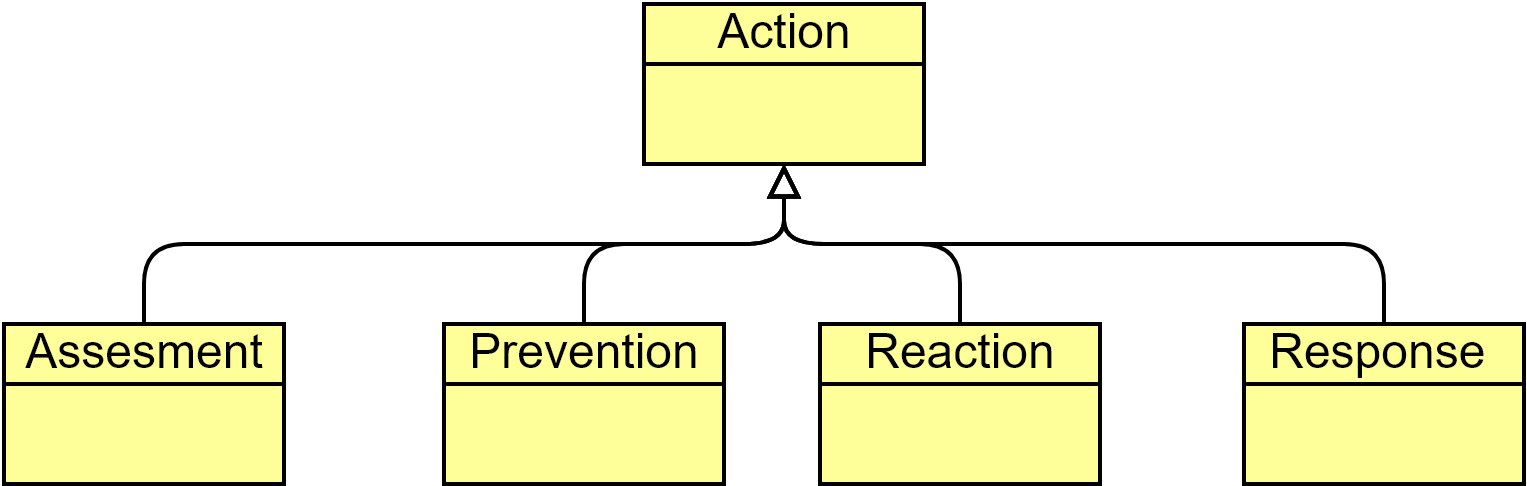
\includegraphics[width=4.36in,height=1.37in]{images/image6.png}
		\caption{Types of actions in a crisis}
		\label{fig:Types_of_actions_in_a_crisis}
	\end{Center}
\end{figure}
%%%%%%%%%%%%%%%%%%%% Figure/Image No: 1 Ends here %%%%%%%%%%%%%%%%%%%%
\end{Center}

``Action''  is a broad term covering all sorts of activities. Under it are depicted four classes of actions: the first two (on the left side of the diagram) are notably occurring before the crisis event happens. The other two (on the right side of the chart) apply to the aftermath. The depiction of the types of actions ordered sequentially along the temporal axis is depicted in Figure \ref{fig:Phases_in_crisis_management} where the crisis event takes a central place. 

\begin{Center}
%%%%%%%%%%%%%%%%%%%% Figure/Image No: 2 starts here %%%%%%%%%%%%%%%%%%%%

\begin{figure}[H]
	\begin{Center}
		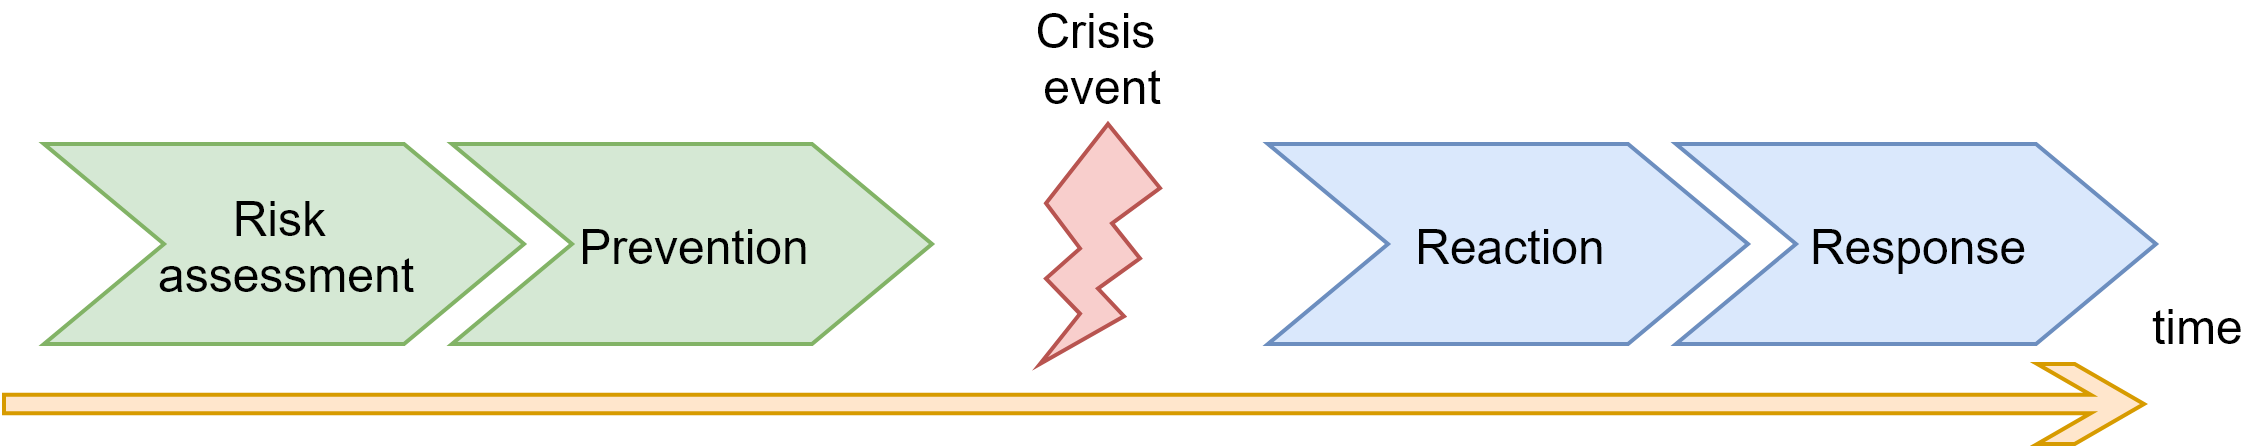
\includegraphics[width=\textwidth]{images/image4.png}
		\caption{Phases in crisis management}
		\label{fig:Phases_in_crisis_management}
	\end{Center}
\end{figure}
%%%%%%%%%%%%%%%%%%%% Figure/Image No: 2 Ends here %%%%%%%%%%%%%%%%%%%%
\end{Center}

The \textit{risk assessment} actions deal with risk identification, estimation of probability for each risk factor to occur. Also, at this stage is investigated the impact from the environmental, economic, social and public health perspectives, including who is impacted, how, and to what degree. 

The \textit{prevention} actions focus on what could be done to mitigate and alleviate the crisis impact in case it occurs. 

The \textit{crisis event} (or period) leads to an unstable and dangerous situation affecting an individual, group, or all of society. 

The \textit{reaction} actions deal with immediate mitigation while the \textit{responses} with medium to long-term mitigate the crisis consequences. These two action types: responses and reactions, which we collectively call \textit{measures}, and in our case \textit{measures to the COVID-19 crisis}, are the primary focus of the dataset. So, next, we define them in this context specifically. 

The \textit{COVID-19 reaction} is what an organisation plans to do to minimise the impact of the pandemics, such as including extra protective equipment for health workers, procurement of additional medical equipment, the introduction of social distancing, more rigorous border controls or their temporary closure. The reactions are actions related to the pandemic poses' health threats: ``a virus makes people sick, and something must be done about that'' . In addition to the pandemic consequences, the reactions have economic and social effects that can be directly observed or indirectly deduced. And so the reaction of the authorities to the virus affects the people too: consider, for example, the social distancing or the lockdown measures. We can say that the reactions are, in fact, to the health threat and that the main topics are anything related to health, pandemics, virus, infection etc. 

The \textit{COVID-19 responses} are measures set in place to compensate for the economic and social consequences of the pandemic crisis and diminish the effects of the authorities' reactions to the threat. Therefore the temporal horizon of the responses is much longer, and the topics they deal with are much broader and challenging to pinpoint. They could be anything related to social, economic, welfare, child care, telework, income support, increase in social protection and many other topics. 

Now, that the dataset domain is set to the COVID-19 reaction and response measures, with a predominant preference for the COVID-19 responses, we describe other criteria and provide some of our assumptions.  

\section{Criteria and assumptions about the data}
\label{sec:criteria}

\begin{itemize}
	\item Identify references to sources of data from discussions with the stakeholders and investigate them. From the selected ones collect text and metadata describing and classifying responses and reactions to the COVID-19 crisis. 
	\item To the extent possible, distinguish between reaction and response measures (as explained in Section \ref{sec:domain-delimitation}) because of the current project scope. 
	\item We assume that the official documents are a reliable source of measure descriptions.
	\item The primary focus is on collecting official texts of various registers (administrative, journalistic, legal, etc.) to enable further exercises to train machine learning models that can identify and distinguish a COVID-19 measure from other texts and, if possible, differences between the reactions and responses.
	\item Selecting the texts with these properties leads to a relatively scarce set of available resources. Therefore no (data) sampling was considered or any tests for the (data) balancing. Mainly we aimed at covering selected initial sources given the apparent degree of (data) representativeness to the semantic domain, which remains to be tested and analysed.
	\item We could identify two text registers (or genres) in the available sources, which is a valuable distinction in the further analysis. First is the journalistic or reportage style of language, which summarises and describes COVID-19 measures. Second is the legal style of language that characterises the source texts from where COVID-19 actions summaries are extracted. Possibly more genres could be identified in a detailed analysis. 
	\item Geographically, we select texts produced in the European Union, both at the EU level, by the institutions and at the member state level, by the national governments. 
	\item We select texts written in English as a first step and as an established limit to the scope, and later, in future work, this can be extended to texts written in the official EU 24 languages.
	\item We consider only texts issued after the beginning of 2020 when the COVID-19 pandemic started.

	\item A basic assumption is that Policy Watch Database (PWDB) is a suitable set of summarised descriptions of what a COVID-19 measure looks like. They cover broader economic and social issues in the area of working and living conditions and intentionally exclude COVID-19 reactions, which focus on public health-related issues. PWDB is a starting point and a pillar in developing this project. 
\end{itemize}

\section{Established data scope: how much is enough?}

Following an investigation and a series of discussions with the project stakeholders, it was decided to set the initial scope to collect data. This scope was set on pragmatic grounds with an awareness of possible extensions in future work.

This section presents the four datasets extracted from another source and constitute the current project dataset, Euro-COVID-19. The detailed description for each dataset is provided in a dedicated section below. Below is an outline of these datasets, along with their subcomponents. Note that the subcomponents are noteworthy at the level of this document to facilitate a deeper understanding of the data, but the dataset distributions merge them into usable wholes. We also provide a codified identifier for each dataset to allow for precise referencing.

\begin{itemize}
	\item \textbf{ds\_pwdb:} Policy Watch Dataset 
        \begin{itemize}
        	\item \textbf{what:} the content published on Eurofound website\footnote{ \href{https://www.eurofound.europa.eu/data/covid-19-eu-policywatch}{COVID-19 EU Policy Watch}}, that is enriched with content crawled from the referenced sources.
        	\item \textbf{why:} because it comprises a collection of manually authored documents summarising the COVID-19 response measures by the member states.
        \end{itemize}
	\item \textbf{ds\_eu\_cellar:} EU Cellar COVID-19 Dataset 
        \begin{itemize}
        	\item \textbf{what:} the EurLex\footnote{ \href{https://eur-lex.europa.eu/homepage.html}{EurLex: the portal to access European Union law} } documents fetched from Cellar\footnote{ \href{https://op.europa.eu/en/publication-detail/-/publication/50ecce27-857e-11e8-ac6a-01aa75ed71a1}{The semantic repository of the Publications Office} } marked with a special ``COVID-19'' tag. And, in addition, Cellar documents about selected EuroVoc\footnote{ \href{https://op.europa.eu/en/web/eu-vocabularies/dataset/-/resource?uri=http://publications.europa.eu/resource/dataset/eurovoc}{EuroVoc: The EU's Multilingual Thesaurus} } concepts (tightly related to COVID-19) dated after the 1st of January 2020.
        	\item \textbf{why:} because Cellar is the official EU semantic repository hosted by the Publications Office containing the official EU. documents. 
        \end{itemize}
	\item \textbf{ds\_eu\_timeline:} EU Action Timeline Dataset 
        \begin{itemize}
        	\item \textbf{what:} documents crawled from the EU action timeline website\footnote{ \href{https://ec.europa.eu/info/live-work-travel-eu/coronavirus-response/timeline-eu-action_en}{Timeline of EU action} }; and documents from the European Commission Press corner\footnote{ \href{https://ec.europa.eu/commission/presscorner/home/en}{Press material from the Commission Spokesperson's Service} } crawled by searching for selected EuroVoc concepts dated after 1st of January 2020.
        	\item \textbf{why:} because it comprises a curated list of official press releases on measures taken by the European Commission (the EU doer).
        \end{itemize}
	\item \textbf{ds\_ireland\_timeline:} Ireland COVID-19 Timeline Dataset
        \begin{itemize}
        	\item \textbf{what:} documents crawled from the Irish Government press corner by searching for pre-selected EuroVoc concepts dated after 1st of January 2020. 
        	\item \textbf{why:} it contains English language texts and constitutes an alternative source of (one) MS measures, which can be used to compare how ds\_pwdb covers a country. 
        \end{itemize}
\end{itemize}

\enlargethispage{1em}

The datasets listed above differ in terms of their internal structure and in terms of the content they cover. Each dataset will be presented in the sections below. A summary of the dataset content classification is provided in  Table \ref{tab:Classification of the dataset content}.

%%%%%%%%%%%%%%%%%%%% Table No: 2 starts here %%%%%%%%%%%%%%%%%%%%
\begin{table}[H]
 			\centering
\begin{tabular}{p{1.25in}p{1.25in}p{1.25in}p{1.25in}}
\hline
%row no:1
\multicolumn{1}{|p{1.25in}}{\Centering \textbf{@en}} & 
\multicolumn{1}{|p{1.25in}}{\Centering \textbf{EU}} & 
\multicolumn{1}{|p{1.25in}}{\Centering \textbf{MS (collectively)}} & 
\multicolumn{1}{|p{1.25in}|}{\Centering \textbf{MS (individual)}} \\
\hhline{----}
%row no:2
\multicolumn{1}{|p{1.25in}}{\Centering Journalistic text} & 
\multicolumn{1}{|p{1.25in}}{\Centering EU actions timeline} & 
\multicolumn{1}{|p{1.25in}}{\Centering Policy Watch DB} & 
\multicolumn{1}{|p{1.25in}|}{\Centering Ireland timeline} \\
\hhline{----}
%row no:3
\multicolumn{1}{|p{1.25in}}{\Centering Legal text} & 
\multicolumn{1}{|p{1.25in}}{\Centering EU Cellar COVID-19} & 
\multicolumn{1}{|p{1.25in}}{\Centering -} & 
\multicolumn{1}{|p{1.25in}|}{\Centering -} \\
\hhline{----}

\end{tabular}\caption{Classification of the dataset content}
\label{tab:Classification of the dataset content}
 \end{table}
\vspace{-1em}
%%%%%%%%%%%%%%%%%%% Table No: 2 ends here %%%%%%%%%%%%%%%%%%%%

In terms of content coverage, we distinguish datasets that cover: the EU measures, the MS measures for all EU states in a single collection, the MS measures segregated for each country. 

In terms of language register\footnote{Register (in Sociolinguistics) is a variety of language used for a particular purpose or in a particular communicative situation. This term is remotely synonym to text type, style and genre.} two major ones are identified that characterise existent texts: (a) \textit{Journalistic or reportage text register} and (b) \textit{formal administrative and legal text register}. The aim here is not to describe these registers but merely identify them as making such a distinction may be of significant relevance in the data analysis phase. 

Datasets pertaining to the journalistic(reportage) text register are

\begin{itemize}
	\item Policy Watch Database 
	\item EU action timeline

	\item Ireland action timeline
\end{itemize}

In the formal administrative and legal text register fall the following datasets

\begin{itemize}
	\item EU Cellar COVID-19 
\end{itemize}

In the next section we proceed with describing the structure for each dataset and some of its peculiarities.

\section{Dataset description: what is inside? }

This section describes the datasets in terms of their structure, scope and manner in which the data have been collected. 

\subsection{Policy watch database (ds\_pwdb)}

Eurofound's COVID-19 EU PolicyWatch (PWDB)\footnote{ PWDB download page  } collates information on the responses of government and social partners to the crisis, as well as gathering examples of company practices aimed at mitigating the social and economic impacts. Data has been mainly provided by the Network of Eurofound Correspondents, with quality control carried out by Eurofound staff.

PWDB includes large-scale government measures and wider collective agreements, as well as regional and local initiatives and support measures for smaller groups of workers. As the situation is evolving, measures are newly implemented, changed or cancelled and replaced at rapid speed. It is planned to update the cases with information on the actual uptake of the main measures. Outside the scope of this database are public health measures, travel and movement restrictions and company-specific job losses. 

The original PWDB contains a rich set of attributes. Only a subset is considered relevant from the business perspective to the current project and is listed in the table below. The original structure is transformed into a simplified form for harmonisation with other datasets and easier usage. The data structure of the transformed core PWDB dataset (ds\_pwdb\_core) is described in Table \ref{tab:dspwdbcore}.

In column BF are provided references to the business features for each data attribute. However, it is not always possible to establish a reliable one to one mapping. Therefore, in some places, we use: the tilde sign ($\sim$) to signify an approximate relation, the plus sign to signify that more than one BF is included or represented by the data attribute.

%%%%%%%%%%%%%%%%%%%% Table No: 3 starts here %%%%%%%%%%%%%%%%%%%%
{
\setlength\extrarowheight{3pt}
\begin{longtable}{p{1.16in}p{3.48in}p{0.62in}}

\endfirsthead
\multicolumn{3}{c}{\textit{continued from previous page}}%\hline
\endhead
\multicolumn{3}{r}{\textit{continued on next page}} \\
\endfoot
\endlastfoot\hline
%row no:1
\multicolumn{1}{|p{1.16in}}{\textbf{Data attribute}} & 
\multicolumn{1}{|p{3.48in}}{\textbf{Description}} & 
\multicolumn{1}{|p{0.62in}|}{\textbf{BF}} \\
\hhline{---}
%row no:2
\multicolumn{1}{|p{1.16in}}{Category} & 
\multicolumn{1}{|p{3.48in}}{Nine\ high-level categories for grouping the COVID-19 measures  (proposed by the EuroFond team\footnote{ About Eurofound }).} & 
\multicolumn{1}{|p{0.62in}|}{BF2} \\
\hhline{---}
%row no:3
\multicolumn{1}{|p{1.16in}}{Subcategory} & 
\multicolumn{1}{|p{3.48in}}{Further categorisation into fine grained categories, under a parent category. The two level taxonomy is not documented here but can be recreated from the dataset. } & 
\multicolumn{1}{|p{0.62in}|}{BF2} \\
\hhline{---}
%row no:4
\multicolumn{1}{|p{1.16in}}{Target group (L1)} & 
\multicolumn{1}{|p{3.48in}}{The database provides target groups for each measure. Target groups are organised on two levels: L1 $\&$  L2. The L1 level broadly differentiates between \textit{workers, businesses} and \textit{citizens}.} & 
\multicolumn{1}{|p{0.62in}|}{BF8} \\
\hhline{---}
%row no:5
\multicolumn{1}{|p{1.16in}}{Target group (L2)} & 
\multicolumn{1}{|p{3.48in}}{The L2 level contains more fine grained distinctions containing 42 specific target groups distinctions in total, including for example: \par \begin{itemize}
	\item Workers: \href{https://static.Eurofound.europa.eu/COVID-19db/targetGroups/self-employed.html}{\textcolor[HTML]{1155CC}{\ul{Self-employed}}}, \href{https://static.Eurofound.europa.eu/COVID-19db/targetGroups/seasonal_workers.html}{\textcolor[HTML]{1155CC}{\ul{Seasonal workers}}}, \href{https://static.Eurofound.europa.eu/COVID-19db/targetGroups/platform_workers.html}{\textcolor[HTML]{1155CC}{\ul{Platform workers}}}, etc. \par 	\item Businesses: \href{https://static.Eurofound.europa.eu/COVID-19db/targetGroups/smes.html}{\textcolor[HTML]{1155CC}{\ul{SMEs}}}, \href{https://static.Eurofound.europa.eu/COVID-19db/targetGroups/start-ups.html}{\textcolor[HTML]{1155CC}{\ul{Start-ups}}}, \href{https://static.Eurofound.europa.eu/COVID-19db/targetGroups/larger_corporations.html}{\textcolor[HTML]{1155CC}{\ul{Larger corporations}}}, etc. \par 	\item Citizens: \href{https://static.Eurofound.europa.eu/COVID-19db/targetGroups/parents.html}{\textcolor[HTML]{1155CC}{\ul{Parents}}}, \href{https://static.Eurofound.europa.eu/COVID-19db/targetGroups/older_citizens.html}{\textcolor[HTML]{1155CC}{\ul{Older citizens}}}, \href{https://static.Eurofound.europa.eu/COVID-19db/targetGroups/migrants.html}{\textcolor[HTML]{1155CC}{\ul{Migrants}}}, etc.
\end{itemize}} & 
\multicolumn{1}{|p{0.62in}|}{BF8} \\
\hhline{---}
%row no:6
\multicolumn{1}{|p{1.16in}}{Country} & 
\multicolumn{1}{|p{3.48in}}{The country where the COVID-19 measure is adopted by the government and social partners.} & 
\multicolumn{1}{|p{0.62in}|}{BF5, BF1} \\
\hhline{---}
%row no:7
\multicolumn{1}{|p{1.16in}}{Involved actors} & 
\multicolumn{1}{|p{3.48in}}{Eurofound identified 757 legislations and other statutory regulations, 452 of which have been created entirely in the context of COVID-19. This section gives an overview of social partner's involvement in designing and implementing these measures.} & 
\multicolumn{1}{|p{0.62in}|}{$ \sim $  (BF1 + BF8)} \\
\hhline{---}
%row no:8
\multicolumn{1}{|p{1.16in}}{Funding} & 
\multicolumn{1}{|p{3.48in}}{The sources of financing the measure, if the measure involves financial expenditures. Some measures do not have fundings. } & 
\multicolumn{1}{|p{0.62in}|}{$ \sim $  BF6} \\
\hhline{---}
%row no:9
\multicolumn{1}{|p{1.16in}}{Type} & 
\multicolumn{1}{|p{3.48in}}{Classification of the document types from where the description of the measures originates. Six types of source documents are distinguished, including legislations, collective agreements, recommendations and company practices.} & 
\multicolumn{1}{|p{0.62in}|}{} \\
\hhline{---}
%row no:10
\multicolumn{1}{|p{1.16in}}{Start $\&$  End dates} & 
\multicolumn{1}{|p{3.48in}}{The time period when the measure is applied.} & 
\multicolumn{1}{|p{0.62in}|}{BF4} \\
\hhline{---}
%row no:11
\multicolumn{1}{|p{1.16in}}{Creation date} & 
\multicolumn{1}{|p{3.48in}}{When the measure entry was created in the database.} & 
\multicolumn{1}{|p{0.62in}|}{$ \sim $  BF3} \\
\hhline{---}
%row no:12
\multicolumn{1}{|p{1.16in}}{Update date} & 
\multicolumn{1}{|p{3.48in}}{When last changes were made to the measure entry description.} & 
\multicolumn{1}{|p{0.62in}|}{$ \sim $  BF3} \\
\hhline{---}
%row no:13
\multicolumn{1}{|p{1.16in}}{Background information} & 
\multicolumn{1}{|p{3.48in}}{A short text providing the context and background information useful to understand the measure description.} & 
\multicolumn{1}{|p{0.62in}|}{BF10} \\
\hhline{---}
%row no:14
\multicolumn{1}{|p{1.16in}}{Content of measure} & 
\multicolumn{1}{|p{3.48in}}{A short text representing the abstract or a concise description of the measure.} & 
\multicolumn{1}{|p{0.62in}|}{BF10} \\
\hhline{---}
%row no:15
\multicolumn{1}{|p{1.16in}}{Content updates} & 
\multicolumn{1}{|p{3.48in}}{Short updates to the content of the measure.} & 
\multicolumn{1}{|p{0.62in}|}{BF10} \\
\hhline{---}
%row no:16
\multicolumn{1}{|p{1.16in}}{Use of measure} & 
\multicolumn{1}{|p{3.48in}}{Information about the results and outcomes of executing/enacting the measure.} & 
\multicolumn{1}{|p{0.62in}|}{BF10} \\
\hhline{---}
%row no:17
\multicolumn{1}{|p{1.16in}}{Title} & 
\multicolumn{1}{|p{3.48in}}{A short text used to identify the measure, place it in context, and convey a minimal summary of its contents.} & 
\multicolumn{1}{|p{0.62in}|}{BF10} \\
\hhline{---}
\caption{The attribute structure for core PWDB dataset (ds\_pwdb\_core)}
\label{tab:dspwdbcore}
\end{longtable}}



%%%%%%%%%%%%%%%%%%%% Table No: 3 ends here %%%%%%%%%%%%%%%%%%%%

In the core dataset, a list of source references is provided. They represent links to the original documents elaborating on the contents of the measure. We proceeded with downloading, cleaning and injecting the content of the sources into the PWD dataset, this way extending it.  
An additional set of data attributes is provided in the extended version of the PWDB dataset, as is listed in  Table \ref{tab:dspwdbext)}.

%%%%%%%%%%%%%%%%%%%% Table No: 4 starts here %%%%%%%%%%%%%%%%%%%%
\begin{table}[H]
 			\centering
\begin{tabular}{p{1.04in}p{4.24in}p{0.39in}}
\hline
%row no:1
\multicolumn{1}{|p{1.04in}}{\textbf{Data attribute}} & 
\multicolumn{1}{|p{4.24in}}{\textbf{Description}} & 
\multicolumn{1}{|p{0.39in}|}{\textbf{BF}} \\
\hhline{---}
%row no:2
\multicolumn{1}{|p{1.04in}}{Source URL} & 
\multicolumn{1}{|p{4.24in}}{The measure descriptions are based on external sources referenced by URLs} & 
\multicolumn{1}{|p{0.39in}|}{} \\
\hhline{---}
%row no:3
\multicolumn{1}{|p{1.04in}}{Source content} & 
\multicolumn{1}{|p{4.24in}}{The content (in simple text) downloaded by accessing the document at the source URL.} & 
\multicolumn{1}{|p{0.39in}|}{BF10} \\
\hhline{---}
%row no:4
\multicolumn{1}{|p{1.04in}}{Source title} & 
\multicolumn{1}{|p{4.24in}}{The title of the source document, if possible to retrieve} & 
\multicolumn{1}{|p{0.39in}|}{BF10} \\
\hhline{---}
%row no:5
\multicolumn{1}{|p{1.04in}}{Source language} & 
\multicolumn{1}{|p{4.24in}}{The language of the source content is determined by a language identification system.} & 
\multicolumn{1}{|p{0.39in}|}{} \\
\hhline{---}

\end{tabular}
\caption{The additional set of attributes constituting the PWBD extension (ds\_pwdb\_ext)}
\label{tab:dspwdbext)}
\end{table}
%%%%%%%%%%%%%%%%%%%% Table No: 4 ends here %%%%%%%%%%%%%%%%%%%%

Finally, the core and the extended dataset variants are merged and provided as a unified PWDB dataset. 

\enlargethispage{1em}

\subsection{EU Cellar COVID-19 dataset (ds\_eu\_cellar)}

The Cellar is the semantic repository of the Publications Office. It stores essential legal documents, general publications and other vital EU level documents. We query this repository to construct the EU level COVID-19 datasets containing the document content and the associated metadata. 

In the context of the current exercise, we distinguish the core and the extended datasets variants, which are results of querying Cellar with two different SPARQL queries.

The core dataset is the result of querying for documents (called works) that are annotated with a special ``COVID-19''  tag in the Cellar repository. The tagging is performed manually by the EurLex team and its contractors. This tag marks documents that have been identified as dealing directly with issues of the COVID-19 pandemic. 

The extended dataset is also the result of querying for documents (called works) in Cellar, which are annotated with any of the pre-selected EuroVoc concepts. We have manually selected concepts from the EuroVoc thesaurus judging whether a concept is or is not relevant to the COVID-19 pandemics. The relevance criteria covers both: the reaction topics, those pertaining to the public health domain, and the response topics, those pertaining to broader social and economic domains (for domain delineation see Section \ref{sec:domain-delimitation} ). The list of selected EuroVoc concepts is provided in  Table \ref{tab:EuroVoc concepts considered highly relevant for COVID-19 document search}. 

%%%%%%%%%%%%%%%%%%%% Table No: 5 starts here %%%%%%%%%%%%%%%%%%%%
{
\setlength\extrarowheight{3pt}
\begin{longtable}{p{2.5in}p{2.96in}}

\endfirsthead
\multicolumn{2}{c}{\textit{continued from previous page}} %\hline
\endhead
\multicolumn{2}{r}{\textit{continued on next page}} \\
\endfoot
\endlastfoot\hline
%row no:1
\multicolumn{1}{|p{2.5in}}{\textbf{Concept URI}} & 
\multicolumn{1}{|p{2.96in}|}{\textbf{Concept preferred label}} \\
\hhline{--}
%row no:2
\multicolumn{1}{|p{2.5in}}{{\fontsize{10pt}{12.0pt}\selectfont http://eurovoc.europa.eu/1005}} & 
\multicolumn{1}{|p{2.96in}|}{{\fontsize{10pt}{12.0pt}\selectfont EU financing}} \\
\hhline{--}
%row no:3
\multicolumn{1}{|p{2.5in}}{{\fontsize{10pt}{12.0pt}\selectfont http://eurovoc.europa.eu/1439}} & 
\multicolumn{1}{|p{2.96in}|}{{\fontsize{10pt}{12.0pt}\selectfont innovation}} \\
\hhline{--}
%row no:4
\multicolumn{1}{|p{2.5in}}{{\fontsize{10pt}{12.0pt}\selectfont http://eurovoc.europa.eu/1633}} & 
\multicolumn{1}{|p{2.96in}|}{{\fontsize{10pt}{12.0pt}\selectfont free movement of persons}} \\
\hhline{--}
%row no:5
\multicolumn{1}{|p{2.5in}}{{\fontsize{10pt}{12.0pt}\selectfont http://eurovoc.europa.eu/1754}} & 
\multicolumn{1}{|p{2.96in}|}{{\fontsize{10pt}{12.0pt}\selectfont illness}} \\
\hhline{--}
%row no:6
\multicolumn{1}{|p{2.5in}}{{\fontsize{10pt}{12.0pt}\selectfont http://eurovoc.europa.eu/1756}} & 
\multicolumn{1}{|p{2.96in}|}{{\fontsize{10pt}{12.0pt}\selectfont respiratory disease}} \\
\hhline{--}
%row no:7
\multicolumn{1}{|p{2.5in}}{{\fontsize{10pt}{12.0pt}\selectfont http://eurovoc.europa.eu/1759}} & 
\multicolumn{1}{|p{2.96in}|}{{\fontsize{10pt}{12.0pt}\selectfont infectious disease}} \\
\hhline{--}
%row no:8
\multicolumn{1}{|p{2.5in}}{{\fontsize{10pt}{12.0pt}\selectfont http://eurovoc.europa.eu/1802}} & 
\multicolumn{1}{|p{2.96in}|}{{\fontsize{10pt}{12.0pt}\selectfont labour market}} \\
\hhline{--}
%row no:9
\multicolumn{1}{|p{2.5in}}{{\fontsize{10pt}{12.0pt}\selectfont http://eurovoc.europa.eu/1854}} & 
\multicolumn{1}{|p{2.96in}|}{{\fontsize{10pt}{12.0pt}\selectfont disease prevention}} \\
\hhline{--}
%row no:10
\multicolumn{1}{|p{2.5in}}{{\fontsize{10pt}{12.0pt}\selectfont http://eurovoc.europa.eu/192}} & 
\multicolumn{1}{|p{2.96in}|}{{\fontsize{10pt}{12.0pt}\selectfont health control}} \\
\hhline{--}
%row no:11
\multicolumn{1}{|p{2.5in}}{{\fontsize{10pt}{12.0pt}\selectfont http://eurovoc.europa.eu/2916}} & 
\multicolumn{1}{|p{2.96in}|}{{\fontsize{10pt}{12.0pt}\selectfont applied research}} \\
\hhline{--}
%row no:12
\multicolumn{1}{|p{2.5in}}{{\fontsize{10pt}{12.0pt}\selectfont http://eurovoc.europa.eu/2923}} & 
\multicolumn{1}{|p{2.96in}|}{{\fontsize{10pt}{12.0pt}\selectfont medical research}} \\
\hhline{--}
%row no:13
\multicolumn{1}{|p{2.5in}}{{\fontsize{10pt}{12.0pt}\selectfont http://eurovoc.europa.eu/3730}} & 
\multicolumn{1}{|p{2.96in}|}{{\fontsize{10pt}{12.0pt}\selectfont health risk}} \\
\hhline{--}
%row no:14
\multicolumn{1}{|p{2.5in}}{{\fontsize{10pt}{12.0pt}\selectfont http://eurovoc.europa.eu/3885}} & 
\multicolumn{1}{|p{2.96in}|}{{\fontsize{10pt}{12.0pt}\selectfont public health}} \\
\hhline{--}
%row no:15
\multicolumn{1}{|p{2.5in}}{{\fontsize{10pt}{12.0pt}\selectfont http://eurovoc.europa.eu/4470}} & 
\multicolumn{1}{|p{2.96in}|}{{\fontsize{10pt}{12.0pt}\selectfont tourism}} \\
\hhline{--}
%row no:16
\multicolumn{1}{|p{2.5in}}{{\fontsize{10pt}{12.0pt}\selectfont http://eurovoc.europa.eu/4505}} & 
\multicolumn{1}{|p{2.96in}|}{{\fontsize{10pt}{12.0pt}\selectfont air transport}} \\
\hhline{--}
%row no:17
\multicolumn{1}{|p{2.5in}}{{\fontsize{10pt}{12.0pt}\selectfont http://eurovoc.europa.eu/5237}} & 
\multicolumn{1}{|p{2.96in}|}{{\fontsize{10pt}{12.0pt}\selectfont research and development}} \\
\hhline{--}
%row no:18
\multicolumn{1}{|p{2.5in}}{{\fontsize{10pt}{12.0pt}\selectfont http://eurovoc.europa.eu/835}} & 
\multicolumn{1}{|p{2.96in}|}{{\fontsize{10pt}{12.0pt}\selectfont aid to undertakings}} \\
\hhline{--}
%row no:19
\multicolumn{1}{|p{2.5in}}{{\fontsize{10pt}{12.0pt}\selectfont http://eurovoc.europa.eu/1280}} & 
\multicolumn{1}{|p{2.96in}|}{{\fontsize{10pt}{12.0pt}\selectfont occupational health}} \\
\hhline{--}
%row no:20
\multicolumn{1}{|p{2.5in}}{{\fontsize{10pt}{12.0pt}\selectfont http://eurovoc.europa.eu/1634}} & 
\multicolumn{1}{|p{2.96in}|}{{\fontsize{10pt}{12.0pt}\selectfont free movement of workers}} \\
\hhline{--}
%row no:21
\multicolumn{1}{|p{2.5in}}{{\fontsize{10pt}{12.0pt}\selectfont http://eurovoc.europa.eu/2062}} & 
\multicolumn{1}{|p{2.96in}|}{{\fontsize{10pt}{12.0pt}\selectfont standard of living}} \\
\hhline{--}
%row no:22
\multicolumn{1}{|p{2.5in}}{{\fontsize{10pt}{12.0pt}\selectfont http://eurovoc.europa.eu/2479}} & 
\multicolumn{1}{|p{2.96in}|}{{\fontsize{10pt}{12.0pt}\selectfont health policy}} \\
\hhline{--}
%row no:23
\multicolumn{1}{|p{2.5in}}{{\fontsize{10pt}{12.0pt}\selectfont http://eurovoc.europa.eu/5891}} & 
\multicolumn{1}{|p{2.96in}|}{{\fontsize{10pt}{12.0pt}\selectfont public awareness campaign}} \\
\hhline{--}
%row no:24
\multicolumn{1}{|p{2.5in}}{{\fontsize{10pt}{12.0pt}\selectfont http://eurovoc.europa.eu/82}} & 
\multicolumn{1}{|p{2.96in}|}{{\fontsize{10pt}{12.0pt}\selectfont working conditions}} \\
\hhline{--}
%row no:25
\multicolumn{1}{|p{2.5in}}{{\fontsize{10pt}{12.0pt}\selectfont http://eurovoc.europa.eu/2473}} & 
\multicolumn{1}{|p{2.96in}|}{{\fontsize{10pt}{12.0pt}\selectfont communications policy}} \\
\hhline{--}
%row no:26
\multicolumn{1}{|p{2.5in}}{{\fontsize{10pt}{12.0pt}\selectfont http://eurovoc.europa.eu/3086}} & 
\multicolumn{1}{|p{2.96in}|}{{\fontsize{10pt}{12.0pt}\selectfont economic consequence}} \\
\hhline{--}
%row no:27
\multicolumn{1}{|p{2.5in}}{{\fontsize{10pt}{12.0pt}\selectfont http://eurovoc.europa.eu/4636}} & 
\multicolumn{1}{|p{2.96in}|}{{\fontsize{10pt}{12.0pt}\selectfont vaccination}} \\
\hhline{--}
%row no:28
\multicolumn{1}{|p{2.5in}}{{\fontsize{10pt}{12.0pt}\selectfont http://eurovoc.europa.eu/5992}} & 
\multicolumn{1}{|p{2.96in}|}{{\fontsize{10pt}{12.0pt}\selectfont economic activity}} \\
\hhline{--}
%row no:29
\multicolumn{1}{|p{2.5in}}{{\fontsize{10pt}{12.0pt}\selectfont http://eurovoc.europa.eu/712}} & 
\multicolumn{1}{|p{2.96in}|}{{\fontsize{10pt}{12.0pt}\selectfont economic support}} \\
\hhline{--}
%row no:30
\multicolumn{1}{|p{2.5in}}{{\fontsize{10pt}{12.0pt}\selectfont http://eurovoc.europa.eu/826}} & 
\multicolumn{1}{|p{2.96in}|}{{\fontsize{10pt}{12.0pt}\selectfont aid to disadvantaged groups}} \\
\hhline{--}
%row no:31
\multicolumn{1}{|p{2.5in}}{{\fontsize{10pt}{12.0pt}\selectfont http://eurovoc.europa.eu/1596}} & 
\multicolumn{1}{|p{2.96in}|}{{\fontsize{10pt}{12.0pt}\selectfont health legislation}} \\
\hhline{--}
%row no:32
\multicolumn{1}{|p{2.5in}}{{\fontsize{10pt}{12.0pt}\selectfont http://eurovoc.europa.eu/2870}} & 
\multicolumn{1}{|p{2.96in}|}{{\fontsize{10pt}{12.0pt}\selectfont quality of life}} \\
\hhline{--}
%row no:33
\multicolumn{1}{|p{2.5in}}{{\fontsize{10pt}{12.0pt}\selectfont http://eurovoc.europa.eu/3956}} & 
\multicolumn{1}{|p{2.96in}|}{{\fontsize{10pt}{12.0pt}\selectfont social sciences}} \\
\hhline{--}
%row no:34
\multicolumn{1}{|p{2.5in}}{{\fontsize{10pt}{12.0pt}\selectfont http://eurovoc.europa.eu/899}} & 
\multicolumn{1}{|p{2.96in}|}{{\fontsize{10pt}{12.0pt}\selectfont economic aid}} \\
\hhline{--}
%row no:35
\multicolumn{1}{|p{2.5in}}{{\fontsize{10pt}{12.0pt}\selectfont http://eurovoc.europa.eu/7983}} & 
\multicolumn{1}{|p{2.96in}|}{{\fontsize{10pt}{12.0pt}\selectfont European Centre for Disease Prevention and Control}} \\
\hhline{--}
%row no:36
\multicolumn{1}{|p{2.5in}}{{\fontsize{10pt}{12.0pt}\selectfont http://eurovoc.europa.eu/83}} & 
\multicolumn{1}{|p{2.96in}|}{{\fontsize{10pt}{12.0pt}\selectfont living conditions}} \\
\hhline{--}
%row no:37
\multicolumn{1}{|p{2.5in}}{{\fontsize{10pt}{12.0pt}\selectfont http://eurovoc.europa.eu/85}} & 
\multicolumn{1}{|p{2.96in}|}{{\fontsize{10pt}{12.0pt}\selectfont social situation}} \\
\hhline{--}
%row no:38
\multicolumn{1}{|p{2.5in}}{{\fontsize{10pt}{12.0pt}\selectfont http://eurovoc.europa.eu/5764}} & 
\multicolumn{1}{|p{2.96in}|}{{\fontsize{10pt}{12.0pt}\selectfont organisation of health care}} \\
\hhline{--}
%row no:39
\multicolumn{1}{|p{2.5in}}{{\fontsize{10pt}{12.0pt}\selectfont http://eurovoc.europa.eu/3552}} & 
\multicolumn{1}{|p{2.96in}|}{{\fontsize{10pt}{12.0pt}\selectfont teleworking}} \\
\hhline{--}
%row no:40
\multicolumn{1}{|p{2.5in}}{{\fontsize{10pt}{12.0pt}\selectfont http://eurovoc.europa.eu/1742}} & 
\multicolumn{1}{|p{2.96in}|}{{\fontsize{10pt}{12.0pt}\selectfont job preservation}} \\
\hhline{--}
%row no:41
\multicolumn{1}{|p{2.5in}}{{\fontsize{10pt}{12.0pt}\selectfont http://eurovoc.europa.eu/886}} & 
\multicolumn{1}{|p{2.96in}|}{{\fontsize{10pt}{12.0pt}\selectfont state of emergency}} \\
\hhline{--}
%row no:42
\multicolumn{1}{|p{2.5in}}{{\fontsize{10pt}{12.0pt}\selectfont http://eurovoc.europa.eu/1926}} & 
\multicolumn{1}{|p{2.96in}|}{{\fontsize{10pt}{12.0pt}\selectfont working environment}} \\
\hhline{--}
%row no:43
\multicolumn{1}{|p{2.5in}}{{\fontsize{10pt}{12.0pt}\selectfont http://eurovoc.europa.eu/4116}} & 
\multicolumn{1}{|p{2.96in}|}{{\fontsize{10pt}{12.0pt}\selectfont health service}} \\
\hhline{--}
%row no:44
\multicolumn{1}{|p{2.5in}}{{\fontsize{10pt}{12.0pt}\selectfont http://eurovoc.europa.eu/5612}} & 
\multicolumn{1}{|p{2.96in}|}{{\fontsize{10pt}{12.0pt}\selectfont protective equipment}} \\
\hhline{--}
%row no:45
\multicolumn{1}{|p{2.5in}}{{\fontsize{10pt}{12.0pt}\selectfont http://eurovoc.europa.eu/837}} & 
\multicolumn{1}{|p{2.96in}|}{{\fontsize{10pt}{12.0pt}\selectfont epidemic}} \\
\hhline{--}
%row no:46
\multicolumn{1}{|p{2.5in}}{{\fontsize{10pt}{12.0pt}\selectfont http://eurovoc.europa.eu/2270}} & 
\multicolumn{1}{|p{2.96in}|}{{\fontsize{10pt}{12.0pt}\selectfont social participation}} \\
\hhline{--}
%row no:47
\multicolumn{1}{|p{2.5in}}{{\fontsize{10pt}{12.0pt}\selectfont http://eurovoc.europa.eu/838}} & 
\multicolumn{1}{|p{2.96in}|}{{\fontsize{10pt}{12.0pt}\selectfont epidemiology}} \\
\hhline{--}
%row no:48
\multicolumn{1}{|p{2.5in}}{{\fontsize{10pt}{12.0pt}\selectfont http://eurovoc.europa.eu/2793}} & 
\multicolumn{1}{|p{2.96in}|}{{\fontsize{10pt}{12.0pt}\selectfont aid programme}} \\
\hhline{--}
%row no:49
\multicolumn{1}{|p{2.5in}}{{\fontsize{10pt}{12.0pt}\selectfont http://eurovoc.europa.eu/3588}} & 
\multicolumn{1}{|p{2.96in}|}{{\fontsize{10pt}{12.0pt}\selectfont restriction of liberty}} \\
\hhline{--}
%row no:50
\multicolumn{1}{|p{2.5in}}{{\fontsize{10pt}{12.0pt}\selectfont http://eurovoc.europa.eu/6781}} & 
\multicolumn{1}{|p{2.96in}|}{{\fontsize{10pt}{12.0pt}\selectfont basic needs}} \\
\hhline{--}
%row no:51
\multicolumn{1}{|p{2.5in}}{{\fontsize{10pt}{12.0pt}\selectfont http://eurovoc.europa.eu/3371}} & 
\multicolumn{1}{|p{2.96in}|}{{\fontsize{10pt}{12.0pt}\selectfont public hygiene}} \\
\hhline{--}
%row no:52
\multicolumn{1}{|p{2.5in}}{{\fontsize{10pt}{12.0pt}\selectfont http://eurovoc.europa.eu/2013}} & 
\multicolumn{1}{|p{2.96in}|}{{\fontsize{10pt}{12.0pt}\selectfont mass media}} \\
\hhline{--}
%row no:53
\multicolumn{1}{|p{2.5in}}{{\fontsize{10pt}{12.0pt}\selectfont http://eurovoc.europa.eu/7131}} & 
\multicolumn{1}{|p{2.96in}|}{{\fontsize{10pt}{12.0pt}\selectfont social impact}} \\
\hhline{--}
%row no:54
\multicolumn{1}{|p{2.5in}}{{\fontsize{10pt}{12.0pt}\selectfont http://eurovoc.europa.eu/3906}} & 
\multicolumn{1}{|p{2.96in}|}{{\fontsize{10pt}{12.0pt}\selectfont freedom of movement}} \\
\hhline{--}
%row no:55
\multicolumn{1}{|p{2.5in}}{{\fontsize{10pt}{12.0pt}\selectfont http://eurovoc.europa.eu/3370}} & 
\multicolumn{1}{|p{2.96in}|}{{\fontsize{10pt}{12.0pt}\selectfont patient rights}} \\
\hhline{--}
%row no:56
\multicolumn{1}{|p{2.5in}}{{\fontsize{10pt}{12.0pt}\selectfont http://eurovoc.europa.eu/4881}} & 
\multicolumn{1}{|p{2.96in}|}{{\fontsize{10pt}{12.0pt}\selectfont social well-being}} \\
\hhline{--}
%row no:57
\multicolumn{1}{|p{2.5in}}{{\fontsize{10pt}{12.0pt}\selectfont http://eurovoc.europa.eu/86}} & 
\multicolumn{1}{|p{2.96in}|}{{\fontsize{10pt}{12.0pt}\selectfont socioeconomic conditions}} \\
\hhline{--}
%row no:58
\multicolumn{1}{|p{2.5in}}{{\fontsize{10pt}{12.0pt}\selectfont http://eurovoc.europa.eu/1758}} & 
\multicolumn{1}{|p{2.96in}|}{{\fontsize{10pt}{12.0pt}\selectfont endemic disease}} \\
\hhline{--}
%row no:59
\multicolumn{1}{|p{2.5in}}{{\fontsize{10pt}{12.0pt}\selectfont http://eurovoc.europa.eu/779}} & 
\multicolumn{1}{|p{2.96in}|}{{\fontsize{10pt}{12.0pt}\selectfont distance learning}} \\
\hhline{--}
%row no:60
\multicolumn{1}{|p{2.5in}}{{\fontsize{10pt}{12.0pt}\selectfont http://eurovoc.europa.eu/6609}} & 
\multicolumn{1}{|p{2.96in}|}{{\fontsize{10pt}{12.0pt}\selectfont self-regulation}} \\
\hhline{--}
%row no:61
\multicolumn{1}{|p{2.5in}}{{\fontsize{10pt}{12.0pt}\selectfont http://eurovoc.europa.eu/6770}} & 
\multicolumn{1}{|p{2.96in}|}{{\fontsize{10pt}{12.0pt}\selectfont disinformation}} \\
\hhline{--}
%row no:62
\multicolumn{1}{|p{2.5in}}{{\fontsize{10pt}{12.0pt}\selectfont http://eurovoc.europa.eu/c\_324b44f1}} & 
\multicolumn{1}{|p{2.96in}|}{{\fontsize{10pt}{12.0pt}\selectfont social media}} \\
\hhline{--}
%row no:63
\multicolumn{1}{|p{2.5in}}{{\fontsize{10pt}{12.0pt}\selectfont http://eurovoc.europa.eu/c\_5b447e3a}} & 
\multicolumn{1}{|p{2.96in}|}{{\fontsize{10pt}{12.0pt}\selectfont crisis management}} \\
\hhline{--}
%row no:64
\multicolumn{1}{|p{2.5in}}{{\fontsize{10pt}{12.0pt}\selectfont http://eurovoc.europa.eu/c\_31da5694}} & 
\multicolumn{1}{|p{2.96in}|}{{\fontsize{10pt}{12.0pt}\selectfont e-Health}} \\
\hhline{--}
%row no:65
\multicolumn{1}{|p{2.5in}}{{\fontsize{10pt}{12.0pt}\selectfont http://eurovoc.europa.eu/c\_60d3928d}} & 
\multicolumn{1}{|p{2.96in}|}{{\fontsize{10pt}{12.0pt}\selectfont patient safety}} \\
\hhline{--}
%row no:66
\multicolumn{1}{|p{2.5in}}{{\fontsize{10pt}{12.0pt}\selectfont http://eurovoc.europa.eu/c\_9b88f778}} & 
\multicolumn{1}{|p{2.96in}|}{{\fontsize{10pt}{12.0pt}\selectfont hospital infection}} \\
\hhline{--}
%row no:67
\multicolumn{1}{|p{2.5in}}{{\fontsize{10pt}{12.0pt}\selectfont http://eurovoc.europa.eu/c\_ece0a719}} & 
\multicolumn{1}{|p{2.96in}|}{{\fontsize{10pt}{12.0pt}\selectfont viral disease}} \\
\hhline{--}
%row no:68
\multicolumn{1}{|p{2.5in}}{{\fontsize{10pt}{12.0pt}\selectfont http://eurovoc.europa.eu/c\_814bb9e4}} & 
\multicolumn{1}{|p{2.96in}|}{{\fontsize{10pt}{12.0pt}\selectfont coronavirus disease}} \\
\hhline{--}
%row no:69
\multicolumn{1}{|p{2.5in}}{{\fontsize{10pt}{12.0pt}\selectfont http://eurovoc.europa.eu/c\_abfaf2ea}} & 
\multicolumn{1}{|p{2.96in}|}{{\fontsize{10pt}{12.0pt}\selectfont disease surveillance}} \\
\hhline{--}
\caption{EuroVoc concepts considered highly relevant for COVID-19 document search}\label{tab:EuroVoc concepts considered highly relevant for COVID-19 document search}
\end{longtable}}
%%%%%%%%%%%%%%%%%%%% Table No: 5 ends here %%%%%%%%%%%%%%%%%%%%

The result of querying Cellar in both cases (core and extended datasets) contains the same data attributes. The difference is in the retrieved documents. The structure of the eu\_cellar dataset is provided in  Table \ref{tab:The attribute structure for eu_cellar dataset}. 

%%%%%%%%%%%%%%%%%%%% Table No: 6 starts here %%%%%%%%%%%%%%%%%%%%
% \begin{table}[h]
%  			\centering
% \begin{tabular}{p{0.99in}p{3.86in}p{0.58in}}
% \hline
{
\setlength\extrarowheight{3pt}
\begin{longtable}{p{1.16in}p{3.48in}p{0.62in}}

\endfirsthead
\multicolumn{3}{c}{\textit{continued from previous page}}%\hline
\endhead
\multicolumn{3}{r}{\textit{continued on next page}} \\
\endfoot
\endlastfoot\hline
%row no:1
\multicolumn{1}{|p{0.99in}}{\textbf{Data attribute}} & 
\multicolumn{1}{|p{3.86in}}{\textbf{Description}} & 
\multicolumn{1}{|p{0.58in}|}{\textbf{BF}} \\
\hhline{---}
%row no:2
\multicolumn{1}{|p{0.99in}}{Work URI} & 
\multicolumn{1}{|p{3.86in}}{The URI, which is uniquely identifying the work.} & 
\multicolumn{1}{|p{0.58in}|}{} \\
\hhline{---}
%row no:3
\multicolumn{1}{|p{0.99in}}{CDM type} & 
\multicolumn{1}{|p{3.86in}}{The\ work type according to the Common Data Model ontology.  } & 
\multicolumn{1}{|p{0.58in}|}{} \\
\hhline{---}
%row no:4
\multicolumn{1}{|p{0.99in}}{Resource type} & 
\multicolumn{1}{|p{3.86in}}{The work type according to the OP classification used in the European inter-institutional exchange of legal documents. The resource types are organised in a classification scheme called Resource Type\footnote{ Resource Type authority table }. } & 
\multicolumn{1}{|p{0.58in}|}{} \\
\hhline{---}
%row no:5
\multicolumn{1}{|p{0.99in}}{EuroVoc concept} & 
\multicolumn{1}{|p{3.86in}}{The EuroVoc concept\footnote{ The EuroVoc thesaurus is represented as Concepts organised in ConceptSchemes following the Simple Knowledge Organisation System (SKOS). } used as a topic and classifier of the document content. The EuroVoc thesaurus is developed by the OP and used in the inter-institutional context. The concepts are organised as taxonomies from the broad to more narrow concepts. } & 
\multicolumn{1}{|p{0.58in}|}{BF2} \\
\hhline{---}
%row no:6
\multicolumn{1}{|p{0.99in}}{Subject matter} & 
\multicolumn{1}{|p{3.86in}}{The subject matter concept used as topic and classifier of the document content. The Subject Matter controlled vocabulary\footnote{ Subject Matter authority table } is developed by the OP and used in the inter-institutional context. The concepts are organised in a classification scheme called subject-matter, or FD\_070\footnote{ FD 070 ATTO table }. } & 
\multicolumn{1}{|p{0.58in}|}{BF2} \\
\hhline{---}
%row no:7
\multicolumn{1}{|p{0.99in}}{Directory code} & 
\multicolumn{1}{|p{3.86in}}{The directory code concept used to organise the legal documents in the EurLEx website. The concepts are organised in a classification scheme called FD\_555\footnote{ FD 555 ATTO table }.} & 
\multicolumn{1}{|p{0.58in}|}{$ \sim $  BF2} \\
\hhline{---}
%row no:8
\multicolumn{1}{|p{0.99in}}{Author} & 
\multicolumn{1}{|p{3.86in}}{The authors of the legal document. The identifier of the authors provided here is from the controlled list called Corporate Body\footnote{ Corporate body authority table }.} & 
\multicolumn{1}{|p{0.58in}|}{BF1} \\
\hhline{---}
%row no:9
\multicolumn{1}{|p{0.99in}}{Date document} & 
\multicolumn{1}{|p{3.86in}}{The date document was issued, entered into force, signed or other date relevant for the document legality.} & 
\multicolumn{1}{|p{0.58in}|}{BF3} \\
\hhline{---}
%row no:10
\multicolumn{1}{|p{0.99in}}{Content} & 
\multicolumn{1}{|p{3.86in}}{The actual content of the legal document, reduced to simple unstructured text.} & 
\multicolumn{1}{|p{0.58in}|}{BF10} \\
\hhline{---}
%row no:11
\multicolumn{1}{|p{0.99in}}{Title} & 
\multicolumn{1}{|p{3.86in}}{The document tile.} & 
\multicolumn{1}{|p{0.58in}|}{BF10} \\
\hhline{---}

% \end{tabular}
\caption{The attribute structure for eu\_cellar dataset}
\label{tab:The attribute structure for eu_cellar dataset}
%  \end{table}
\end{longtable}}
%%%%%%%%%%%%%%%%%%%% Table No: 6 ends here %%%%%%%%%%%%%%%%%%%%

Finally, the core and the extended dataset variants are merged and provided as a unified EU Cellar COVID-19 dataset. 

\subsection{EU action timeline dataset (ds\_eu\_timeline)}

The European Commission (EC) is coordinating a common European response to the coronavirus outbreak. EC is taking resolute action to reinforce our public health sectors and mitigate the socio-economic impact in the European Union. EC is mobilising means to help the Member States coordinate their national responses and provide objective information about the spread of the virus and practical efforts to contain it. 

The timeline of EU actions\footnote{ EU actions timeline website } during the COVID-19 pandemics is a website published by the EC with the most important COVID-19 responses. From 1104 actions (counted on 19/04/2021) published in the press corner only 171 were mentioned on the EU action timeline. So the timeline constitutes a refinement of the noteworthy and an aggregation of the EU actions. 

We crawl this website, and its content is automatically organised using the attributes listed in  Table \ref{tab:dseutimeline}. Unfortunately, only a very limited set of metadata can be identified in the crawled content: title, abstract, date of publication, and the actual content. And we know that the more metadata about a document, the better it is to answer some of the questions mentioned in the project goals section.

Following a discussion with the representatives of Directorate-General for Communication (DG COMM)\footnote{ The Directorate-General for Communication is the Commission department responsible for explaining EU policies to outside audiences. }, we identified a way to recover the possible topics using the name(s) of the authors for each article. This is possible because each author (spokesperson or press officer) is responsible for one or a few topics. These topics are assigned to each press contact who is on the spokesperson's service page\footnote{ Press contacts – Spokesperson's Service - list of possible article authors each covering one or few topics.}. 

What we did was to first extract and structure the information about each person and the topics he/she covers. Then we extended the original crawler to take into consideration this mapping between the person name and the topics. A new data attribute is created for each article containing the array of possible topics that characterise the article. 

Note that the list shall not be read as conjunction, that is: the article is about all of the topics provided; but as a disjunction, which means: the article is about one of the provided topics. 

%%%%%%%%%%%%%%%%%%%% Table No: 7 starts here %%%%%%%%%%%%%%%%%%%%
% \begin{table}[h]
%  			\centering
% \begin{tabular}{p{0.96in}p{3.87in}p{0.5in}}
% \hline
{
\setlength\extrarowheight{3pt}
\begin{longtable}{p{1.16in}p{3.48in}p{0.62in}}

\endfirsthead
\multicolumn{3}{c}{\textit{continued from previous page}}%\hline
\endhead
\multicolumn{3}{r}{\textit{continued on next page}} \\
\endfoot
\endlastfoot\hline

%row no:1
\multicolumn{1}{|p{0.96in}}{\textbf{Data attribute}} & 
\multicolumn{1}{|p{3.87in}}{\textbf{Description}} & 
\multicolumn{1}{|p{0.5in}|}{\textbf{BF}} \\
\hhline{---}
%row no:2
\multicolumn{1}{|p{0.96in}}{Abstract} & 
\multicolumn{1}{|p{3.87in}}{A short summary of the article, an abstract.} & 
\multicolumn{1}{|p{0.5in}|}{$ \sim $  BF3} \\
\hhline{---}
%row no:3
\multicolumn{1}{|p{0.96in}}{Content} & 
\multicolumn{1}{|p{3.87in}}{An extended description of the action as a press release article. } & 
\multicolumn{1}{|p{0.5in}|}{BF10} \\
\hhline{---}
%row no:4
\multicolumn{1}{|p{0.96in}}{Date} & 
\multicolumn{1}{|p{3.87in}}{The date when the press release was published} & 
\multicolumn{1}{|p{0.5in}|}{BF10} \\
\hhline{---}
%row no:5
\multicolumn{1}{|p{0.96in}}{Title} & 
\multicolumn{1}{|p{3.87in}}{The title of the press release article. } & 
\multicolumn{1}{|p{0.5in}|}{$ \sim $  BF10} \\
\hhline{---}
%row no:6
\multicolumn{1}{|p{0.96in}}{Topic} & 
\multicolumn{1}{|p{3.87in}}{A list of possible topics that the article may be about, derived from the author's thematic responsibility.} & 
\multicolumn{1}{|p{0.5in}|}{BF2} \\
\hhline{---}

% \end{tabular}
\caption{The attribute structure for ds\_eu\_timeline}
\label{tab:dseutimeline}

%  \end{table}
\end{longtable}}
%%%%%%%%%%%%%%%%%%%% Table No: 7 ends here %%%%%%%%%%%%%%%%%%%%

\subsection{Ireland COVID-19 timeline dataset}

Ireland was selected as a tryout member state country for which a COVID-19 timeline shall be created similar to the EU action timeline. It was selected because it is the only member state country (UK having just left the EU) that publishes official documents and press releases in English. 

An investigation was conducted searching for a comparable timeline summary of Ireland actions on COVID-19, and none was found. However, the official government website press corner, \href{http://www.gov.ie}{\textcolor[HTML]{1155CC}{\ul{www.gov.ie}}}, was identified as a good source of information. 

``gov.ie''  website is a central portal for government services and information. It combines the websites of Irish government departments and is a trusted source that makes interactions with the government more user-focused.

We decided to use the search service of this website and search for the same set of EuroVoc concepts that were used to retrieve COVID-19 relevant documents from Cellar. The search results are crawled and structured in a dataset using the set of data attributes listed in  Table \ref{tab:dsirelandtimeline}. 

The preferred label of each EuroVoc concept is used as a search term. For each EuroVoc concept, a new search is launched, and only articles that are more recent than the 1st of January 2020 are considered.

%%%%%%%%%%%%%%%%%%%% Table No: 8 starts here %%%%%%%%%%%%%%%%%%%%
% \begin{table}[h]
%  			\centering
% \begin{tabular}{p{1.21in}p{4.06in}p{0.35in}}
% \hline
{
\setlength\extrarowheight{3pt}
\begin{longtable}{p{1.16in}p{3.48in}p{0.62in}}

\endfirsthead
\multicolumn{3}{c}{\textit{continued from previous page}}%\hline
\endhead
\multicolumn{3}{r}{\textit{continued on next page}} \\
\endfoot
\endlastfoot\hline
%row no:1
\multicolumn{1}{|p{1.21in}}{\textbf{Data attribute}} & 
\multicolumn{1}{|p{4.06in}}{\textbf{Description}} & 
\multicolumn{1}{|p{0.35in}|}{\textbf{BF}} \\
\hhline{---}
%row no:2
\multicolumn{1}{|p{1.21in}}{Title} & 
\multicolumn{1}{|p{4.06in}}{The title of the press release article.} & 
\multicolumn{1}{|p{0.35in}|}{BF10} \\
\hhline{---}
%row no:3
\multicolumn{1}{|p{1.21in}}{Content} & 
\multicolumn{1}{|p{4.06in}}{The press release article in simple, clean unstructured text. } & 
\multicolumn{1}{|p{0.35in}|}{BF10} \\
\hhline{---}
%row no:4
\multicolumn{1}{|p{1.21in}}{Published date} & 
\multicolumn{1}{|p{4.06in}}{The date when the press release was published} & 
\multicolumn{1}{|p{0.35in}|}{BF3} \\
\hhline{---}
%row no:5
\multicolumn{1}{|p{1.21in}}{Update date} & 
\multicolumn{1}{|p{4.06in}}{The date when the article was updated.} & 
\multicolumn{1}{|p{0.35in}|}{$ \sim $ BF3} \\
\hhline{---}
%row no:6
\multicolumn{1}{|p{1.21in}}{Content links} & 
\multicolumn{1}{|p{4.06in}}{A list of links available in the text.} & 
\multicolumn{1}{|p{0.35in}|}{} \\
\hhline{---}
%row no:7
\multicolumn{1}{|p{1.21in}}{Campaigns links} & 
\multicolumn{1}{|p{4.06in}}{A list of links to the organised Campaigns} & 
\multicolumn{1}{|p{0.35in}|}{} \\
\hhline{---}
%row no:8
\multicolumn{1}{|p{1.21in}}{Department} & 
\multicolumn{1}{|p{4.06in}}{The government department that was authoring the article. } & 
\multicolumn{1}{|p{0.35in}|}{$ \sim $ BF1} \\
\hhline{---}
%row no:9
\multicolumn{1}{|p{1.21in}}{Policies links} & 
\multicolumn{1}{|p{4.06in}}{The list of links to the broad policy category under which the article is placed.} & 
\multicolumn{1}{|p{0.35in}|}{$ \sim $ BF2} \\
\hhline{---}
%row no:10
\multicolumn{1}{|p{1.21in}}{Keywords} & 
\multicolumn{1}{|p{4.06in}}{A list of keywords assigned by the article authors. } & 
\multicolumn{1}{|p{0.35in}|}{$ \sim $ BF2} \\
\hhline{---}
%row no:11
\multicolumn{1}{|p{1.21in}}{Page type} & 
\multicolumn{1}{|p{4.06in}}{The\ type of article is similar to the classification from the Resource Type authority table used for the ds\_eu\_cellar dataset. The possible types are the following: press release, speech, news, policy information,  reports, etc. } & 
\multicolumn{1}{|p{0.35in}|}{} \\
\hhline{---}

% \end{tabular}

\caption{The attribute structure for ds\_ireland\_timeline}
\label{tab:dsirelandtimeline}
% \end{table}

\end{longtable}}
%%%%%%%%%%%%%%%%%%%% Table No: 8 ends here %%%%%%%%%%%%%%%%%%%%

\section{Architectural overview}

This section presents the technology stack we employ and the design of the workflows for creating the datasets. An overview is depicted in the Figure \ref{fig:Technology_stack_overview} diagram.


%%%%%%%%%%%%%%%%%%%% Figure/Image No: 3 starts here %%%%%%%%%%%%%%%%%%%%
\begin{figure}[h]
	\begin{Center}
		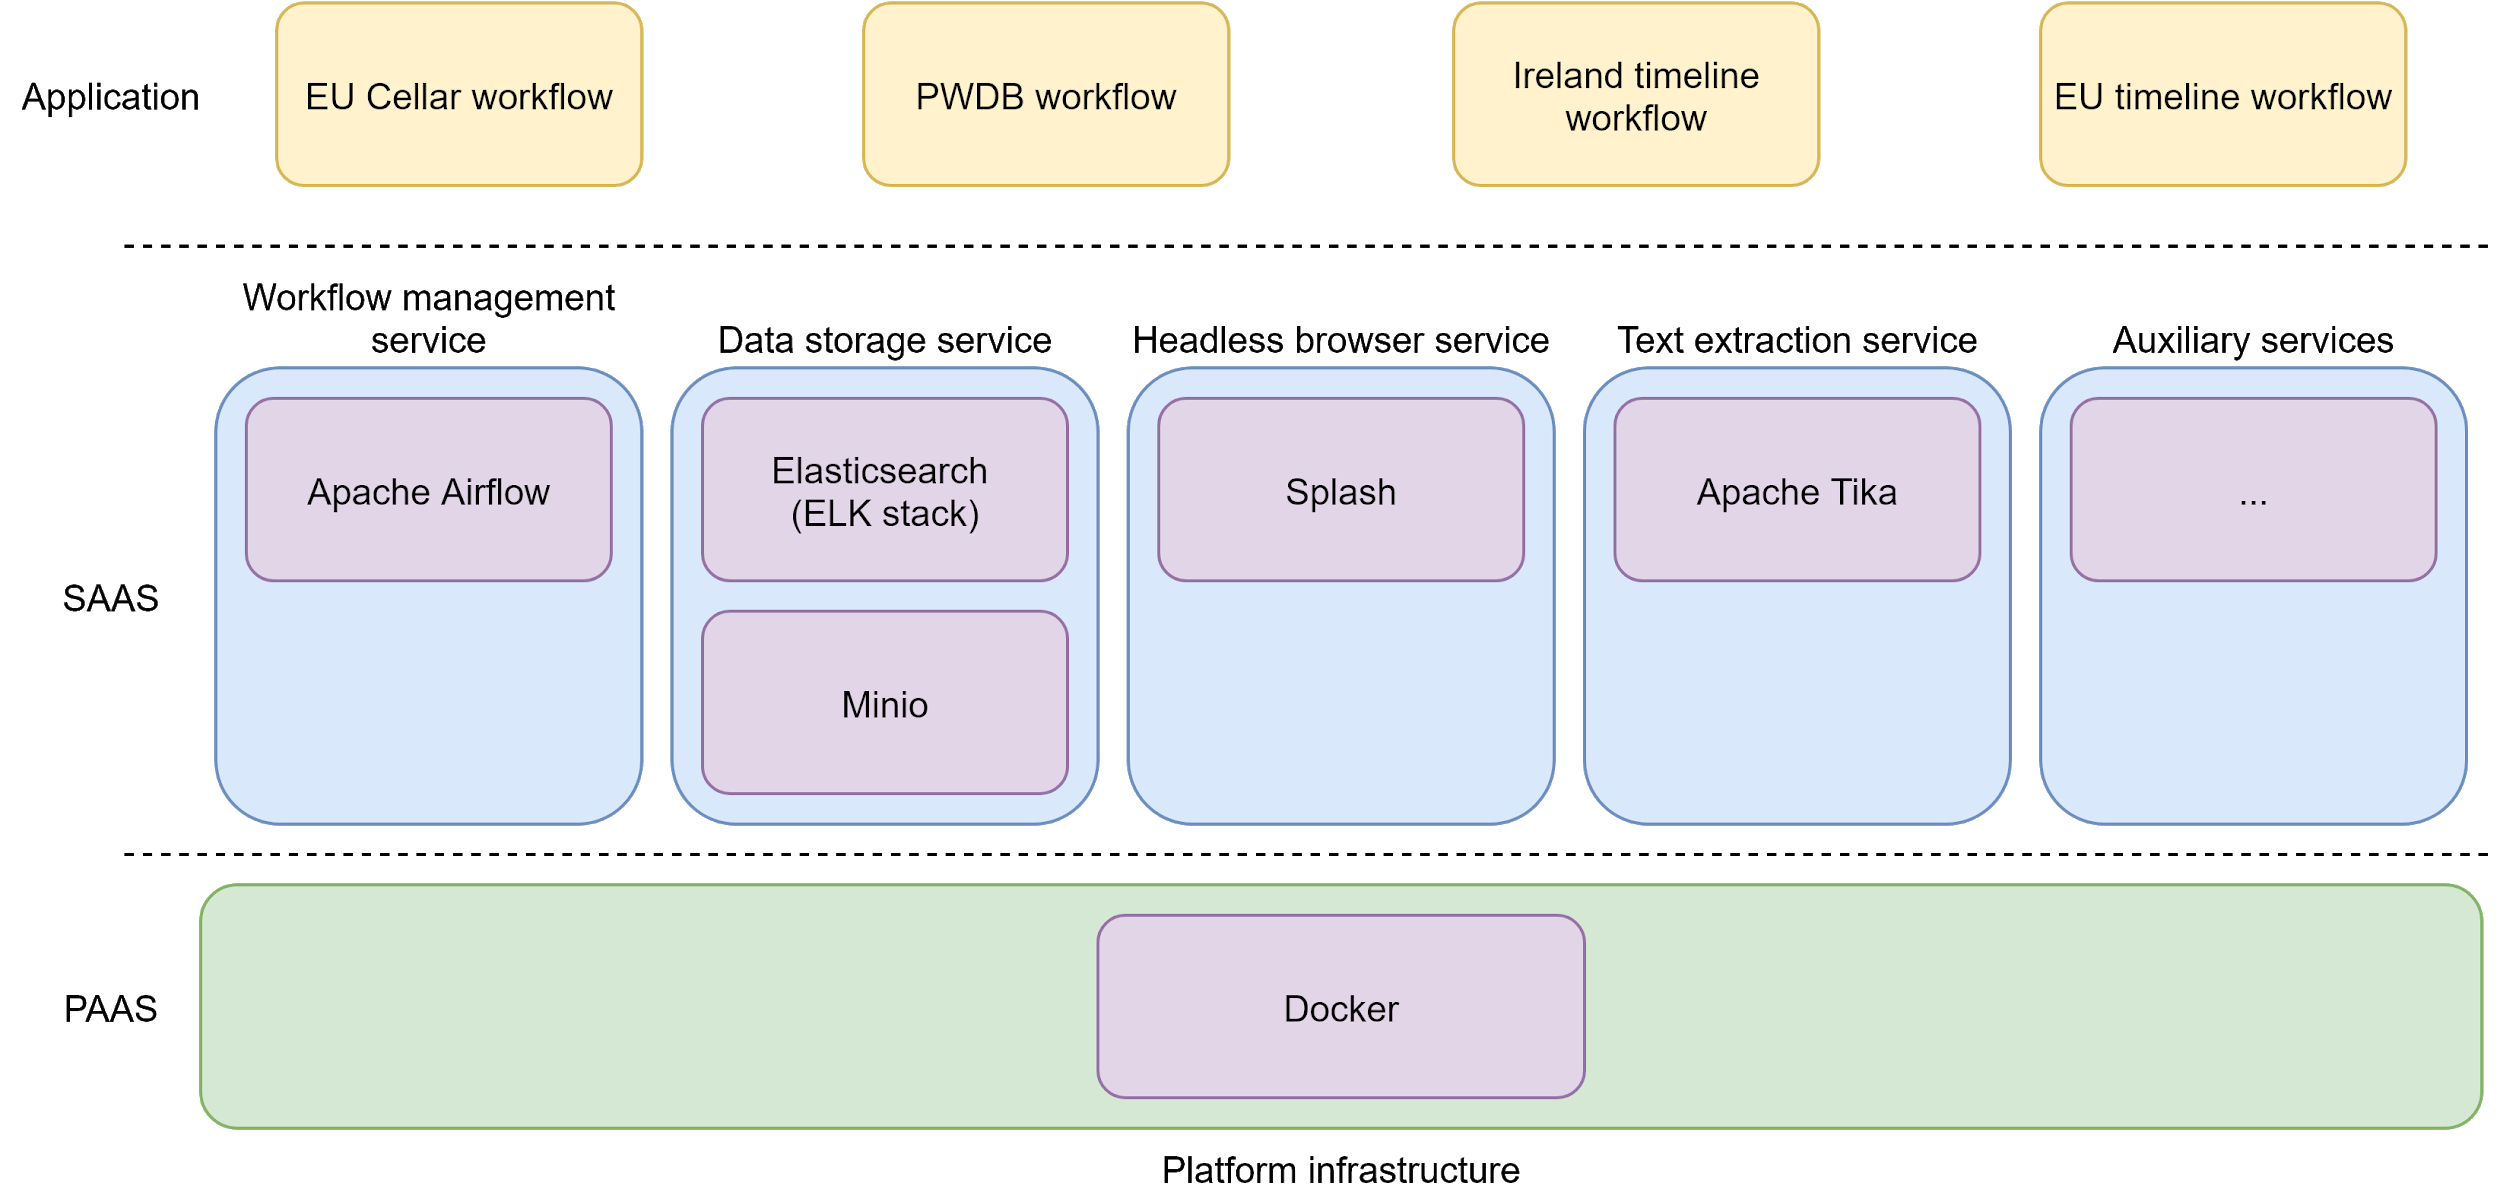
\includegraphics[width=\textwidth]{images/image3.png}
		\caption{Technology stack overview}
		\label{fig:Technology_stack_overview}
	\end{Center}
\end{figure}
%%%%%%%%%%%%%%%%%%%% Figure/Image No: 3 Ends here %%%%%%%%%%%%%%%%%%%%

The diagram in Figure \ref{fig:Technology_stack_overview} is split into three layers: \textit{Platform as a Service (PaaS) layer, Software as a Service (SaaS) layer, and Application layer}. 

\enlargethispage{2em}

At the bottom of the diagram is depicted the infrastructure layer. We have decided to operate based on a platform infrastructure because it abstracts away from the traditional physical servers and allows a deployment virtually in any environment: physical server, virtual machine, cloud. The chosen PaaS technology is Docker\footnote{Docker is a set of platform as a service (PaaS) products that use OS-level virtualization to deliver software in packages called containers. } for its popularity and relative simplicity over alternatives such as Kubernetes\footnote{Kubernetes is an open-source system for automating deployment, scaling, and management of containerized applications.}. 

In the middle of the diagram are depicted five larger blue round-cornered rectangles five. They represent classes of services we're employing in this project. These services are: \textit{workflow management system, data} \textit{storage service, headless browser service, text processing service, }and auxiliary services. We will explain below how each is used after we address the application layer workflow structure. 

In the top part of the diagram is depicted the application layer which contains four workflows, one for each dataset: \textit{EU Cellar workflow}, \textit{EU timeline workflow}, \textit{PWDB workflow}, and \textit{Ireland timeline workflow}. These workflows have a prototypical extract, transform, toad (ETL) structure\footnote{ In computing, extract, transform, load (ETL) is the general procedure of copying data from one or more sources into a destination system which represents the data differently from the source(s) or in a different context than the source(s). The ETL process became a popular concept in the 1970s and is often used in data warehousing. }. The generic ETL process implemented in our workflows is addressed in the next section.

\section{Workflow structure: how it works? }
\label{sec:how-it-works}

This section addresses the general structure of dataset creation workflow. Because it is a simple sequence of tasks, without any major bifurcations we call them pipelines as well. The prototypical pipeline we implement is depicted in Figure \ref{fig:Generic_ETL_process_for_dataset_creation} and can be conceptualised as a sequence of four steps: 

\begin{itemize}
	\item data\textit{ extraction} from the source and storage in the temporary object storage
	\item data \textit{structure transformation} in the temporary storage
	\item data \textit{content transformation} in the temporary storage

	\item final data\textit{ loading} into the document repository
\end{itemize}

The sources of data we employ in this project are: 

\begin{itemize}
	\item Cellar SPARQL endpoint\footnote{ \href{http://publications.europa.eu/webapi/rdf/sparql}{Cellar SPARQL endpoint} } where the EU legal documents are stored and disseminated. 
	\item Eurofound website\footnote{ \href{https://www.eurofound.europa.eu/data/covid-19-eu-policywatch}{Eurofound PWDB download page} } where the PWDB is published.
	\item EU action timeline page

	\item Ireland government press corner page
\end{itemize}

\begin{Center}
%%%%%%%%%%%%%%%%%%%% Figure/Image No: 4 starts here %%%%%%%%%%%%%%%%%%%%
\begin{figure}[h]
	\begin{Center}
		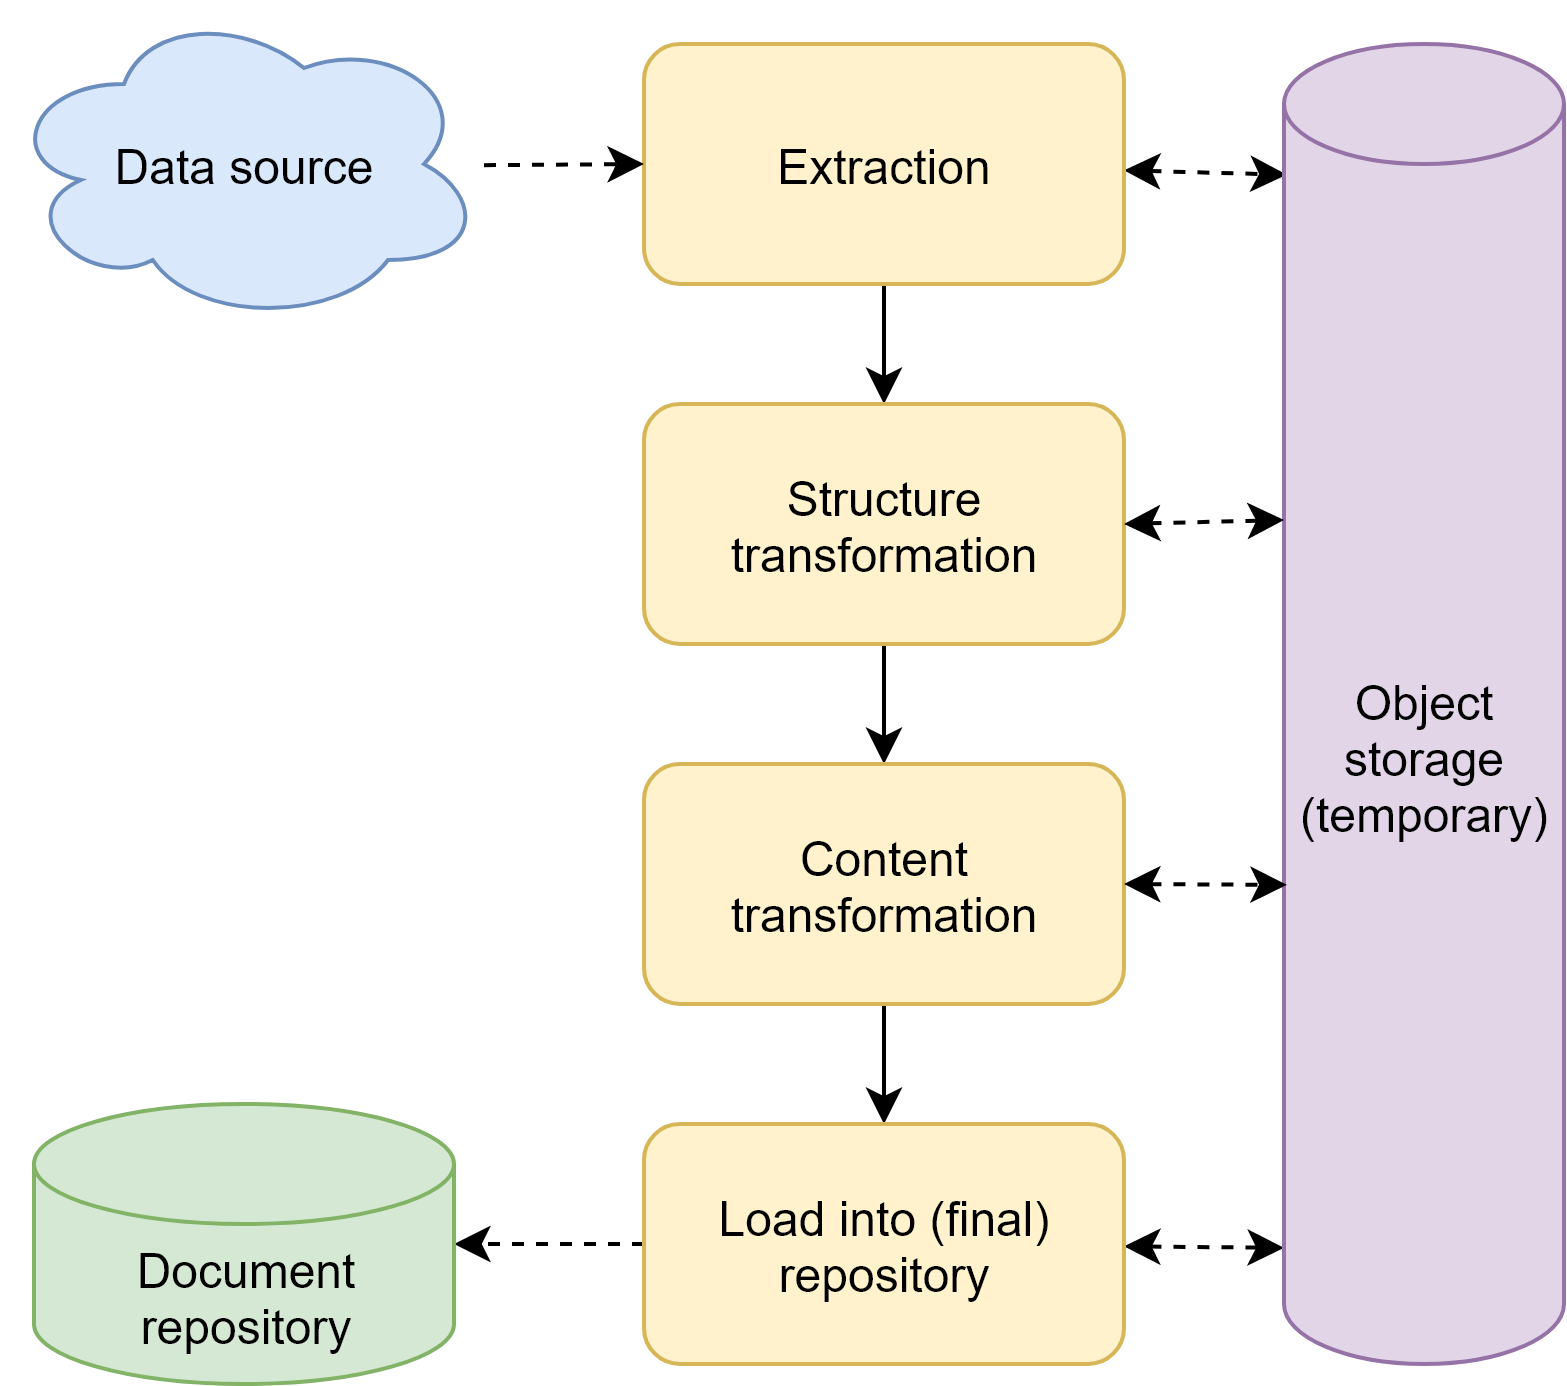
\includegraphics[width=4.24in,height=3.75in]{images/image5.png}
		\caption{Generic ETL process for dataset creation}
		\label{fig:Generic_ETL_process_for_dataset_creation}
	\end{Center}
\end{figure}
%%%%%%%%%%%%%%%%%%%% Figure/Image No: 4 Ends here %%%%%%%%%%%%%%%%%%%%
\end{Center}

\subsection{Extraction}

The process starts with \textit{extracting} the necessary data from the source and storing it in temporary object storage at our premises, making it available for further processing. Doing so enables us to process arbitrarily large amounts of data compared to the alternative of keeping the extracted data in memory, which is relatively limited on the traditional systems. 

Besides simple HTTP requests\footnote{ \href{https://en.wikipedia.org/wiki/Hypertext_Transfer_Protocol}{HTTP} is an application layer protocol for distributed, collaborative, hypermedia information systems. HTTP is the foundation of data communication for the World Wide Web. }, the extraction operations important to mention are the \textit{SPARQL querying} and \textit{Website crawling}. 

SPARQL\footnote{ \href{https://www.w3.org/TR/sparql11-query/}{SPARQL Protocol and RDF Query Language} } is a semantic query language able to retrieve and manipulate data stored in RDF\footnote{ \href{https://www.w3.org/TR/rdf11-concepts/}{Resource Description Framework}  } format. We query Cellar, the European semantic repository, for legal documents annotated with COVID-19 tag or related EuroVoc concepts. 

A \textit{Web crawler\footnote{ \href{https://en.wikipedia.org/wiki/Web_crawler}{Web crawler} }} sometimes called a \textit{spider} and often shortened to \textit{crawler}, is an Internet bot that systematically browses the World Wide Web, typically operated by search engines for the purpose of Web indexing. We developed two crawlers, using Scrapy library\footnote{ \href{https://en.wikipedia.org/wiki/Scrapy}{Scrapy}, a fast high-level web crawling $\&$  scraping framework for Python. }, first to fetch information from the EU action timeline website, and the second one from the Ireland government press corner. Scrapy is a free and open-source web-crawling framework written in Python. Originally designed for web scraping, it can also be used to extract data using APIs or as a general-purpose web crawler.

In the scraping process, often simple HTTP requests are not sufficient for performing full content extraction. Execution of custom JavaScript code is necessary to complete the page loading. For this purpose, headless browser services are typically implemented. They simulate the behaviour of a web browser but without having the interface of one. We employ Splash\footnote{ \href{https://splash.readthedocs.io/en/stable/}{Splash} javascript rendering service } to act as a headless browser. Splash is a javascript rendering service with an HTTP API. It's a lightweight browser with an HTTP API, implemented in Python 3. In combination with Scrapy, Splash allows us to crawl the two web sources successfully. 

One other aspect essential to mention here is that we employ an object storage service called Minio\footnote{ \href{https://min.io/}{MinIO} is an open source implementation of the Amazon S3 storage system.  } for the temporary persistence of the extracted data. MinIO is an Amazon S3 compatible server-side software storage stack. It can handle unstructured data such as photos, videos, log files, backups, and container images with the maximum supported object size of 5TB.

One may argue that such an object storage system is unnecessary as the created datasets, so far, are relatively small in size and can easily fit into the memory of most systems. However, this infrastructure, we intend to extend and use for the processing of much larger datasets exceeding the memory limits. That situation will inevitably invite the usage of such a persistence system, which we foresee and introduce upfront.

\subsection{Structure transformation}

Next, we proceed with \textit{structural transformation} to \textit{normalise} the data representation, simplify it, and increase its usability yet maintaining the maximally helpful structure. For convenience, we aim to represent the data in JSON format following the following system: \textit{an array of objects with a unique identifier and an arbitrary number of atomically typed attributes}. The structure is depicted using an example of prototypical JSON objects in Figure \ref{fig:Example_of_prototypical_JSON_objects_on_the_left_valid_and_on_the_right_an_invalid_structure}. 

The attributes may be of any atomic type, such as numbers, strings, dates, etc. or arrays of atomic types (as depicted on the left side of Figure \ref{fig:Example_of_prototypical_JSON_objects_on_the_left_valid_and_on_the_right_an_invalid_structure}), but not objects or arrays of objects (as depicted on the right side of Figure \ref{fig:Example_of_prototypical_JSON_objects_on_the_left_valid_and_on_the_right_an_invalid_structure}). We discourage, with some exceptions, using the embedded object structures. The reason for it is that the embedded objects are no longer easily accessible in the data frame structures (using the numpy\footnote{ Numpy is a library for the Python programming language, adding support for large, multi-dimensional arrays and matrices, along with a large collection of high-level mathematical functions to operate on these arrays. } or Pandas\footnote{ Pandas is a software library written for the Python programming language for data manipulation and analysis. } libraries). The data frames or other tabular representations are the de facto representation for machine learning and data science exercises, which we plan to undertake in the current project.

\begin{Center}
%%%%%%%%%%%%%%%%%%%% Figure/Image No: 5 starts here %%%%%%%%%%%%%%%%%%%%
\begin{figure}[H]
	\begin{Center}
		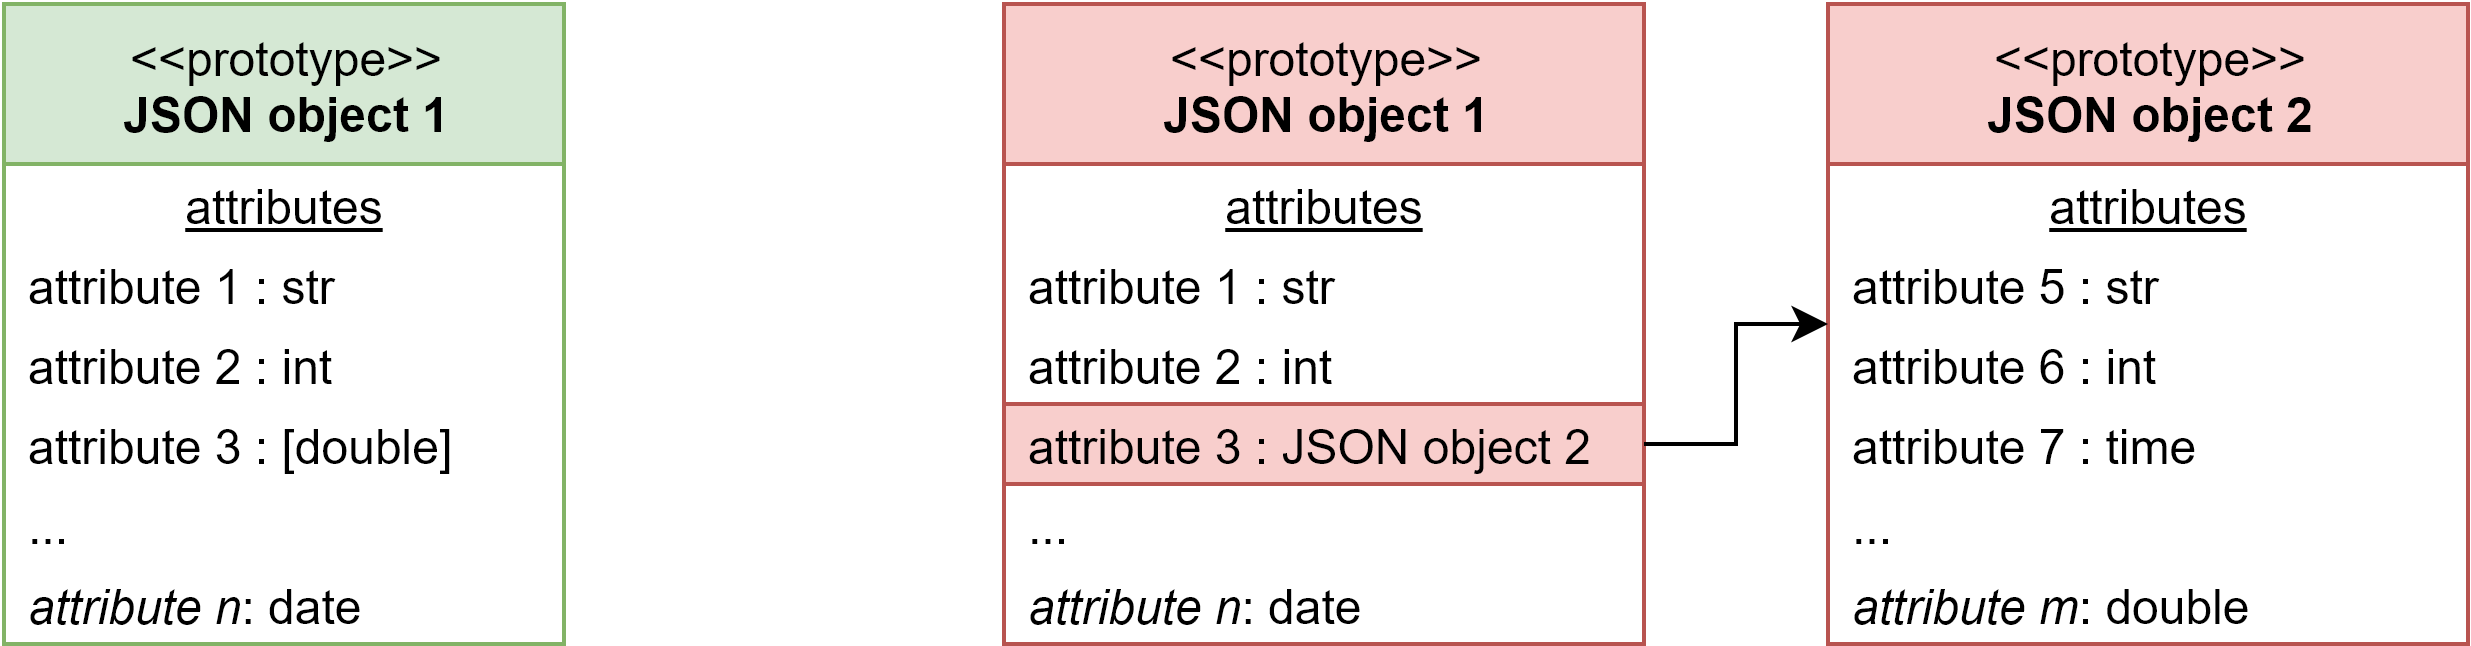
\includegraphics[width=\textwidth]{images/image1.png}
		\caption{Example of prototypical JSON objects, on the left valid and on the right an invalid structure}
		\label{fig:Example_of_prototypical_JSON_objects_on_the_left_valid_and_on_the_right_an_invalid_structure}
	\end{Center}
\end{figure}
%%%%%%%%%%%%%%%%%%%% Figure/Image No: 5 Ends here %%%%%%%%%%%%%%%%%%%%
\end{Center}

For consistency and programming language neutrality, we chose to employ JQ JSON processor\footnote{ ./jq is a lightweight and flexible command-line JSON processor }. The transformation rules are written in JQ language and tailor-made for each data source. As our implementation is entirely written in Python, we use the python library to execute these JQ transformation rules.

\subsection{Content transformation}

fter the data structure is \textit{normalised,} the content transformation generally consists of \textit{text extraction}, \textit{enrichment}, \textit{restructuring, aggregation,} and other operations. 

One peculiarity of this stage is that the initially extracted data contains links and references to other externally available resources. We have carefully analysed and decided to fetch the resources behind selected sets of links. Each dataset includes attributes with such links, which we access and inject the content as an additional attribute. This is what we call content enrichment: injecting extracted content into the dataset. 

The fetched content is in the majority of cases of unpredictable serialisation format, structure and language. Therefore, before it is injected into the dataset, we first \textit{reduce} it to simple texts, which is the foremost valuable data representation for the NLP tasks.

For the \textit{text extraction task,} we decided to use the Apache Tika\footnote{ Apache Tika is a toolkit that detects and extracts metadata and text from over a thousand different file types (such as HTML, PPT, XLS, and PDF). } toolkit. Apache Tika is a library that is used for document type detection and content extraction from various file formats. Internally, Tika uses existing different document parsers and document type detection techniques to detect and extract data. Tika is widely used while developing search engines to index the text contents of digital documents.

Some categorical data attributes are provided as items from a flat fine-grained classification. For practical reasons, it is helpful to reduce the classification scheme. This \textit{restructuring is possible to undergo} by \textit{aggregating} fine-grained categories in terms of more coarse-grained ones. One such example is the target group attribute from PWDB. There are 42 distinct values, which can be roughly categorised as belonging to three more prominent categories. We proceed to inject such aggregations as additional attributes to leverage exploratory data analysis in future stages of the project. 

\subsection{Loading into the repository}

After the structure and content of the data have been restructured, the data is loaded into a repository where it is indexed and made available for querying and full-text search. Because the current datasets are designed for NLP tasks, the full-text search capability is critical. It plays an essential role in the exploratory data analysis and possible data segmentation or partitioning for machine learning experiments. 

For this purpose, we decided to use the Elasticsearch search engine\footnote{ Elasticsearch is a search engine based on the Lucene library. It provides a distributed, multitenant-capable full-text search engine with an HTTP web interface and schema-free JSON documents. } to act as the document repository. It is a real-time distributed and analytic engine that helps in performing various kinds of search mechanisms. It can achieve fast search responses because, instead of searching the text directly, it searches an index instead. Additionally, it supports full-text search, which is completely based on documents instead of tables or schemas that are easier to write queries and manipulate with this textual data. Some of the strongest points of elastic search are:

\begin{itemize}
	\item Performing and combining various kinds of searches irrespective of their data type.
	\item Querying can retrieve data in any form required.
	\item Analyzing billions of records in a few seconds.
	\item Aggregating data enables us to explore trends and patterns.
\end{itemize}

When the datasets are loaded into the Elasticsearch, they are easily explorable using Kibana\footnote{ Kibana is a data visualization dashboard software for Elasticsearch. It provides visualization capabilities on top of the content indexed on an Elasticsearch cluster. } discovery and dashboard functionality. Kibana offers histograms, line graphs, pie charts, sunbursts, geospatial map displays, and other standard visualisation options and the opportunity to create unique visualisations. It also makes it possible for users to spot and analyse relationships or anomalies in the data. Furthermore, the datasets are available for use in machine learning experiments and exploratory data analysis. 

\section{Workflow management system}

The workflows mentioned above are deployed and executed in a workflow management system. Doing so drives automation and leads to increased control, transparency and trust in the execution results. It allows for close monitoring of each step, schedule executions, increased connectivity, eliminates manual tasks, reduces errors, retries on failure, and investigates causes and visualises the workflow, control panel, and other benefits. 

We have chosen Apache Airflow system\footnote{ Apache Airflow is an open-source workflow management platform. It started at Airbnb in October 2014 as a solution to manage the company's increasingly complex workflows. } due to its architectural choices, maturity, rich set of features, strong community, rich set of integrations and plugins, and because a system implemented in Python fits well our Python predominant technical stack. 

Airflow is a platform to programmatically author, schedule and monitor workflows. It is written in Python, and workflows are created via Python scripts, called DAGs (Directed Acyclic Graphs). An example DAG structure is depicted in Figure \ref{fig:Example_of_a_DAG_structure}. 

Airflow is designed under the principle of ``\textit{configuration as code}'' . While other ``\textit{configuration as code}''  workflow platforms exist using markup languages like XML, using Python allows developers to import libraries and classes to help them create their workflows.

\begin{Center}
%%%%%%%%%%%%%%%%%%%% Figure/Image No: 6 starts here %%%%%%%%%%%%%%%%%%%%
\begin{figure}[H]
	\begin{Center}
		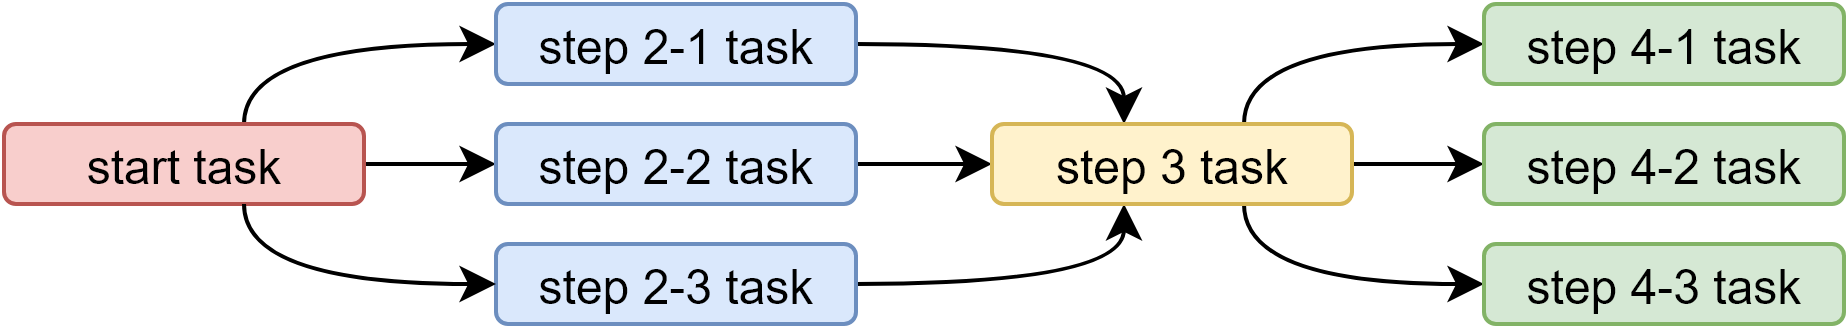
\includegraphics[width=\textwidth]{images/image2.png}
		\caption{Example of a DAG structure}
		\label{fig:Example_of_a_DAG_structure}
	\end{Center}
\end{figure}
%%%%%%%%%%%%%%%%%%%% Figure/Image No: 6 Ends here %%%%%%%%%%%%%%%%%%%%
\end{Center}

Airflow uses directed acyclic graphs (DAGs\footnote{ A DAG is a collection of all the tasks you want to run, organized in a way that reflects their relationships and dependencies. }) to manage workflow orchestration. Tasks and dependencies are defined in Python and then Airflow manages the scheduling and execution. DAGs can be run either on a defined schedule (e.g. hourly or daily) or based on external event triggers.

DAG, or directed acyclic graphs, are a collection of all of the tasks, units of work in the pipeline. The tasks are organised by their relationships and dependencies between each other. A directed acyclic graph implies that your pipeline can only move forwards, not backwards. A task can retry, but a task can't be rerun after it has completed and another task downstream has begun.

Using Airflow enables us to organise our pipelines as DAGs, develop project-specific functionality and incorporate it seamlessly into the workflow architecture to deploy and execute in a robust environment easily.

\section{Limitations and future work}

In the process of developing the current dataset, a number of limitations were set to the scope of this project. This section covers a non-exhaustive list of these limitations and how they may be addressed in future work.

Currently, the dataset is limited to the English language. In future work, the dataset can be expanded to cover member state measures individually. Doing so will inevitably lead to creating a multilingual dataset containing texts in 24 official European languages. This is mainly because the authorities publish the measures in that country's official language(s).

Using different text registers implies a disparate treatment of texts in the analysis and processing pipelines. Developing a mechanism to summarise a document to extract measure description from it, as, for example, would be necessary for large legal texts, would be of tremendous benefit for harmonisation of the dataset content across various sources. Addressing this in future work will yield an advantage for the exploratory data analysis and other machine learning exercises.

Another axis of homogenisation would be to bring all the texts to a common language, such as English, for example. To do so would necessitate translation services, which at the moment were not used. Having done so will decrease the linguistic fragmentation of the dataset, leading to a larger homogeneous corpus, which increases the statistical significance of the results produced based on this dataset.

\enlargethispage{2em}



\section{Introduction}

This document aims at describing how was created the \textit{Euro-COVID-19} dataset comprising texts and metadata on COVID-19 crisis measures taken by the European Union (EU) and the European Member States (MS). The creation of this dataset belongs to the SemCovid project financed by the Open Data Portal unit from the European Publications Office, which is described elsewhere. 

In the Euro-COVID-19 dataset, data are collected from various sources, each providing content with different characteristics and available metadata. What is fetched from a selected source we also call a dataset due to its internal homogeneity and difference to the content available from other sources. Thus we say that the \textit{Euro-COVID-19 dataset} is a composition of different datasets.

Further in the document, we provide some of the underlying assumptions, a summary of methodological considerations, a description of the collected data and the technical stack used to perform the data processing. 

A dataset shall fulfil a clearly defined goal. That is why, before diving into the \textit{hows} of its creation, we first iterate through its whys.

\section{Project goals: the whys}
\label{sec:goals}

The current project goals originate from two stakeholders, whose interests differ in a complementary manner. The EU Open Data Portal team has an investigative novelty-seeking research orientation, while the Eurofound team is pragmatically oriented to satisfy the business needs of the European policymakers. The Eurofound team is in particular interested in the area of working and living conditions for the EU citizens.

From a research perspective, this project sets out to \textit{investigate and establish the semantic mapping of the European Union (EU) and Member States (MS) response (defined in Section \ref{sec:domain-delimitation}) to the COVID-19 crisis in the area of living and working conditions.} This goal can be further elaborated in terms of the following research questions:

\begin{enumerate}
	\item How do the measures compare between Member States collectively and the EU regarding the issues they address, various types of categorisation and degree of content similarity?
	\item How do the measures compare between the Member States individually and also to the EU measures? 
	\item What are the emerging topics in the dataset(s), and how did they evolve over time? 
\end{enumerate}

After discussing the business needs of policymakers with the Eurofound team, a set of prototypical business interests emerged that is best expressed as the following questions:

\begin{enumerate}
	\item Who has done what on which issue? What acting bodies are involved, and which categories of responses are used for classification?
	\item Who pays for the measures and how much? What sources of financing are employed, and what amounts are allocated for each measure or issue?
	\item Who benefits from the measure outcomes? What are the target groups for each measure?
	\item Where is the measure applicable? What is the territorial coverage of the measure? 
	\item When is the measure executed? When is the measure adopted, and how long does it last? 
\end{enumerate}

\section{Business features: the whats}

To answer the above business question, we further ask ourselves what sort of properties or features (BF) shall be available in the datasets to enable answer computation. Having articulated these features explicitly serves as a compass in the data collection and data processing processes. And where the automation has reached its limitation, the same compass will indicate what sort of data shall be collected/produced and published by the data providers in the future. Table \ref{tab:Business features that necessary to answer the business questions} summarises the business features required by the business questions (BQ) listed in Section \ref{sec:goals}.

To give you an example of how the business questions related to the business features, let's take BF8: the target group feature in Table \ref{tab:Business features that necessary to answer the business questions}. The dataset needs to provide explicitly in a dedicated field the information about the target groups of the measure to answer the business question ``Who benefits from the measure outcomes?''  which is relevant to the policymakers. 


%%%%%%%%%%%%%%%%%%%% Table No: 1 starts here %%%%%%%%%%%%%%%%%%%%
% \begin{table}[h]
%  			\centering
% \begin{tabular}{p{0.33in}p{1.64in}p{3.47in}}
% \hline

{
\setlength\extrarowheight{3pt}
\begin{longtable}{p{1.16in}p{3.48in}p{0.62in}}

\endfirsthead
\multicolumn{3}{c}{\textit{continued from previous page}}%\hline
\endhead
\multicolumn{3}{r}{\textit{continued on next page}} \\
\endfoot
\endlastfoot\hline

%row no:1
\multicolumn{1}{|p{0.33in}}{\Centering \textbf{ID}} & 
\multicolumn{1}{|p{1.64in}}{\Centering \textbf{Business feature}} & 
\multicolumn{1}{|p{3.47in}|}{\Centering \textbf{Description}} \\
\hhline{---}
%row no:2
\multicolumn{1}{|p{0.33in}}{BF1} & 
\multicolumn{1}{|p{1.64in}}{adopting entity} & 
\multicolumn{1}{|p{3.47in}|}{The organisation that adopts the COVID measure. } \\
\hhline{---}
%row no:3
\multicolumn{1}{|p{0.33in}}{BF2} & 
\multicolumn{1}{|p{1.64in}}{categories} & 
\multicolumn{1}{|p{3.47in}|}{A classification of the measure following a well-defined scheme manually assigned by the data provider. } \\
\hhline{---}
%row no:4
\multicolumn{1}{|p{0.33in}}{BF3} & 
\multicolumn{1}{|p{1.64in}}{issue date} & 
\multicolumn{1}{|p{3.47in}|}{The date when the measure is published.} \\
\hhline{---}
%row no:5
\multicolumn{1}{|p{0.33in}}{BF4} & 
\multicolumn{1}{|p{1.64in}}{temporal coverage } & 
\multicolumn{1}{|p{3.47in}|}{The beginning and the end dates of the measure applicability or execution leading to a duration definition.} \\
\hhline{---}
%row no:6
\multicolumn{1}{|p{0.33in}}{BF5} & 
\multicolumn{1}{|p{1.64in}}{spatial coverage } & 
\multicolumn{1}{|p{3.47in}|}{The definition of spatial coverage where the measure is applicable. Usually denoted by a codified reference to a territorial unit (country/region). } \\
\hhline{---}
%row no:7
\multicolumn{1}{|p{0.33in}}{BF6} & 
\multicolumn{1}{|p{1.64in}}{sources of financing} & 
\multicolumn{1}{|p{3.47in}|}{The mention of the financing source(s): usually denoted by a reference to an EU programme, special national or international fund, or a generic label such as ``own funds''  or ``national budget'' . } \\
\hhline{---}
%row no:8
\multicolumn{1}{|p{0.33in}}{BF7} & 
\multicolumn{1}{|p{1.64in}}{funding amounts} & 
\multicolumn{1}{|p{3.47in}|}{The total amount of money allocated to or spend for a particular source of financing. } \\
\hhline{---}
%row no:9
\multicolumn{1}{|p{0.33in}}{BF8} & 
\multicolumn{1}{|p{1.64in}}{recipients\ $\&$   beneficiaries (target groups)} & 
\multicolumn{1}{|p{3.47in}|}{The\ groups\ which shall benefit from the measure. Beneficiaries targeted by the action. The beneficiaries may be expressed either as groups of entities (e.g. SMEs, self-employed, etc.),   demographically defined groups (e.g. elderly over 65, single-parent families, etc.) or functionally defined roles (e.g. doctors, policemen etc.).} \\
\hhline{---}
%row no:10
\multicolumn{1}{|p{0.33in}}{BF9} & 
\multicolumn{1}{|p{1.64in}}{semantic similarity} & 
\multicolumn{1}{|p{3.47in}|}{In comparative text analysis studies, the semantic similarity represents how close is the meaning of two texts} \\
\hhline{---}
%row no:11
\multicolumn{1}{|p{0.33in}}{BF10} & 
\multicolumn{1}{|p{1.64in}}{textual description} & 
\multicolumn{1}{|p{3.47in}|}{The textual description of the measure. } \\
\hhline{---}
%row no:12
\multicolumn{1}{|p{0.33in}}{BF11} & 
\multicolumn{1}{|p{1.64in}}{topics} & 
\multicolumn{1}{|p{3.47in}|}{Topics of the measure automatically discovered by the machine learning techniques. } \\
\hhline{---}
% \end{tabular}
\caption{Business features that necessary to answer the business questions}
\label{tab:Business features that necessary to answer the business questions}
%  \end{table}
\end{longtable}
}
%%%%%%%%%%%%%%%%%%%% Table No: 1 ends here %%%%%%%%%%%%%%%%%%%%

Next, in Table \ref{tab:bq2bf} we provide a mapping of business questions (BQs) to business feature (BFs). This mapping represents the information needs that has to be satisfied before a business question can be answered. Consequently in the dataset creation process, we aim at gathering as many BFs as possible. 

\begin{landscape}
% Please add the following required packages to your document preamble:
% \usepackage{booktabs}
% \usepackage{multirow}
% \usepackage{longtable}
% Note: It may be necessary to compile the document several times to get a multi-page table to line up properly
\begin{longtable}[c]{@{}cp{5cm}llllllllllc@{}}
	\toprule
	\multirow{2}{*}{\textbf{Id}} & \multicolumn{1}{c}{\multirow{2}{*}{\textbf{Core Business Question}}} & \multicolumn{11}{c}{\textbf{Business Feature}} \\* \cmidrule(l){3-13} 
	& \multicolumn{1}{c}{} & BF1 & BF2 & BF3 & BF4 & BF5 & BF6 & BF7 & BF8 & BF9 & BF10 & BF11 \\* \cmidrule(r){1-13}
	\endfirsthead
	%
	\multicolumn{13}{c}%
	{{\bfseries Table \thetable\ continued from previous page}} \\
	\toprule
	\multirow{2}{*}{\textbf{Id}} & \multicolumn{1}{c}{\multirow{2}{*}{\textbf{Core Business Question}}} & \multicolumn{11}{c}{\textbf{Business Feature}} \\* \cmidrule(l){3-13} 
	& \multicolumn{1}{c}{} & BF1 & BF2 & BF3 & BF4 & BF5 & BF6 & BF7 & BF8 & BF9 & BF10 & BF11 \\* \cmidrule(r){1-2}
	\endhead
	%
	\bottomrule
	\endfoot
	%
	\endlastfoot
	%
	\textbf{BQ1} & Who has adopted what Covid19 measures and which issues they address? & \multicolumn{1}{c}{x} & \multicolumn{1}{c}{x} &  &  &  &  &  &  &  &  & x \\
	\textbf{BQ2} & When is the measure adopted and how long it shall last? &  &  & \multicolumn{1}{c}{x} & \multicolumn{1}{c}{x} &  &  &  &  &  &  & \multicolumn{1}{l}{} \\
	\textbf{BQ3} & Where is the measure applicable? &  &  &  &  & \multicolumn{1}{c}{x} &  &  &  &  &  & \multicolumn{1}{l}{} \\
	\textbf{BQ4} & What are the themes and topics applicable to measures? &  & \multicolumn{1}{c}{x} &  &  &  &  &  &  &  &  & x \\
	\textbf{BQ5} & Who pays and how much for each measure and where do the money come from? & \multicolumn{1}{c}{x} &  &  &  &  & \multicolumn{1}{c}{x} & \multicolumn{1}{c}{x} &  &  &  & \multicolumn{1}{l}{} \\
	\textbf{BQ6} & Who are the beneficiaries of the measures? What are the target groups of the measure? &  &  &  &  &  &  &  & \multicolumn{1}{c}{x} &  &  & \multicolumn{1}{l}{} \\
	\textbf{BQ7*} & How do the measures compare between Member States collectively and the EU in terms of addressed issues, categories and similarity? &  & \multicolumn{1}{c}{x} &  &  &  &  &  &  & \multicolumn{1}{c}{x} & \multicolumn{1}{c}{x} & x \\
	\textbf{BQ8*} & How do the measures compare between the individual Member States? &  & \multicolumn{1}{c}{x} &  &  &  &  &  &  & \multicolumn{1}{c}{x} & \multicolumn{1}{c}{x} & x \\
	\textbf{BQ9*} & How did the issues / topics evolved over time in Covid19 measures? &  & \multicolumn{1}{c}{x} & \multicolumn{1}{c}{x} &  &  &  &  &  &  & \multicolumn{1}{c}{x} & x \\* \bottomrule
	\caption{Business question (BQ) to business feature (BF) mapping}
	\label{tab:bq2bf}\\
\end{longtable}
\end{landscape}

Based on the above information we can already sketch the structure of a dataset. We aim at collecting texts describing of COVID-19 response measures (the BF10) with associated metadata representing BF1 -- BF8. Later on we will compute the document semantic similarity (BF9) and the topic models (BF11).

\section{Building a dataset: the how}

A dataset is a remarkable thing, not so much because it is a collection of data records, but because of the properties that it acquires if it is well-designed and carefully constructed. The guiding principles for conceiving a good dataset cannot be strictly defined but rely heavily on the good sense and clear thinking of the people involved and \textit{feedback from a consensus of users}. For this, deciding upfront, \textit{``What is the dataset for?''}, \textit{``How will it be used?''} and \textit{``What are the project goals?''} plays a crucial role in its design. Answers to these questions have already been provided in the section above. 

The general approach for building this dataset is as follows. From interactions with the stakeholders it is important to identify the relevant sources of data. The sources are assessed whether they data are structured or unstructured, what business features are available and how the data can be fetched. After the assessment the most relevant sources are chosen, establishing the scope of the dataset, and the extraction and transformation procedures are specified (see Section \ref{sec:how-it-works}). It is important to note that not all BFs are available from each data source, therefore to the extent possible, missing BFs shall be deduced from existent data or explain why that is not possible and accept the limitation of answering only a part of BQs. 

Next we provide a few considerations for building a textual dataset, which are similar to those for building a document corpus. The following sections, Section \ref{sec:domain-delimitation} and Section \ref{sec:criteria} will further address how we delineate the domain and under what criteria and assumptions operate.

In addition, if the dataset involves the organisation of textual content (linguistic data), then it is important to understand and take into consideration \textit{how language in general works}. One needs to pay particular attention to the \textit{communicative functions\footnote{ \href{https://en.wikipedia.org/wiki/Metafunction}{Metafunction} is a systematic cluster, which groups semantic systems that make meanings of a related kind.  }} and the \textit{community} in which the texts arise. However unsteady is the notion of \textit{representativeness\footnote{ \href{https://en.wikipedia.org/wiki/Representativeness_heuristic}{Representativeness heuristic} is simply described as assessing similarity of objects and organizing them based around the category prototype.  }}, it is an unavoidable one in the dataset design, and others such as \textit{sample} and \textit{balance} need to be faced as well. Therefore the \textit{linguistic dataset} builders should strive to make the dataset as representative as possible of the language and purpose for which it is chosen. 

Any selection must be made on some criteria and the first major step in linguistic dataset building is the determination of the criteria on which the sources and the text that form the dataset will be selected.

\begin{enumerate}
	\item The \textit{text register\footnote{ \href{https://en.wikipedia.org/wiki/Register_(sociolinguistics)}{Text register} }}, that is a variety of language used for a particular purpose or in a particular communicative situation. For example, when speaking officially or in a public setting, an English speaker may be more likely to follow prescriptive norms for formal usage than in a casual setting. 
	\item The \textit{(semantic) domain of the text\footnote{ \href{https://en.wikipedia.org/wiki/Semantic_domain}{Text domain} }}, which is a specific place that shares a set of meanings, or a language that holds its meaning, within the given context of the place. In lexicography a semantic domain or semantic field is defined as \textit{``an area of meaning and the words used to talk about it'' }. Many sports have specific semantic domains that entail terminology that is specific to that particular sport. In order to understand the meanings of these terms one would need to understand the context and domain of that sport.
	\item The location of the text, for example Spain, Ireland or European institutions (as a pseudo location).
	\item The date of the text, because language evolves over time or can be bound to certain events. 
\end{enumerate}

The criteria for determining the structure of a linguistic dataset should be small in number, clearly separate from each other, and efficient as a group in delineating a dataset that is representative of the language or variety under examination. The selected criteria and assumptions about them we address in the sections below, starting from delineating the dataset domain. 

\section{Domain delineation: what is a COVID-19 measure?}
\label{sec:domain-delimitation}

%TODO: a conclusion related to the project is missing and whisable:
%- why are we focus on measures?
%- How will we found and indentify a measure in the project's topic?

A pandemic such as COVID-19 is so pervasive that it reaches deep into all aspects of human life. It serves as a thematic context and a broad discourse domain of the dataset language. In addition, however, we need to make more fine grained distinctions. This drive comes, especially from the Eurofound stakeholder, who emphasised interest in responses and not reactions or preventive actions to COVID-19 pandemics. 

In this section we establish the conceptual framework for making the above conceptual distinctions, first by human beings, and then, hypothetically, similar distincts could be done to a certain degree by the machines. 
In interaction with our stakeholders several terms were frequently used to refer to actions taken by public and private organisations in relation to the COVID-19 pandemics: \textit{``reaction''}, \textit{``response'', ``measure'', ``action''}. When asked there seems to be no obvious official definition of these terms used in the context of COVID-19 pandemic. So, there seems to be missing an official definition for each of these terms. 

We take a generic crisis management framework, and attempt at simple definitions derived from the interactions with the stakeholders, which we slightly extended to complete the picture. The crisis management point of view offers four types of actions: \textit{assessment}, \textit{prevention}, \textit{reaction} and \textit{response}, which are depicted in \mbox{Figure \ref{fig:Types_of_actions_in_a_crisis}. }

\begin{Center}
%%%%%%%%%%%%%%%%%%%% Figure/Image No: 1 starts here %%%%%%%%%%%%%%%%%%%%
\begin{figure}[H]
	\begin{Center}
		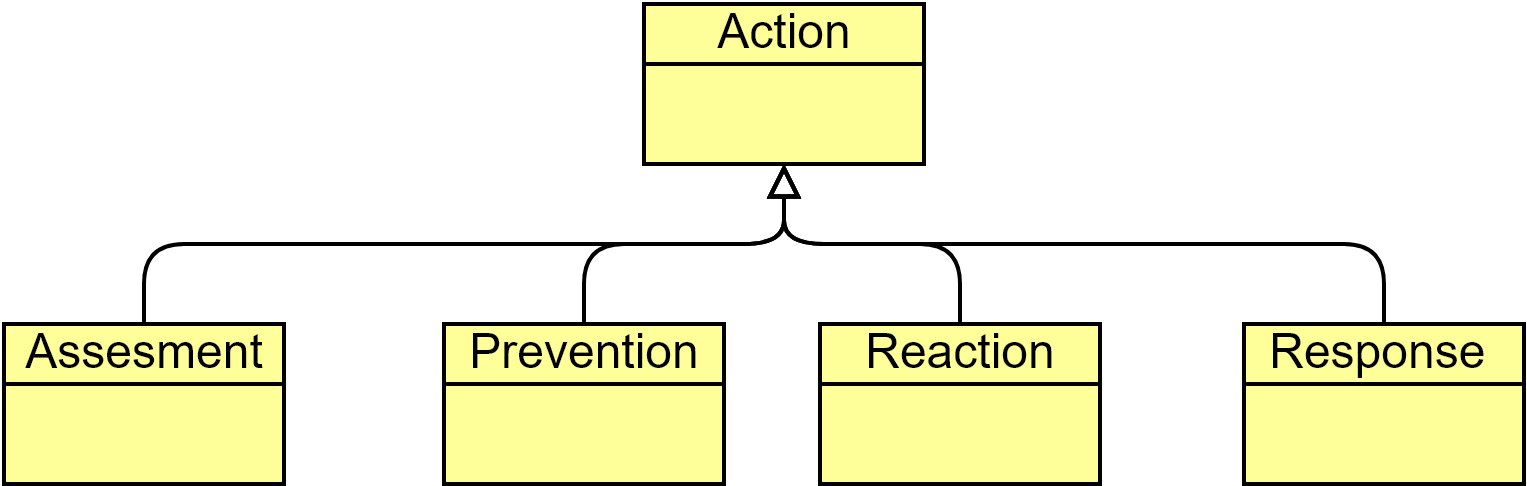
\includegraphics[width=4.36in,height=1.37in]{images/image6.png}
		\caption{Types of actions in a crisis}
		\label{fig:Types_of_actions_in_a_crisis}
	\end{Center}
\end{figure}
%%%%%%%%%%%%%%%%%%%% Figure/Image No: 1 Ends here %%%%%%%%%%%%%%%%%%%%
\end{Center}

``Action''  is a broad term covering all sorts of activities. Under it are depicted four classes of actions: the first two (on the left side of the diagram) are notably occurring before the crisis event happens. The other two (on the right side of the chart) apply to the aftermath. The depiction of the types of actions ordered sequentially along the temporal axis is depicted in Figure \ref{fig:Phases_in_crisis_management} where the crisis event takes a central place. 

\begin{Center}
%%%%%%%%%%%%%%%%%%%% Figure/Image No: 2 starts here %%%%%%%%%%%%%%%%%%%%

\begin{figure}[H]
	\begin{Center}
		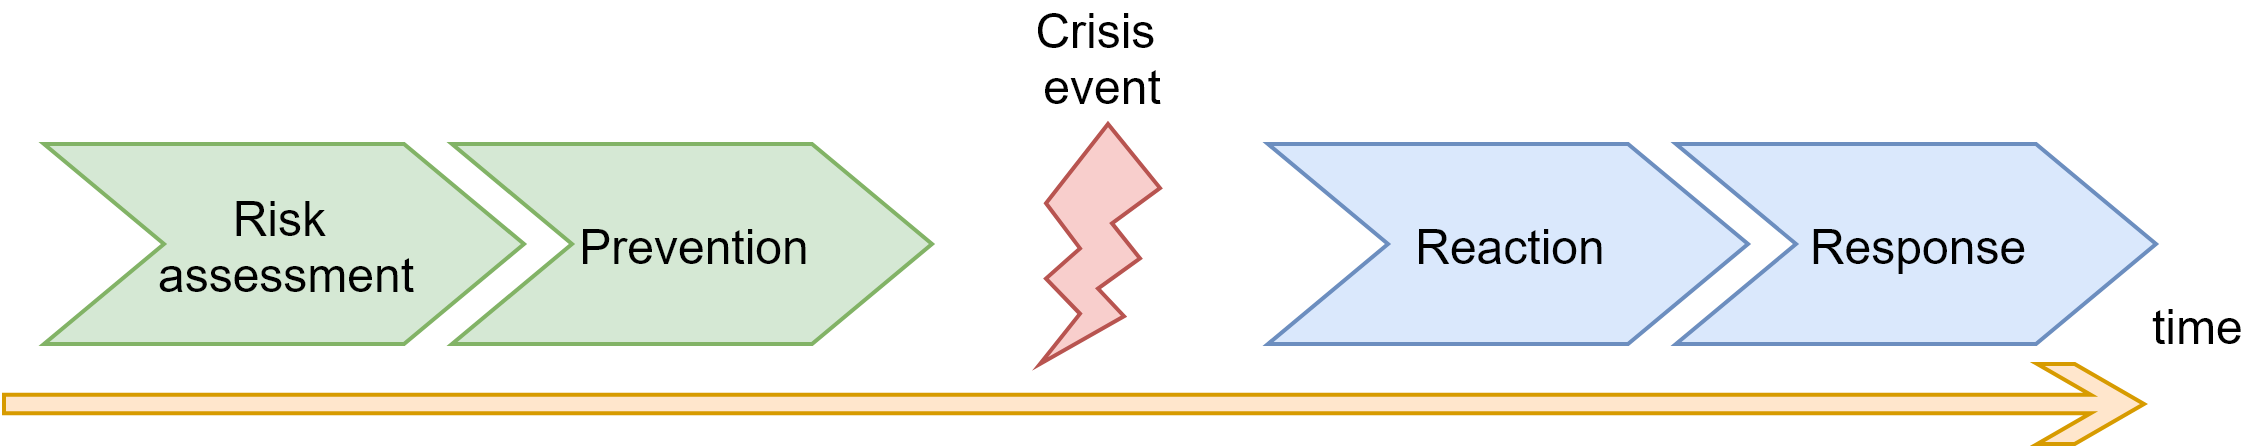
\includegraphics[width=\textwidth]{images/image4.png}
		\caption{Phases in crisis management}
		\label{fig:Phases_in_crisis_management}
	\end{Center}
\end{figure}
%%%%%%%%%%%%%%%%%%%% Figure/Image No: 2 Ends here %%%%%%%%%%%%%%%%%%%%
\end{Center}

The \textit{risk assessment} actions deal with risk identification, estimation of probability for each risk factor to occur. Also, at this stage is investigated the impact from the environmental, economic, social and public health perspectives, including who is impacted, how, and to what degree. 

The \textit{prevention} actions focus on what could be done to mitigate and alleviate the crisis impact in case it occurs. 

The \textit{crisis event} (or period) leads to an unstable and dangerous situation affecting an individual, group, or all of society. 

The \textit{reaction} actions deal with immediate mitigation while the \textit{responses} with medium to long-term mitigate the crisis consequences. These two action types: responses and reactions, which we collectively call \textit{measures}, and in our case \textit{measures to the COVID-19 crisis}, are the primary focus of the dataset. So, next, we define them in this context specifically. 

The \textit{COVID-19 reaction} is what an organisation plans to do to minimise the impact of the pandemics, such as including extra protective equipment for health workers, procurement of additional medical equipment, the introduction of social distancing, more rigorous border controls or their temporary closure. The reactions are actions related to the pandemic poses' health threats: ``a virus makes people sick, and something must be done about that'' . In addition to the pandemic consequences, the reactions have economic and social effects that can be directly observed or indirectly deduced. And so the reaction of the authorities to the virus affects the people too: consider, for example, the social distancing or the lockdown measures. We can say that the reactions are, in fact, to the health threat and that the main topics are anything related to health, pandemics, virus, infection etc. 

The \textit{COVID-19 responses} are measures set in place to compensate for the economic and social consequences of the pandemic crisis and diminish the effects of the authorities' reactions to the threat. Therefore the temporal horizon of the responses is much longer, and the topics they deal with are much broader and challenging to pinpoint. They could be anything related to social, economic, welfare, child care, telework, income support, increase in social protection and many other topics. 

Now, that the dataset domain is set to the COVID-19 reaction and response measures, with a predominant preference for the COVID-19 responses, we describe other criteria and provide some of our assumptions.  

\section{Criteria and assumptions about the data}
\label{sec:criteria}

\begin{itemize}
	\item Identify references to sources of data from discussions with the stakeholders and investigate them. From the selected ones collect text and metadata describing and classifying responses and reactions to the COVID-19 crisis. 
	\item To the extent possible, distinguish between reaction and response measures (as explained in Section \ref{sec:domain-delimitation}) because of the current project scope. 
	\item We assume that the official documents are a reliable source of measure descriptions.
	\item The primary focus is on collecting official texts of various registers (administrative, journalistic, legal, etc.) to enable further exercises to train machine learning models that can identify and distinguish a COVID-19 measure from other texts and, if possible, differences between the reactions and responses.
	\item Selecting the texts with these properties leads to a relatively scarce set of available resources. Therefore no (data) sampling was considered or any tests for the (data) balancing. Mainly we aimed at covering selected initial sources given the apparent degree of (data) representativeness to the semantic domain, which remains to be tested and analysed.
	\item We could identify two text registers (or genres) in the available sources, which is a valuable distinction in the further analysis. First is the journalistic or reportage style of language, which summarises and describes COVID-19 measures. Second is the legal style of language that characterises the source texts from where COVID-19 actions summaries are extracted. Possibly more genres could be identified in a detailed analysis. 
	\item Geographically, we select texts produced in the European Union, both at the EU level, by the institutions and at the member state level, by the national governments. 
	\item We select texts written in English as a first step and as an established limit to the scope, and later, in future work, this can be extended to texts written in the official EU 24 languages.
	\item We consider only texts issued after the beginning of 2020 when the COVID-19 pandemic started.

	\item A basic assumption is that Policy Watch Database (PWDB) is a suitable set of summarised descriptions of what a COVID-19 measure looks like. They cover broader economic and social issues in the area of working and living conditions and intentionally exclude COVID-19 reactions, which focus on public health-related issues. PWDB is a starting point and a pillar in developing this project. 
\end{itemize}

\section{Established data scope: how much is enough?}

Following an investigation and a series of discussions with the project stakeholders, it was decided to set the initial scope to collect data. This scope was set on pragmatic grounds with an awareness of possible extensions in future work.

This section presents the four datasets extracted from another source and constitute the current project dataset, Euro-COVID-19. The detailed description for each dataset is provided in a dedicated section below. Below is an outline of these datasets, along with their subcomponents. Note that the subcomponents are noteworthy at the level of this document to facilitate a deeper understanding of the data, but the dataset distributions merge them into usable wholes. We also provide a codified identifier for each dataset to allow for precise referencing.

\begin{itemize}
	\item \textbf{ds\_pwdb:} Policy Watch Dataset 
        \begin{itemize}
        	\item \textbf{what:} the content published on Eurofound website\footnote{ \href{https://www.eurofound.europa.eu/data/covid-19-eu-policywatch}{COVID-19 EU Policy Watch}}, that is enriched with content crawled from the referenced sources.
        	\item \textbf{why:} because it comprises a collection of manually authored documents summarising the COVID-19 response measures by the member states.
        \end{itemize}
	\item \textbf{ds\_eu\_cellar:} EU Cellar COVID-19 Dataset 
        \begin{itemize}
        	\item \textbf{what:} the EurLex\footnote{ \href{https://eur-lex.europa.eu/homepage.html}{EurLex: the portal to access European Union law} } documents fetched from Cellar\footnote{ \href{https://op.europa.eu/en/publication-detail/-/publication/50ecce27-857e-11e8-ac6a-01aa75ed71a1}{The semantic repository of the Publications Office} } marked with a special ``COVID-19'' tag. And, in addition, Cellar documents about selected EuroVoc\footnote{ \href{https://op.europa.eu/en/web/eu-vocabularies/dataset/-/resource?uri=http://publications.europa.eu/resource/dataset/eurovoc}{EuroVoc: The EU's Multilingual Thesaurus} } concepts (tightly related to COVID-19) dated after the 1st of January 2020.
        	\item \textbf{why:} because Cellar is the official EU semantic repository hosted by the Publications Office containing the official EU. documents. 
        \end{itemize}
	\item \textbf{ds\_eu\_timeline:} EU Action Timeline Dataset 
        \begin{itemize}
        	\item \textbf{what:} documents crawled from the EU action timeline website\footnote{ \href{https://ec.europa.eu/info/live-work-travel-eu/coronavirus-response/timeline-eu-action_en}{Timeline of EU action} }; and documents from the European Commission Press corner\footnote{ \href{https://ec.europa.eu/commission/presscorner/home/en}{Press material from the Commission Spokesperson's Service} } crawled by searching for selected EuroVoc concepts dated after 1st of January 2020.
        	\item \textbf{why:} because it comprises a curated list of official press releases on measures taken by the European Commission (the EU doer).
        \end{itemize}
	\item \textbf{ds\_ireland\_timeline:} Ireland COVID-19 Timeline Dataset
        \begin{itemize}
        	\item \textbf{what:} documents crawled from the Irish Government press corner by searching for pre-selected EuroVoc concepts dated after 1st of January 2020. 
        	\item \textbf{why:} it contains English language texts and constitutes an alternative source of (one) MS measures, which can be used to compare how ds\_pwdb covers a country. 
        \end{itemize}
\end{itemize}

\enlargethispage{1em}

The datasets listed above differ in terms of their internal structure and in terms of the content they cover. Each dataset will be presented in the sections below. A summary of the dataset content classification is provided in  Table \ref{tab:Classification of the dataset content}.

%%%%%%%%%%%%%%%%%%%% Table No: 2 starts here %%%%%%%%%%%%%%%%%%%%
\begin{table}[H]
 			\centering
\begin{tabular}{p{1.25in}p{1.25in}p{1.25in}p{1.25in}}
\hline
%row no:1
\multicolumn{1}{|p{1.25in}}{\Centering \textbf{@en}} & 
\multicolumn{1}{|p{1.25in}}{\Centering \textbf{EU}} & 
\multicolumn{1}{|p{1.25in}}{\Centering \textbf{MS (collectively)}} & 
\multicolumn{1}{|p{1.25in}|}{\Centering \textbf{MS (individual)}} \\
\hhline{----}
%row no:2
\multicolumn{1}{|p{1.25in}}{\Centering Journalistic text} & 
\multicolumn{1}{|p{1.25in}}{\Centering EU actions timeline} & 
\multicolumn{1}{|p{1.25in}}{\Centering Policy Watch DB} & 
\multicolumn{1}{|p{1.25in}|}{\Centering Ireland timeline} \\
\hhline{----}
%row no:3
\multicolumn{1}{|p{1.25in}}{\Centering Legal text} & 
\multicolumn{1}{|p{1.25in}}{\Centering EU Cellar COVID-19} & 
\multicolumn{1}{|p{1.25in}}{\Centering -} & 
\multicolumn{1}{|p{1.25in}|}{\Centering -} \\
\hhline{----}

\end{tabular}\caption{Classification of the dataset content}
\label{tab:Classification of the dataset content}
 \end{table}
\vspace{-1em}
%%%%%%%%%%%%%%%%%%% Table No: 2 ends here %%%%%%%%%%%%%%%%%%%%

In terms of content coverage, we distinguish datasets that cover: the EU measures, the MS measures for all EU states in a single collection, the MS measures segregated for each country. 

In terms of language register\footnote{Register (in Sociolinguistics) is a variety of language used for a particular purpose or in a particular communicative situation. This term is remotely synonym to text type, style and genre.} two major ones are identified that characterise existent texts: (a) \textit{Journalistic or reportage text register} and (b) \textit{formal administrative and legal text register}. The aim here is not to describe these registers but merely identify them as making such a distinction may be of significant relevance in the data analysis phase. 

Datasets pertaining to the journalistic(reportage) text register are

\begin{itemize}
	\item Policy Watch Database 
	\item EU action timeline

	\item Ireland action timeline
\end{itemize}

In the formal administrative and legal text register fall the following datasets

\begin{itemize}
	\item EU Cellar COVID-19 
\end{itemize}

In the next section we proceed with describing the structure for each dataset and some of its peculiarities.

\section{Dataset description: what is inside? }

This section describes the datasets in terms of their structure, scope and manner in which the data have been collected. 

\subsection{Policy watch database (ds\_pwdb)}

Eurofound's COVID-19 EU PolicyWatch (PWDB)\footnote{ PWDB download page  } collates information on the responses of government and social partners to the crisis, as well as gathering examples of company practices aimed at mitigating the social and economic impacts. Data has been mainly provided by the Network of Eurofound Correspondents, with quality control carried out by Eurofound staff.

PWDB includes large-scale government measures and wider collective agreements, as well as regional and local initiatives and support measures for smaller groups of workers. As the situation is evolving, measures are newly implemented, changed or cancelled and replaced at rapid speed. It is planned to update the cases with information on the actual uptake of the main measures. Outside the scope of this database are public health measures, travel and movement restrictions and company-specific job losses. 

The original PWDB contains a rich set of attributes. Only a subset is considered relevant from the business perspective to the current project and is listed in the table below. The original structure is transformed into a simplified form for harmonisation with other datasets and easier usage. The data structure of the transformed core PWDB dataset (ds\_pwdb\_core) is described in Table \ref{tab:dspwdbcore}.

In column BF are provided references to the business features for each data attribute. However, it is not always possible to establish a reliable one to one mapping. Therefore, in some places, we use: the tilde sign ($\sim$) to signify an approximate relation, the plus sign to signify that more than one BF is included or represented by the data attribute.

%%%%%%%%%%%%%%%%%%%% Table No: 3 starts here %%%%%%%%%%%%%%%%%%%%
{
\setlength\extrarowheight{3pt}
\begin{longtable}{p{1.16in}p{3.48in}p{0.62in}}

\endfirsthead
\multicolumn{3}{c}{\textit{continued from previous page}}%\hline
\endhead
\multicolumn{3}{r}{\textit{continued on next page}} \\
\endfoot
\endlastfoot\hline
%row no:1
\multicolumn{1}{|p{1.16in}}{\textbf{Data attribute}} & 
\multicolumn{1}{|p{3.48in}}{\textbf{Description}} & 
\multicolumn{1}{|p{0.62in}|}{\textbf{BF}} \\
\hhline{---}
%row no:2
\multicolumn{1}{|p{1.16in}}{Category} & 
\multicolumn{1}{|p{3.48in}}{Nine\ high-level categories for grouping the COVID-19 measures  (proposed by the EuroFond team\footnote{ About Eurofound }).} & 
\multicolumn{1}{|p{0.62in}|}{BF2} \\
\hhline{---}
%row no:3
\multicolumn{1}{|p{1.16in}}{Subcategory} & 
\multicolumn{1}{|p{3.48in}}{Further categorisation into fine grained categories, under a parent category. The two level taxonomy is not documented here but can be recreated from the dataset. } & 
\multicolumn{1}{|p{0.62in}|}{BF2} \\
\hhline{---}
%row no:4
\multicolumn{1}{|p{1.16in}}{Target group (L1)} & 
\multicolumn{1}{|p{3.48in}}{The database provides target groups for each measure. Target groups are organised on two levels: L1 $\&$  L2. The L1 level broadly differentiates between \textit{workers, businesses} and \textit{citizens}.} & 
\multicolumn{1}{|p{0.62in}|}{BF8} \\
\hhline{---}
%row no:5
\multicolumn{1}{|p{1.16in}}{Target group (L2)} & 
\multicolumn{1}{|p{3.48in}}{The L2 level contains more fine grained distinctions containing 42 specific target groups distinctions in total, including for example: \par \begin{itemize}
	\item Workers: \href{https://static.Eurofound.europa.eu/COVID-19db/targetGroups/self-employed.html}{\textcolor[HTML]{1155CC}{\ul{Self-employed}}}, \href{https://static.Eurofound.europa.eu/COVID-19db/targetGroups/seasonal_workers.html}{\textcolor[HTML]{1155CC}{\ul{Seasonal workers}}}, \href{https://static.Eurofound.europa.eu/COVID-19db/targetGroups/platform_workers.html}{\textcolor[HTML]{1155CC}{\ul{Platform workers}}}, etc. \par 	\item Businesses: \href{https://static.Eurofound.europa.eu/COVID-19db/targetGroups/smes.html}{\textcolor[HTML]{1155CC}{\ul{SMEs}}}, \href{https://static.Eurofound.europa.eu/COVID-19db/targetGroups/start-ups.html}{\textcolor[HTML]{1155CC}{\ul{Start-ups}}}, \href{https://static.Eurofound.europa.eu/COVID-19db/targetGroups/larger_corporations.html}{\textcolor[HTML]{1155CC}{\ul{Larger corporations}}}, etc. \par 	\item Citizens: \href{https://static.Eurofound.europa.eu/COVID-19db/targetGroups/parents.html}{\textcolor[HTML]{1155CC}{\ul{Parents}}}, \href{https://static.Eurofound.europa.eu/COVID-19db/targetGroups/older_citizens.html}{\textcolor[HTML]{1155CC}{\ul{Older citizens}}}, \href{https://static.Eurofound.europa.eu/COVID-19db/targetGroups/migrants.html}{\textcolor[HTML]{1155CC}{\ul{Migrants}}}, etc.
\end{itemize}} & 
\multicolumn{1}{|p{0.62in}|}{BF8} \\
\hhline{---}
%row no:6
\multicolumn{1}{|p{1.16in}}{Country} & 
\multicolumn{1}{|p{3.48in}}{The country where the COVID-19 measure is adopted by the government and social partners.} & 
\multicolumn{1}{|p{0.62in}|}{BF5, BF1} \\
\hhline{---}
%row no:7
\multicolumn{1}{|p{1.16in}}{Involved actors} & 
\multicolumn{1}{|p{3.48in}}{Eurofound identified 757 legislations and other statutory regulations, 452 of which have been created entirely in the context of COVID-19. This section gives an overview of social partner's involvement in designing and implementing these measures.} & 
\multicolumn{1}{|p{0.62in}|}{$ \sim $  (BF1 + BF8)} \\
\hhline{---}
%row no:8
\multicolumn{1}{|p{1.16in}}{Funding} & 
\multicolumn{1}{|p{3.48in}}{The sources of financing the measure, if the measure involves financial expenditures. Some measures do not have fundings. } & 
\multicolumn{1}{|p{0.62in}|}{$ \sim $  BF6} \\
\hhline{---}
%row no:9
\multicolumn{1}{|p{1.16in}}{Type} & 
\multicolumn{1}{|p{3.48in}}{Classification of the document types from where the description of the measures originates. Six types of source documents are distinguished, including legislations, collective agreements, recommendations and company practices.} & 
\multicolumn{1}{|p{0.62in}|}{} \\
\hhline{---}
%row no:10
\multicolumn{1}{|p{1.16in}}{Start $\&$  End dates} & 
\multicolumn{1}{|p{3.48in}}{The time period when the measure is applied.} & 
\multicolumn{1}{|p{0.62in}|}{BF4} \\
\hhline{---}
%row no:11
\multicolumn{1}{|p{1.16in}}{Creation date} & 
\multicolumn{1}{|p{3.48in}}{When the measure entry was created in the database.} & 
\multicolumn{1}{|p{0.62in}|}{$ \sim $  BF3} \\
\hhline{---}
%row no:12
\multicolumn{1}{|p{1.16in}}{Update date} & 
\multicolumn{1}{|p{3.48in}}{When last changes were made to the measure entry description.} & 
\multicolumn{1}{|p{0.62in}|}{$ \sim $  BF3} \\
\hhline{---}
%row no:13
\multicolumn{1}{|p{1.16in}}{Background information} & 
\multicolumn{1}{|p{3.48in}}{A short text providing the context and background information useful to understand the measure description.} & 
\multicolumn{1}{|p{0.62in}|}{BF10} \\
\hhline{---}
%row no:14
\multicolumn{1}{|p{1.16in}}{Content of measure} & 
\multicolumn{1}{|p{3.48in}}{A short text representing the abstract or a concise description of the measure.} & 
\multicolumn{1}{|p{0.62in}|}{BF10} \\
\hhline{---}
%row no:15
\multicolumn{1}{|p{1.16in}}{Content updates} & 
\multicolumn{1}{|p{3.48in}}{Short updates to the content of the measure.} & 
\multicolumn{1}{|p{0.62in}|}{BF10} \\
\hhline{---}
%row no:16
\multicolumn{1}{|p{1.16in}}{Use of measure} & 
\multicolumn{1}{|p{3.48in}}{Information about the results and outcomes of executing/enacting the measure.} & 
\multicolumn{1}{|p{0.62in}|}{BF10} \\
\hhline{---}
%row no:17
\multicolumn{1}{|p{1.16in}}{Title} & 
\multicolumn{1}{|p{3.48in}}{A short text used to identify the measure, place it in context, and convey a minimal summary of its contents.} & 
\multicolumn{1}{|p{0.62in}|}{BF10} \\
\hhline{---}
\caption{The attribute structure for core PWDB dataset (ds\_pwdb\_core)}
\label{tab:dspwdbcore}
\end{longtable}}



%%%%%%%%%%%%%%%%%%%% Table No: 3 ends here %%%%%%%%%%%%%%%%%%%%

In the core dataset, a list of source references is provided. They represent links to the original documents elaborating on the contents of the measure. We proceeded with downloading, cleaning and injecting the content of the sources into the PWD dataset, this way extending it.  
An additional set of data attributes is provided in the extended version of the PWDB dataset, as is listed in  Table \ref{tab:dspwdbext)}.

%%%%%%%%%%%%%%%%%%%% Table No: 4 starts here %%%%%%%%%%%%%%%%%%%%
\begin{table}[H]
 			\centering
\begin{tabular}{p{1.04in}p{4.24in}p{0.39in}}
\hline
%row no:1
\multicolumn{1}{|p{1.04in}}{\textbf{Data attribute}} & 
\multicolumn{1}{|p{4.24in}}{\textbf{Description}} & 
\multicolumn{1}{|p{0.39in}|}{\textbf{BF}} \\
\hhline{---}
%row no:2
\multicolumn{1}{|p{1.04in}}{Source URL} & 
\multicolumn{1}{|p{4.24in}}{The measure descriptions are based on external sources referenced by URLs} & 
\multicolumn{1}{|p{0.39in}|}{} \\
\hhline{---}
%row no:3
\multicolumn{1}{|p{1.04in}}{Source content} & 
\multicolumn{1}{|p{4.24in}}{The content (in simple text) downloaded by accessing the document at the source URL.} & 
\multicolumn{1}{|p{0.39in}|}{BF10} \\
\hhline{---}
%row no:4
\multicolumn{1}{|p{1.04in}}{Source title} & 
\multicolumn{1}{|p{4.24in}}{The title of the source document, if possible to retrieve} & 
\multicolumn{1}{|p{0.39in}|}{BF10} \\
\hhline{---}
%row no:5
\multicolumn{1}{|p{1.04in}}{Source language} & 
\multicolumn{1}{|p{4.24in}}{The language of the source content is determined by a language identification system.} & 
\multicolumn{1}{|p{0.39in}|}{} \\
\hhline{---}

\end{tabular}
\caption{The additional set of attributes constituting the PWBD extension (ds\_pwdb\_ext)}
\label{tab:dspwdbext)}
\end{table}
%%%%%%%%%%%%%%%%%%%% Table No: 4 ends here %%%%%%%%%%%%%%%%%%%%

Finally, the core and the extended dataset variants are merged and provided as a unified PWDB dataset. 

\enlargethispage{1em}

\subsection{EU Cellar COVID-19 dataset (ds\_eu\_cellar)}

The Cellar is the semantic repository of the Publications Office. It stores essential legal documents, general publications and other vital EU level documents. We query this repository to construct the EU level COVID-19 datasets containing the document content and the associated metadata. 

In the context of the current exercise, we distinguish the core and the extended datasets variants, which are results of querying Cellar with two different SPARQL queries.

The core dataset is the result of querying for documents (called works) that are annotated with a special ``COVID-19''  tag in the Cellar repository. The tagging is performed manually by the EurLex team and its contractors. This tag marks documents that have been identified as dealing directly with issues of the COVID-19 pandemic. 

The extended dataset is also the result of querying for documents (called works) in Cellar, which are annotated with any of the pre-selected EuroVoc concepts. We have manually selected concepts from the EuroVoc thesaurus judging whether a concept is or is not relevant to the COVID-19 pandemics. The relevance criteria covers both: the reaction topics, those pertaining to the public health domain, and the response topics, those pertaining to broader social and economic domains (for domain delineation see Section \ref{sec:domain-delimitation} ). The list of selected EuroVoc concepts is provided in  Table \ref{tab:EuroVoc concepts considered highly relevant for COVID-19 document search}. 

%%%%%%%%%%%%%%%%%%%% Table No: 5 starts here %%%%%%%%%%%%%%%%%%%%
{
\setlength\extrarowheight{3pt}
\begin{longtable}{p{2.5in}p{2.96in}}

\endfirsthead
\multicolumn{2}{c}{\textit{continued from previous page}} %\hline
\endhead
\multicolumn{2}{r}{\textit{continued on next page}} \\
\endfoot
\endlastfoot\hline
%row no:1
\multicolumn{1}{|p{2.5in}}{\textbf{Concept URI}} & 
\multicolumn{1}{|p{2.96in}|}{\textbf{Concept preferred label}} \\
\hhline{--}
%row no:2
\multicolumn{1}{|p{2.5in}}{{\fontsize{10pt}{12.0pt}\selectfont http://eurovoc.europa.eu/1005}} & 
\multicolumn{1}{|p{2.96in}|}{{\fontsize{10pt}{12.0pt}\selectfont EU financing}} \\
\hhline{--}
%row no:3
\multicolumn{1}{|p{2.5in}}{{\fontsize{10pt}{12.0pt}\selectfont http://eurovoc.europa.eu/1439}} & 
\multicolumn{1}{|p{2.96in}|}{{\fontsize{10pt}{12.0pt}\selectfont innovation}} \\
\hhline{--}
%row no:4
\multicolumn{1}{|p{2.5in}}{{\fontsize{10pt}{12.0pt}\selectfont http://eurovoc.europa.eu/1633}} & 
\multicolumn{1}{|p{2.96in}|}{{\fontsize{10pt}{12.0pt}\selectfont free movement of persons}} \\
\hhline{--}
%row no:5
\multicolumn{1}{|p{2.5in}}{{\fontsize{10pt}{12.0pt}\selectfont http://eurovoc.europa.eu/1754}} & 
\multicolumn{1}{|p{2.96in}|}{{\fontsize{10pt}{12.0pt}\selectfont illness}} \\
\hhline{--}
%row no:6
\multicolumn{1}{|p{2.5in}}{{\fontsize{10pt}{12.0pt}\selectfont http://eurovoc.europa.eu/1756}} & 
\multicolumn{1}{|p{2.96in}|}{{\fontsize{10pt}{12.0pt}\selectfont respiratory disease}} \\
\hhline{--}
%row no:7
\multicolumn{1}{|p{2.5in}}{{\fontsize{10pt}{12.0pt}\selectfont http://eurovoc.europa.eu/1759}} & 
\multicolumn{1}{|p{2.96in}|}{{\fontsize{10pt}{12.0pt}\selectfont infectious disease}} \\
\hhline{--}
%row no:8
\multicolumn{1}{|p{2.5in}}{{\fontsize{10pt}{12.0pt}\selectfont http://eurovoc.europa.eu/1802}} & 
\multicolumn{1}{|p{2.96in}|}{{\fontsize{10pt}{12.0pt}\selectfont labour market}} \\
\hhline{--}
%row no:9
\multicolumn{1}{|p{2.5in}}{{\fontsize{10pt}{12.0pt}\selectfont http://eurovoc.europa.eu/1854}} & 
\multicolumn{1}{|p{2.96in}|}{{\fontsize{10pt}{12.0pt}\selectfont disease prevention}} \\
\hhline{--}
%row no:10
\multicolumn{1}{|p{2.5in}}{{\fontsize{10pt}{12.0pt}\selectfont http://eurovoc.europa.eu/192}} & 
\multicolumn{1}{|p{2.96in}|}{{\fontsize{10pt}{12.0pt}\selectfont health control}} \\
\hhline{--}
%row no:11
\multicolumn{1}{|p{2.5in}}{{\fontsize{10pt}{12.0pt}\selectfont http://eurovoc.europa.eu/2916}} & 
\multicolumn{1}{|p{2.96in}|}{{\fontsize{10pt}{12.0pt}\selectfont applied research}} \\
\hhline{--}
%row no:12
\multicolumn{1}{|p{2.5in}}{{\fontsize{10pt}{12.0pt}\selectfont http://eurovoc.europa.eu/2923}} & 
\multicolumn{1}{|p{2.96in}|}{{\fontsize{10pt}{12.0pt}\selectfont medical research}} \\
\hhline{--}
%row no:13
\multicolumn{1}{|p{2.5in}}{{\fontsize{10pt}{12.0pt}\selectfont http://eurovoc.europa.eu/3730}} & 
\multicolumn{1}{|p{2.96in}|}{{\fontsize{10pt}{12.0pt}\selectfont health risk}} \\
\hhline{--}
%row no:14
\multicolumn{1}{|p{2.5in}}{{\fontsize{10pt}{12.0pt}\selectfont http://eurovoc.europa.eu/3885}} & 
\multicolumn{1}{|p{2.96in}|}{{\fontsize{10pt}{12.0pt}\selectfont public health}} \\
\hhline{--}
%row no:15
\multicolumn{1}{|p{2.5in}}{{\fontsize{10pt}{12.0pt}\selectfont http://eurovoc.europa.eu/4470}} & 
\multicolumn{1}{|p{2.96in}|}{{\fontsize{10pt}{12.0pt}\selectfont tourism}} \\
\hhline{--}
%row no:16
\multicolumn{1}{|p{2.5in}}{{\fontsize{10pt}{12.0pt}\selectfont http://eurovoc.europa.eu/4505}} & 
\multicolumn{1}{|p{2.96in}|}{{\fontsize{10pt}{12.0pt}\selectfont air transport}} \\
\hhline{--}
%row no:17
\multicolumn{1}{|p{2.5in}}{{\fontsize{10pt}{12.0pt}\selectfont http://eurovoc.europa.eu/5237}} & 
\multicolumn{1}{|p{2.96in}|}{{\fontsize{10pt}{12.0pt}\selectfont research and development}} \\
\hhline{--}
%row no:18
\multicolumn{1}{|p{2.5in}}{{\fontsize{10pt}{12.0pt}\selectfont http://eurovoc.europa.eu/835}} & 
\multicolumn{1}{|p{2.96in}|}{{\fontsize{10pt}{12.0pt}\selectfont aid to undertakings}} \\
\hhline{--}
%row no:19
\multicolumn{1}{|p{2.5in}}{{\fontsize{10pt}{12.0pt}\selectfont http://eurovoc.europa.eu/1280}} & 
\multicolumn{1}{|p{2.96in}|}{{\fontsize{10pt}{12.0pt}\selectfont occupational health}} \\
\hhline{--}
%row no:20
\multicolumn{1}{|p{2.5in}}{{\fontsize{10pt}{12.0pt}\selectfont http://eurovoc.europa.eu/1634}} & 
\multicolumn{1}{|p{2.96in}|}{{\fontsize{10pt}{12.0pt}\selectfont free movement of workers}} \\
\hhline{--}
%row no:21
\multicolumn{1}{|p{2.5in}}{{\fontsize{10pt}{12.0pt}\selectfont http://eurovoc.europa.eu/2062}} & 
\multicolumn{1}{|p{2.96in}|}{{\fontsize{10pt}{12.0pt}\selectfont standard of living}} \\
\hhline{--}
%row no:22
\multicolumn{1}{|p{2.5in}}{{\fontsize{10pt}{12.0pt}\selectfont http://eurovoc.europa.eu/2479}} & 
\multicolumn{1}{|p{2.96in}|}{{\fontsize{10pt}{12.0pt}\selectfont health policy}} \\
\hhline{--}
%row no:23
\multicolumn{1}{|p{2.5in}}{{\fontsize{10pt}{12.0pt}\selectfont http://eurovoc.europa.eu/5891}} & 
\multicolumn{1}{|p{2.96in}|}{{\fontsize{10pt}{12.0pt}\selectfont public awareness campaign}} \\
\hhline{--}
%row no:24
\multicolumn{1}{|p{2.5in}}{{\fontsize{10pt}{12.0pt}\selectfont http://eurovoc.europa.eu/82}} & 
\multicolumn{1}{|p{2.96in}|}{{\fontsize{10pt}{12.0pt}\selectfont working conditions}} \\
\hhline{--}
%row no:25
\multicolumn{1}{|p{2.5in}}{{\fontsize{10pt}{12.0pt}\selectfont http://eurovoc.europa.eu/2473}} & 
\multicolumn{1}{|p{2.96in}|}{{\fontsize{10pt}{12.0pt}\selectfont communications policy}} \\
\hhline{--}
%row no:26
\multicolumn{1}{|p{2.5in}}{{\fontsize{10pt}{12.0pt}\selectfont http://eurovoc.europa.eu/3086}} & 
\multicolumn{1}{|p{2.96in}|}{{\fontsize{10pt}{12.0pt}\selectfont economic consequence}} \\
\hhline{--}
%row no:27
\multicolumn{1}{|p{2.5in}}{{\fontsize{10pt}{12.0pt}\selectfont http://eurovoc.europa.eu/4636}} & 
\multicolumn{1}{|p{2.96in}|}{{\fontsize{10pt}{12.0pt}\selectfont vaccination}} \\
\hhline{--}
%row no:28
\multicolumn{1}{|p{2.5in}}{{\fontsize{10pt}{12.0pt}\selectfont http://eurovoc.europa.eu/5992}} & 
\multicolumn{1}{|p{2.96in}|}{{\fontsize{10pt}{12.0pt}\selectfont economic activity}} \\
\hhline{--}
%row no:29
\multicolumn{1}{|p{2.5in}}{{\fontsize{10pt}{12.0pt}\selectfont http://eurovoc.europa.eu/712}} & 
\multicolumn{1}{|p{2.96in}|}{{\fontsize{10pt}{12.0pt}\selectfont economic support}} \\
\hhline{--}
%row no:30
\multicolumn{1}{|p{2.5in}}{{\fontsize{10pt}{12.0pt}\selectfont http://eurovoc.europa.eu/826}} & 
\multicolumn{1}{|p{2.96in}|}{{\fontsize{10pt}{12.0pt}\selectfont aid to disadvantaged groups}} \\
\hhline{--}
%row no:31
\multicolumn{1}{|p{2.5in}}{{\fontsize{10pt}{12.0pt}\selectfont http://eurovoc.europa.eu/1596}} & 
\multicolumn{1}{|p{2.96in}|}{{\fontsize{10pt}{12.0pt}\selectfont health legislation}} \\
\hhline{--}
%row no:32
\multicolumn{1}{|p{2.5in}}{{\fontsize{10pt}{12.0pt}\selectfont http://eurovoc.europa.eu/2870}} & 
\multicolumn{1}{|p{2.96in}|}{{\fontsize{10pt}{12.0pt}\selectfont quality of life}} \\
\hhline{--}
%row no:33
\multicolumn{1}{|p{2.5in}}{{\fontsize{10pt}{12.0pt}\selectfont http://eurovoc.europa.eu/3956}} & 
\multicolumn{1}{|p{2.96in}|}{{\fontsize{10pt}{12.0pt}\selectfont social sciences}} \\
\hhline{--}
%row no:34
\multicolumn{1}{|p{2.5in}}{{\fontsize{10pt}{12.0pt}\selectfont http://eurovoc.europa.eu/899}} & 
\multicolumn{1}{|p{2.96in}|}{{\fontsize{10pt}{12.0pt}\selectfont economic aid}} \\
\hhline{--}
%row no:35
\multicolumn{1}{|p{2.5in}}{{\fontsize{10pt}{12.0pt}\selectfont http://eurovoc.europa.eu/7983}} & 
\multicolumn{1}{|p{2.96in}|}{{\fontsize{10pt}{12.0pt}\selectfont European Centre for Disease Prevention and Control}} \\
\hhline{--}
%row no:36
\multicolumn{1}{|p{2.5in}}{{\fontsize{10pt}{12.0pt}\selectfont http://eurovoc.europa.eu/83}} & 
\multicolumn{1}{|p{2.96in}|}{{\fontsize{10pt}{12.0pt}\selectfont living conditions}} \\
\hhline{--}
%row no:37
\multicolumn{1}{|p{2.5in}}{{\fontsize{10pt}{12.0pt}\selectfont http://eurovoc.europa.eu/85}} & 
\multicolumn{1}{|p{2.96in}|}{{\fontsize{10pt}{12.0pt}\selectfont social situation}} \\
\hhline{--}
%row no:38
\multicolumn{1}{|p{2.5in}}{{\fontsize{10pt}{12.0pt}\selectfont http://eurovoc.europa.eu/5764}} & 
\multicolumn{1}{|p{2.96in}|}{{\fontsize{10pt}{12.0pt}\selectfont organisation of health care}} \\
\hhline{--}
%row no:39
\multicolumn{1}{|p{2.5in}}{{\fontsize{10pt}{12.0pt}\selectfont http://eurovoc.europa.eu/3552}} & 
\multicolumn{1}{|p{2.96in}|}{{\fontsize{10pt}{12.0pt}\selectfont teleworking}} \\
\hhline{--}
%row no:40
\multicolumn{1}{|p{2.5in}}{{\fontsize{10pt}{12.0pt}\selectfont http://eurovoc.europa.eu/1742}} & 
\multicolumn{1}{|p{2.96in}|}{{\fontsize{10pt}{12.0pt}\selectfont job preservation}} \\
\hhline{--}
%row no:41
\multicolumn{1}{|p{2.5in}}{{\fontsize{10pt}{12.0pt}\selectfont http://eurovoc.europa.eu/886}} & 
\multicolumn{1}{|p{2.96in}|}{{\fontsize{10pt}{12.0pt}\selectfont state of emergency}} \\
\hhline{--}
%row no:42
\multicolumn{1}{|p{2.5in}}{{\fontsize{10pt}{12.0pt}\selectfont http://eurovoc.europa.eu/1926}} & 
\multicolumn{1}{|p{2.96in}|}{{\fontsize{10pt}{12.0pt}\selectfont working environment}} \\
\hhline{--}
%row no:43
\multicolumn{1}{|p{2.5in}}{{\fontsize{10pt}{12.0pt}\selectfont http://eurovoc.europa.eu/4116}} & 
\multicolumn{1}{|p{2.96in}|}{{\fontsize{10pt}{12.0pt}\selectfont health service}} \\
\hhline{--}
%row no:44
\multicolumn{1}{|p{2.5in}}{{\fontsize{10pt}{12.0pt}\selectfont http://eurovoc.europa.eu/5612}} & 
\multicolumn{1}{|p{2.96in}|}{{\fontsize{10pt}{12.0pt}\selectfont protective equipment}} \\
\hhline{--}
%row no:45
\multicolumn{1}{|p{2.5in}}{{\fontsize{10pt}{12.0pt}\selectfont http://eurovoc.europa.eu/837}} & 
\multicolumn{1}{|p{2.96in}|}{{\fontsize{10pt}{12.0pt}\selectfont epidemic}} \\
\hhline{--}
%row no:46
\multicolumn{1}{|p{2.5in}}{{\fontsize{10pt}{12.0pt}\selectfont http://eurovoc.europa.eu/2270}} & 
\multicolumn{1}{|p{2.96in}|}{{\fontsize{10pt}{12.0pt}\selectfont social participation}} \\
\hhline{--}
%row no:47
\multicolumn{1}{|p{2.5in}}{{\fontsize{10pt}{12.0pt}\selectfont http://eurovoc.europa.eu/838}} & 
\multicolumn{1}{|p{2.96in}|}{{\fontsize{10pt}{12.0pt}\selectfont epidemiology}} \\
\hhline{--}
%row no:48
\multicolumn{1}{|p{2.5in}}{{\fontsize{10pt}{12.0pt}\selectfont http://eurovoc.europa.eu/2793}} & 
\multicolumn{1}{|p{2.96in}|}{{\fontsize{10pt}{12.0pt}\selectfont aid programme}} \\
\hhline{--}
%row no:49
\multicolumn{1}{|p{2.5in}}{{\fontsize{10pt}{12.0pt}\selectfont http://eurovoc.europa.eu/3588}} & 
\multicolumn{1}{|p{2.96in}|}{{\fontsize{10pt}{12.0pt}\selectfont restriction of liberty}} \\
\hhline{--}
%row no:50
\multicolumn{1}{|p{2.5in}}{{\fontsize{10pt}{12.0pt}\selectfont http://eurovoc.europa.eu/6781}} & 
\multicolumn{1}{|p{2.96in}|}{{\fontsize{10pt}{12.0pt}\selectfont basic needs}} \\
\hhline{--}
%row no:51
\multicolumn{1}{|p{2.5in}}{{\fontsize{10pt}{12.0pt}\selectfont http://eurovoc.europa.eu/3371}} & 
\multicolumn{1}{|p{2.96in}|}{{\fontsize{10pt}{12.0pt}\selectfont public hygiene}} \\
\hhline{--}
%row no:52
\multicolumn{1}{|p{2.5in}}{{\fontsize{10pt}{12.0pt}\selectfont http://eurovoc.europa.eu/2013}} & 
\multicolumn{1}{|p{2.96in}|}{{\fontsize{10pt}{12.0pt}\selectfont mass media}} \\
\hhline{--}
%row no:53
\multicolumn{1}{|p{2.5in}}{{\fontsize{10pt}{12.0pt}\selectfont http://eurovoc.europa.eu/7131}} & 
\multicolumn{1}{|p{2.96in}|}{{\fontsize{10pt}{12.0pt}\selectfont social impact}} \\
\hhline{--}
%row no:54
\multicolumn{1}{|p{2.5in}}{{\fontsize{10pt}{12.0pt}\selectfont http://eurovoc.europa.eu/3906}} & 
\multicolumn{1}{|p{2.96in}|}{{\fontsize{10pt}{12.0pt}\selectfont freedom of movement}} \\
\hhline{--}
%row no:55
\multicolumn{1}{|p{2.5in}}{{\fontsize{10pt}{12.0pt}\selectfont http://eurovoc.europa.eu/3370}} & 
\multicolumn{1}{|p{2.96in}|}{{\fontsize{10pt}{12.0pt}\selectfont patient rights}} \\
\hhline{--}
%row no:56
\multicolumn{1}{|p{2.5in}}{{\fontsize{10pt}{12.0pt}\selectfont http://eurovoc.europa.eu/4881}} & 
\multicolumn{1}{|p{2.96in}|}{{\fontsize{10pt}{12.0pt}\selectfont social well-being}} \\
\hhline{--}
%row no:57
\multicolumn{1}{|p{2.5in}}{{\fontsize{10pt}{12.0pt}\selectfont http://eurovoc.europa.eu/86}} & 
\multicolumn{1}{|p{2.96in}|}{{\fontsize{10pt}{12.0pt}\selectfont socioeconomic conditions}} \\
\hhline{--}
%row no:58
\multicolumn{1}{|p{2.5in}}{{\fontsize{10pt}{12.0pt}\selectfont http://eurovoc.europa.eu/1758}} & 
\multicolumn{1}{|p{2.96in}|}{{\fontsize{10pt}{12.0pt}\selectfont endemic disease}} \\
\hhline{--}
%row no:59
\multicolumn{1}{|p{2.5in}}{{\fontsize{10pt}{12.0pt}\selectfont http://eurovoc.europa.eu/779}} & 
\multicolumn{1}{|p{2.96in}|}{{\fontsize{10pt}{12.0pt}\selectfont distance learning}} \\
\hhline{--}
%row no:60
\multicolumn{1}{|p{2.5in}}{{\fontsize{10pt}{12.0pt}\selectfont http://eurovoc.europa.eu/6609}} & 
\multicolumn{1}{|p{2.96in}|}{{\fontsize{10pt}{12.0pt}\selectfont self-regulation}} \\
\hhline{--}
%row no:61
\multicolumn{1}{|p{2.5in}}{{\fontsize{10pt}{12.0pt}\selectfont http://eurovoc.europa.eu/6770}} & 
\multicolumn{1}{|p{2.96in}|}{{\fontsize{10pt}{12.0pt}\selectfont disinformation}} \\
\hhline{--}
%row no:62
\multicolumn{1}{|p{2.5in}}{{\fontsize{10pt}{12.0pt}\selectfont http://eurovoc.europa.eu/c\_324b44f1}} & 
\multicolumn{1}{|p{2.96in}|}{{\fontsize{10pt}{12.0pt}\selectfont social media}} \\
\hhline{--}
%row no:63
\multicolumn{1}{|p{2.5in}}{{\fontsize{10pt}{12.0pt}\selectfont http://eurovoc.europa.eu/c\_5b447e3a}} & 
\multicolumn{1}{|p{2.96in}|}{{\fontsize{10pt}{12.0pt}\selectfont crisis management}} \\
\hhline{--}
%row no:64
\multicolumn{1}{|p{2.5in}}{{\fontsize{10pt}{12.0pt}\selectfont http://eurovoc.europa.eu/c\_31da5694}} & 
\multicolumn{1}{|p{2.96in}|}{{\fontsize{10pt}{12.0pt}\selectfont e-Health}} \\
\hhline{--}
%row no:65
\multicolumn{1}{|p{2.5in}}{{\fontsize{10pt}{12.0pt}\selectfont http://eurovoc.europa.eu/c\_60d3928d}} & 
\multicolumn{1}{|p{2.96in}|}{{\fontsize{10pt}{12.0pt}\selectfont patient safety}} \\
\hhline{--}
%row no:66
\multicolumn{1}{|p{2.5in}}{{\fontsize{10pt}{12.0pt}\selectfont http://eurovoc.europa.eu/c\_9b88f778}} & 
\multicolumn{1}{|p{2.96in}|}{{\fontsize{10pt}{12.0pt}\selectfont hospital infection}} \\
\hhline{--}
%row no:67
\multicolumn{1}{|p{2.5in}}{{\fontsize{10pt}{12.0pt}\selectfont http://eurovoc.europa.eu/c\_ece0a719}} & 
\multicolumn{1}{|p{2.96in}|}{{\fontsize{10pt}{12.0pt}\selectfont viral disease}} \\
\hhline{--}
%row no:68
\multicolumn{1}{|p{2.5in}}{{\fontsize{10pt}{12.0pt}\selectfont http://eurovoc.europa.eu/c\_814bb9e4}} & 
\multicolumn{1}{|p{2.96in}|}{{\fontsize{10pt}{12.0pt}\selectfont coronavirus disease}} \\
\hhline{--}
%row no:69
\multicolumn{1}{|p{2.5in}}{{\fontsize{10pt}{12.0pt}\selectfont http://eurovoc.europa.eu/c\_abfaf2ea}} & 
\multicolumn{1}{|p{2.96in}|}{{\fontsize{10pt}{12.0pt}\selectfont disease surveillance}} \\
\hhline{--}
\caption{EuroVoc concepts considered highly relevant for COVID-19 document search}\label{tab:EuroVoc concepts considered highly relevant for COVID-19 document search}
\end{longtable}}
%%%%%%%%%%%%%%%%%%%% Table No: 5 ends here %%%%%%%%%%%%%%%%%%%%

The result of querying Cellar in both cases (core and extended datasets) contains the same data attributes. The difference is in the retrieved documents. The structure of the eu\_cellar dataset is provided in  Table \ref{tab:The attribute structure for eu_cellar dataset}. 

%%%%%%%%%%%%%%%%%%%% Table No: 6 starts here %%%%%%%%%%%%%%%%%%%%
% \begin{table}[h]
%  			\centering
% \begin{tabular}{p{0.99in}p{3.86in}p{0.58in}}
% \hline
{
\setlength\extrarowheight{3pt}
\begin{longtable}{p{1.16in}p{3.48in}p{0.62in}}

\endfirsthead
\multicolumn{3}{c}{\textit{continued from previous page}}%\hline
\endhead
\multicolumn{3}{r}{\textit{continued on next page}} \\
\endfoot
\endlastfoot\hline
%row no:1
\multicolumn{1}{|p{0.99in}}{\textbf{Data attribute}} & 
\multicolumn{1}{|p{3.86in}}{\textbf{Description}} & 
\multicolumn{1}{|p{0.58in}|}{\textbf{BF}} \\
\hhline{---}
%row no:2
\multicolumn{1}{|p{0.99in}}{Work URI} & 
\multicolumn{1}{|p{3.86in}}{The URI, which is uniquely identifying the work.} & 
\multicolumn{1}{|p{0.58in}|}{} \\
\hhline{---}
%row no:3
\multicolumn{1}{|p{0.99in}}{CDM type} & 
\multicolumn{1}{|p{3.86in}}{The\ work type according to the Common Data Model ontology.  } & 
\multicolumn{1}{|p{0.58in}|}{} \\
\hhline{---}
%row no:4
\multicolumn{1}{|p{0.99in}}{Resource type} & 
\multicolumn{1}{|p{3.86in}}{The work type according to the OP classification used in the European inter-institutional exchange of legal documents. The resource types are organised in a classification scheme called Resource Type\footnote{ Resource Type authority table }. } & 
\multicolumn{1}{|p{0.58in}|}{} \\
\hhline{---}
%row no:5
\multicolumn{1}{|p{0.99in}}{EuroVoc concept} & 
\multicolumn{1}{|p{3.86in}}{The EuroVoc concept\footnote{ The EuroVoc thesaurus is represented as Concepts organised in ConceptSchemes following the Simple Knowledge Organisation System (SKOS). } used as a topic and classifier of the document content. The EuroVoc thesaurus is developed by the OP and used in the inter-institutional context. The concepts are organised as taxonomies from the broad to more narrow concepts. } & 
\multicolumn{1}{|p{0.58in}|}{BF2} \\
\hhline{---}
%row no:6
\multicolumn{1}{|p{0.99in}}{Subject matter} & 
\multicolumn{1}{|p{3.86in}}{The subject matter concept used as topic and classifier of the document content. The Subject Matter controlled vocabulary\footnote{ Subject Matter authority table } is developed by the OP and used in the inter-institutional context. The concepts are organised in a classification scheme called subject-matter, or FD\_070\footnote{ FD 070 ATTO table }. } & 
\multicolumn{1}{|p{0.58in}|}{BF2} \\
\hhline{---}
%row no:7
\multicolumn{1}{|p{0.99in}}{Directory code} & 
\multicolumn{1}{|p{3.86in}}{The directory code concept used to organise the legal documents in the EurLEx website. The concepts are organised in a classification scheme called FD\_555\footnote{ FD 555 ATTO table }.} & 
\multicolumn{1}{|p{0.58in}|}{$ \sim $  BF2} \\
\hhline{---}
%row no:8
\multicolumn{1}{|p{0.99in}}{Author} & 
\multicolumn{1}{|p{3.86in}}{The authors of the legal document. The identifier of the authors provided here is from the controlled list called Corporate Body\footnote{ Corporate body authority table }.} & 
\multicolumn{1}{|p{0.58in}|}{BF1} \\
\hhline{---}
%row no:9
\multicolumn{1}{|p{0.99in}}{Date document} & 
\multicolumn{1}{|p{3.86in}}{The date document was issued, entered into force, signed or other date relevant for the document legality.} & 
\multicolumn{1}{|p{0.58in}|}{BF3} \\
\hhline{---}
%row no:10
\multicolumn{1}{|p{0.99in}}{Content} & 
\multicolumn{1}{|p{3.86in}}{The actual content of the legal document, reduced to simple unstructured text.} & 
\multicolumn{1}{|p{0.58in}|}{BF10} \\
\hhline{---}
%row no:11
\multicolumn{1}{|p{0.99in}}{Title} & 
\multicolumn{1}{|p{3.86in}}{The document tile.} & 
\multicolumn{1}{|p{0.58in}|}{BF10} \\
\hhline{---}

% \end{tabular}
\caption{The attribute structure for eu\_cellar dataset}
\label{tab:The attribute structure for eu_cellar dataset}
%  \end{table}
\end{longtable}}
%%%%%%%%%%%%%%%%%%%% Table No: 6 ends here %%%%%%%%%%%%%%%%%%%%

Finally, the core and the extended dataset variants are merged and provided as a unified EU Cellar COVID-19 dataset. 

\subsection{EU action timeline dataset (ds\_eu\_timeline)}

The European Commission (EC) is coordinating a common European response to the coronavirus outbreak. EC is taking resolute action to reinforce our public health sectors and mitigate the socio-economic impact in the European Union. EC is mobilising means to help the Member States coordinate their national responses and provide objective information about the spread of the virus and practical efforts to contain it. 

The timeline of EU actions\footnote{ EU actions timeline website } during the COVID-19 pandemics is a website published by the EC with the most important COVID-19 responses. From 1104 actions (counted on 19/04/2021) published in the press corner only 171 were mentioned on the EU action timeline. So the timeline constitutes a refinement of the noteworthy and an aggregation of the EU actions. 

We crawl this website, and its content is automatically organised using the attributes listed in  Table \ref{tab:dseutimeline}. Unfortunately, only a very limited set of metadata can be identified in the crawled content: title, abstract, date of publication, and the actual content. And we know that the more metadata about a document, the better it is to answer some of the questions mentioned in the project goals section.

Following a discussion with the representatives of Directorate-General for Communication (DG COMM)\footnote{ The Directorate-General for Communication is the Commission department responsible for explaining EU policies to outside audiences. }, we identified a way to recover the possible topics using the name(s) of the authors for each article. This is possible because each author (spokesperson or press officer) is responsible for one or a few topics. These topics are assigned to each press contact who is on the spokesperson's service page\footnote{ Press contacts – Spokesperson's Service - list of possible article authors each covering one or few topics.}. 

What we did was to first extract and structure the information about each person and the topics he/she covers. Then we extended the original crawler to take into consideration this mapping between the person name and the topics. A new data attribute is created for each article containing the array of possible topics that characterise the article. 

Note that the list shall not be read as conjunction, that is: the article is about all of the topics provided; but as a disjunction, which means: the article is about one of the provided topics. 

%%%%%%%%%%%%%%%%%%%% Table No: 7 starts here %%%%%%%%%%%%%%%%%%%%
% \begin{table}[h]
%  			\centering
% \begin{tabular}{p{0.96in}p{3.87in}p{0.5in}}
% \hline
{
\setlength\extrarowheight{3pt}
\begin{longtable}{p{1.16in}p{3.48in}p{0.62in}}

\endfirsthead
\multicolumn{3}{c}{\textit{continued from previous page}}%\hline
\endhead
\multicolumn{3}{r}{\textit{continued on next page}} \\
\endfoot
\endlastfoot\hline

%row no:1
\multicolumn{1}{|p{0.96in}}{\textbf{Data attribute}} & 
\multicolumn{1}{|p{3.87in}}{\textbf{Description}} & 
\multicolumn{1}{|p{0.5in}|}{\textbf{BF}} \\
\hhline{---}
%row no:2
\multicolumn{1}{|p{0.96in}}{Abstract} & 
\multicolumn{1}{|p{3.87in}}{A short summary of the article, an abstract.} & 
\multicolumn{1}{|p{0.5in}|}{$ \sim $  BF3} \\
\hhline{---}
%row no:3
\multicolumn{1}{|p{0.96in}}{Content} & 
\multicolumn{1}{|p{3.87in}}{An extended description of the action as a press release article. } & 
\multicolumn{1}{|p{0.5in}|}{BF10} \\
\hhline{---}
%row no:4
\multicolumn{1}{|p{0.96in}}{Date} & 
\multicolumn{1}{|p{3.87in}}{The date when the press release was published} & 
\multicolumn{1}{|p{0.5in}|}{BF10} \\
\hhline{---}
%row no:5
\multicolumn{1}{|p{0.96in}}{Title} & 
\multicolumn{1}{|p{3.87in}}{The title of the press release article. } & 
\multicolumn{1}{|p{0.5in}|}{$ \sim $  BF10} \\
\hhline{---}
%row no:6
\multicolumn{1}{|p{0.96in}}{Topic} & 
\multicolumn{1}{|p{3.87in}}{A list of possible topics that the article may be about, derived from the author's thematic responsibility.} & 
\multicolumn{1}{|p{0.5in}|}{BF2} \\
\hhline{---}

% \end{tabular}
\caption{The attribute structure for ds\_eu\_timeline}
\label{tab:dseutimeline}

%  \end{table}
\end{longtable}}
%%%%%%%%%%%%%%%%%%%% Table No: 7 ends here %%%%%%%%%%%%%%%%%%%%

\subsection{Ireland COVID-19 timeline dataset}

Ireland was selected as a tryout member state country for which a COVID-19 timeline shall be created similar to the EU action timeline. It was selected because it is the only member state country (UK having just left the EU) that publishes official documents and press releases in English. 

An investigation was conducted searching for a comparable timeline summary of Ireland actions on COVID-19, and none was found. However, the official government website press corner, \href{http://www.gov.ie}{\textcolor[HTML]{1155CC}{\ul{www.gov.ie}}}, was identified as a good source of information. 

``gov.ie''  website is a central portal for government services and information. It combines the websites of Irish government departments and is a trusted source that makes interactions with the government more user-focused.

We decided to use the search service of this website and search for the same set of EuroVoc concepts that were used to retrieve COVID-19 relevant documents from Cellar. The search results are crawled and structured in a dataset using the set of data attributes listed in  Table \ref{tab:dsirelandtimeline}. 

The preferred label of each EuroVoc concept is used as a search term. For each EuroVoc concept, a new search is launched, and only articles that are more recent than the 1st of January 2020 are considered.

%%%%%%%%%%%%%%%%%%%% Table No: 8 starts here %%%%%%%%%%%%%%%%%%%%
% \begin{table}[h]
%  			\centering
% \begin{tabular}{p{1.21in}p{4.06in}p{0.35in}}
% \hline
{
\setlength\extrarowheight{3pt}
\begin{longtable}{p{1.16in}p{3.48in}p{0.62in}}

\endfirsthead
\multicolumn{3}{c}{\textit{continued from previous page}}%\hline
\endhead
\multicolumn{3}{r}{\textit{continued on next page}} \\
\endfoot
\endlastfoot\hline
%row no:1
\multicolumn{1}{|p{1.21in}}{\textbf{Data attribute}} & 
\multicolumn{1}{|p{4.06in}}{\textbf{Description}} & 
\multicolumn{1}{|p{0.35in}|}{\textbf{BF}} \\
\hhline{---}
%row no:2
\multicolumn{1}{|p{1.21in}}{Title} & 
\multicolumn{1}{|p{4.06in}}{The title of the press release article.} & 
\multicolumn{1}{|p{0.35in}|}{BF10} \\
\hhline{---}
%row no:3
\multicolumn{1}{|p{1.21in}}{Content} & 
\multicolumn{1}{|p{4.06in}}{The press release article in simple, clean unstructured text. } & 
\multicolumn{1}{|p{0.35in}|}{BF10} \\
\hhline{---}
%row no:4
\multicolumn{1}{|p{1.21in}}{Published date} & 
\multicolumn{1}{|p{4.06in}}{The date when the press release was published} & 
\multicolumn{1}{|p{0.35in}|}{BF3} \\
\hhline{---}
%row no:5
\multicolumn{1}{|p{1.21in}}{Update date} & 
\multicolumn{1}{|p{4.06in}}{The date when the article was updated.} & 
\multicolumn{1}{|p{0.35in}|}{$ \sim $ BF3} \\
\hhline{---}
%row no:6
\multicolumn{1}{|p{1.21in}}{Content links} & 
\multicolumn{1}{|p{4.06in}}{A list of links available in the text.} & 
\multicolumn{1}{|p{0.35in}|}{} \\
\hhline{---}
%row no:7
\multicolumn{1}{|p{1.21in}}{Campaigns links} & 
\multicolumn{1}{|p{4.06in}}{A list of links to the organised Campaigns} & 
\multicolumn{1}{|p{0.35in}|}{} \\
\hhline{---}
%row no:8
\multicolumn{1}{|p{1.21in}}{Department} & 
\multicolumn{1}{|p{4.06in}}{The government department that was authoring the article. } & 
\multicolumn{1}{|p{0.35in}|}{$ \sim $ BF1} \\
\hhline{---}
%row no:9
\multicolumn{1}{|p{1.21in}}{Policies links} & 
\multicolumn{1}{|p{4.06in}}{The list of links to the broad policy category under which the article is placed.} & 
\multicolumn{1}{|p{0.35in}|}{$ \sim $ BF2} \\
\hhline{---}
%row no:10
\multicolumn{1}{|p{1.21in}}{Keywords} & 
\multicolumn{1}{|p{4.06in}}{A list of keywords assigned by the article authors. } & 
\multicolumn{1}{|p{0.35in}|}{$ \sim $ BF2} \\
\hhline{---}
%row no:11
\multicolumn{1}{|p{1.21in}}{Page type} & 
\multicolumn{1}{|p{4.06in}}{The\ type of article is similar to the classification from the Resource Type authority table used for the ds\_eu\_cellar dataset. The possible types are the following: press release, speech, news, policy information,  reports, etc. } & 
\multicolumn{1}{|p{0.35in}|}{} \\
\hhline{---}

% \end{tabular}

\caption{The attribute structure for ds\_ireland\_timeline}
\label{tab:dsirelandtimeline}
% \end{table}

\end{longtable}}
%%%%%%%%%%%%%%%%%%%% Table No: 8 ends here %%%%%%%%%%%%%%%%%%%%

\section{Architectural overview}

This section presents the technology stack we employ and the design of the workflows for creating the datasets. An overview is depicted in the Figure \ref{fig:Technology_stack_overview} diagram.


%%%%%%%%%%%%%%%%%%%% Figure/Image No: 3 starts here %%%%%%%%%%%%%%%%%%%%
\begin{figure}[h]
	\begin{Center}
		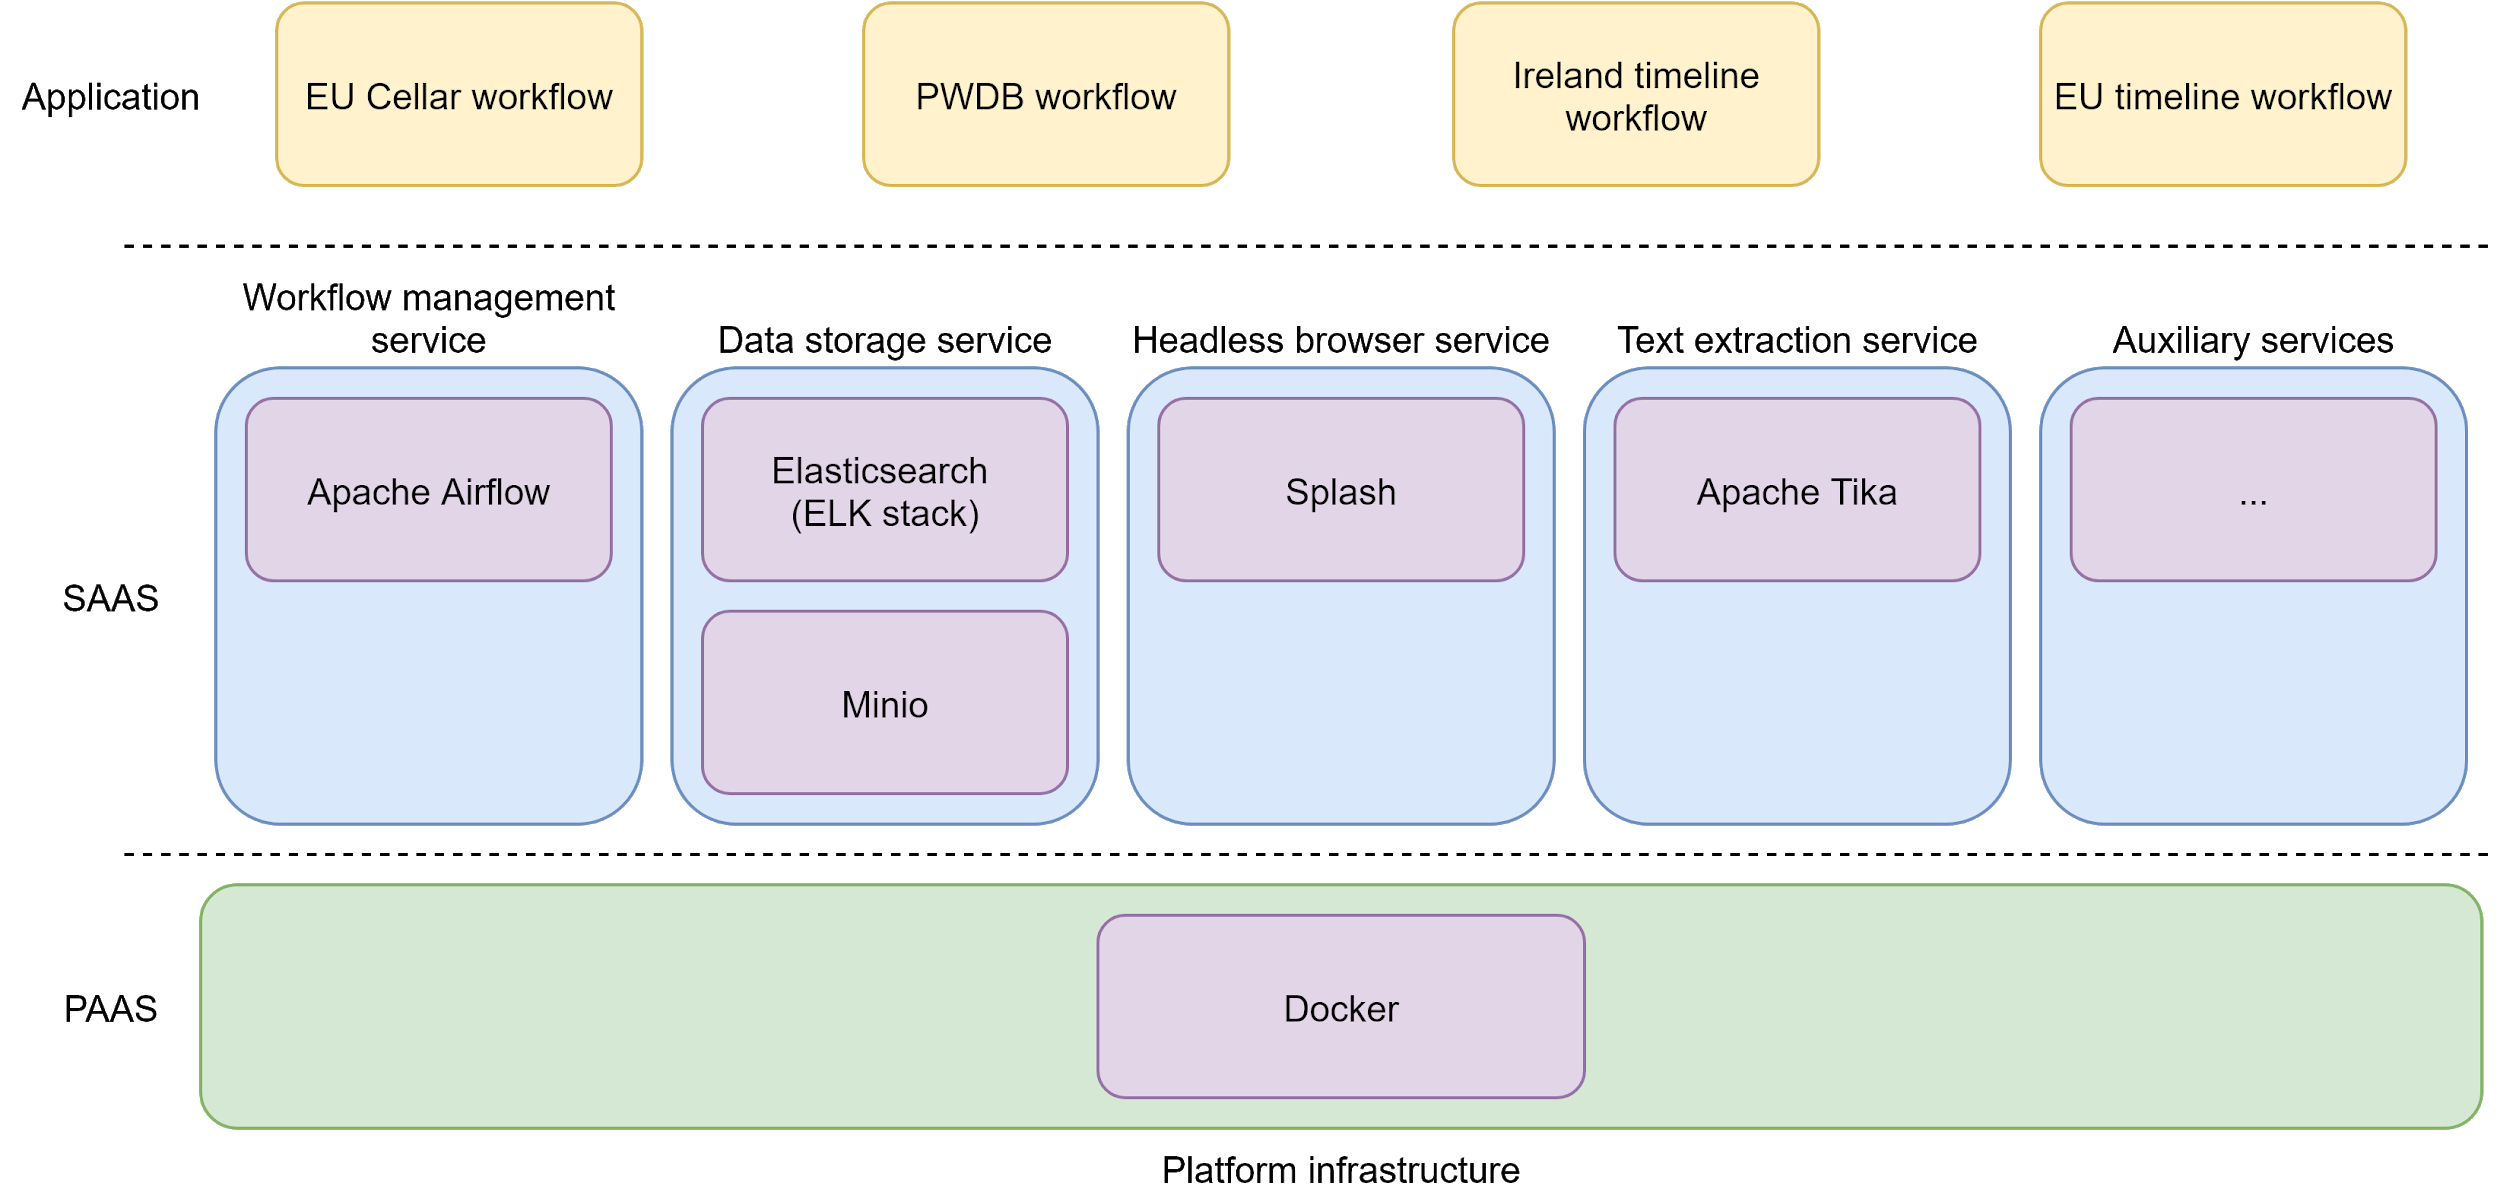
\includegraphics[width=\textwidth]{images/image3.png}
		\caption{Technology stack overview}
		\label{fig:Technology_stack_overview}
	\end{Center}
\end{figure}
%%%%%%%%%%%%%%%%%%%% Figure/Image No: 3 Ends here %%%%%%%%%%%%%%%%%%%%

The diagram in Figure \ref{fig:Technology_stack_overview} is split into three layers: \textit{Platform as a Service (PaaS) layer, Software as a Service (SaaS) layer, and Application layer}. 

\enlargethispage{2em}

At the bottom of the diagram is depicted the infrastructure layer. We have decided to operate based on a platform infrastructure because it abstracts away from the traditional physical servers and allows a deployment virtually in any environment: physical server, virtual machine, cloud. The chosen PaaS technology is Docker\footnote{Docker is a set of platform as a service (PaaS) products that use OS-level virtualization to deliver software in packages called containers. } for its popularity and relative simplicity over alternatives such as Kubernetes\footnote{Kubernetes is an open-source system for automating deployment, scaling, and management of containerized applications.}. 

In the middle of the diagram are depicted five larger blue round-cornered rectangles five. They represent classes of services we're employing in this project. These services are: \textit{workflow management system, data} \textit{storage service, headless browser service, text processing service, }and auxiliary services. We will explain below how each is used after we address the application layer workflow structure. 

In the top part of the diagram is depicted the application layer which contains four workflows, one for each dataset: \textit{EU Cellar workflow}, \textit{EU timeline workflow}, \textit{PWDB workflow}, and \textit{Ireland timeline workflow}. These workflows have a prototypical extract, transform, toad (ETL) structure\footnote{ In computing, extract, transform, load (ETL) is the general procedure of copying data from one or more sources into a destination system which represents the data differently from the source(s) or in a different context than the source(s). The ETL process became a popular concept in the 1970s and is often used in data warehousing. }. The generic ETL process implemented in our workflows is addressed in the next section.

\section{Workflow structure: how it works? }
\label{sec:how-it-works}

This section addresses the general structure of dataset creation workflow. Because it is a simple sequence of tasks, without any major bifurcations we call them pipelines as well. The prototypical pipeline we implement is depicted in Figure \ref{fig:Generic_ETL_process_for_dataset_creation} and can be conceptualised as a sequence of four steps: 

\begin{itemize}
	\item data\textit{ extraction} from the source and storage in the temporary object storage
	\item data \textit{structure transformation} in the temporary storage
	\item data \textit{content transformation} in the temporary storage

	\item final data\textit{ loading} into the document repository
\end{itemize}

The sources of data we employ in this project are: 

\begin{itemize}
	\item Cellar SPARQL endpoint\footnote{ \href{http://publications.europa.eu/webapi/rdf/sparql}{Cellar SPARQL endpoint} } where the EU legal documents are stored and disseminated. 
	\item Eurofound website\footnote{ \href{https://www.eurofound.europa.eu/data/covid-19-eu-policywatch}{Eurofound PWDB download page} } where the PWDB is published.
	\item EU action timeline page

	\item Ireland government press corner page
\end{itemize}

\begin{Center}
%%%%%%%%%%%%%%%%%%%% Figure/Image No: 4 starts here %%%%%%%%%%%%%%%%%%%%
\begin{figure}[h]
	\begin{Center}
		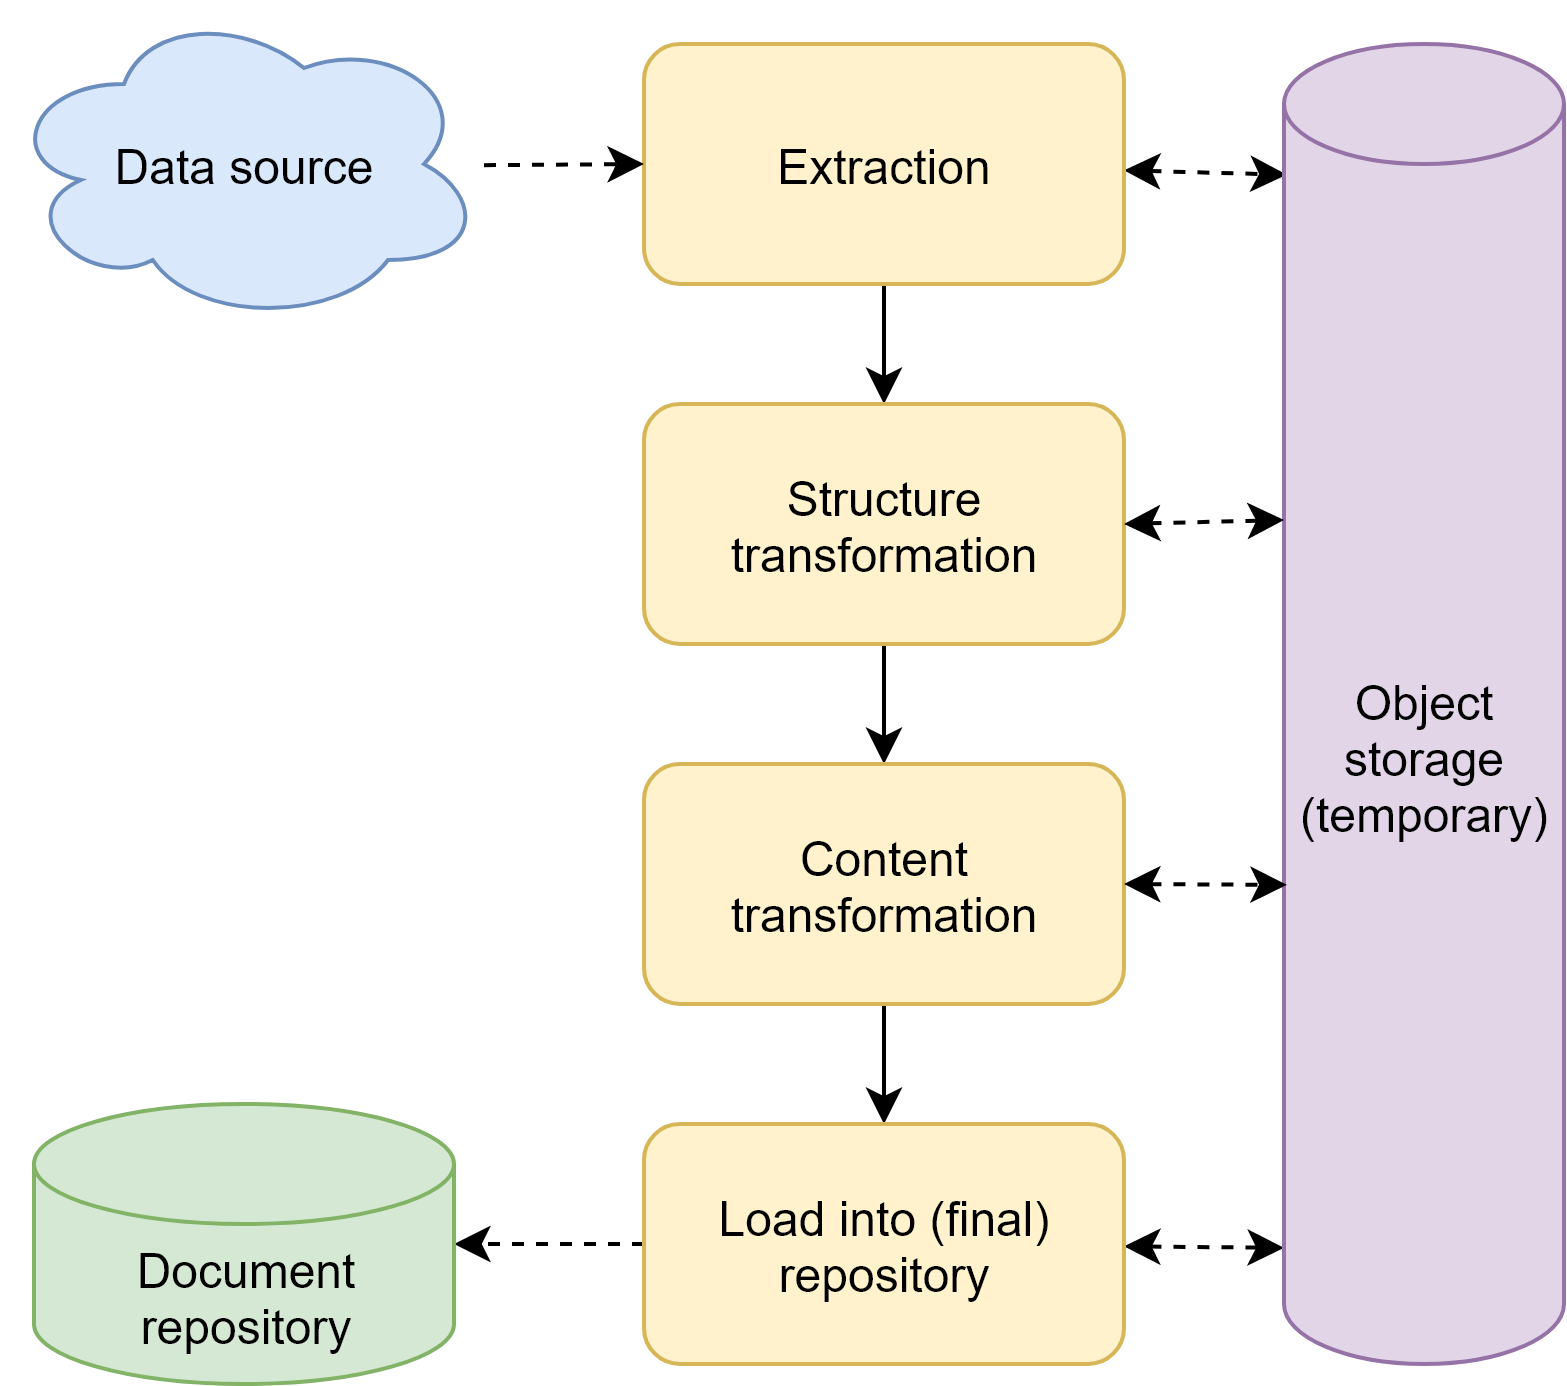
\includegraphics[width=4.24in,height=3.75in]{images/image5.png}
		\caption{Generic ETL process for dataset creation}
		\label{fig:Generic_ETL_process_for_dataset_creation}
	\end{Center}
\end{figure}
%%%%%%%%%%%%%%%%%%%% Figure/Image No: 4 Ends here %%%%%%%%%%%%%%%%%%%%
\end{Center}

\subsection{Extraction}

The process starts with \textit{extracting} the necessary data from the source and storing it in temporary object storage at our premises, making it available for further processing. Doing so enables us to process arbitrarily large amounts of data compared to the alternative of keeping the extracted data in memory, which is relatively limited on the traditional systems. 

Besides simple HTTP requests\footnote{ \href{https://en.wikipedia.org/wiki/Hypertext_Transfer_Protocol}{HTTP} is an application layer protocol for distributed, collaborative, hypermedia information systems. HTTP is the foundation of data communication for the World Wide Web. }, the extraction operations important to mention are the \textit{SPARQL querying} and \textit{Website crawling}. 

SPARQL\footnote{ \href{https://www.w3.org/TR/sparql11-query/}{SPARQL Protocol and RDF Query Language} } is a semantic query language able to retrieve and manipulate data stored in RDF\footnote{ \href{https://www.w3.org/TR/rdf11-concepts/}{Resource Description Framework}  } format. We query Cellar, the European semantic repository, for legal documents annotated with COVID-19 tag or related EuroVoc concepts. 

A \textit{Web crawler\footnote{ \href{https://en.wikipedia.org/wiki/Web_crawler}{Web crawler} }} sometimes called a \textit{spider} and often shortened to \textit{crawler}, is an Internet bot that systematically browses the World Wide Web, typically operated by search engines for the purpose of Web indexing. We developed two crawlers, using Scrapy library\footnote{ \href{https://en.wikipedia.org/wiki/Scrapy}{Scrapy}, a fast high-level web crawling $\&$  scraping framework for Python. }, first to fetch information from the EU action timeline website, and the second one from the Ireland government press corner. Scrapy is a free and open-source web-crawling framework written in Python. Originally designed for web scraping, it can also be used to extract data using APIs or as a general-purpose web crawler.

In the scraping process, often simple HTTP requests are not sufficient for performing full content extraction. Execution of custom JavaScript code is necessary to complete the page loading. For this purpose, headless browser services are typically implemented. They simulate the behaviour of a web browser but without having the interface of one. We employ Splash\footnote{ \href{https://splash.readthedocs.io/en/stable/}{Splash} javascript rendering service } to act as a headless browser. Splash is a javascript rendering service with an HTTP API. It's a lightweight browser with an HTTP API, implemented in Python 3. In combination with Scrapy, Splash allows us to crawl the two web sources successfully. 

One other aspect essential to mention here is that we employ an object storage service called Minio\footnote{ \href{https://min.io/}{MinIO} is an open source implementation of the Amazon S3 storage system.  } for the temporary persistence of the extracted data. MinIO is an Amazon S3 compatible server-side software storage stack. It can handle unstructured data such as photos, videos, log files, backups, and container images with the maximum supported object size of 5TB.

One may argue that such an object storage system is unnecessary as the created datasets, so far, are relatively small in size and can easily fit into the memory of most systems. However, this infrastructure, we intend to extend and use for the processing of much larger datasets exceeding the memory limits. That situation will inevitably invite the usage of such a persistence system, which we foresee and introduce upfront.

\subsection{Structure transformation}

Next, we proceed with \textit{structural transformation} to \textit{normalise} the data representation, simplify it, and increase its usability yet maintaining the maximally helpful structure. For convenience, we aim to represent the data in JSON format following the following system: \textit{an array of objects with a unique identifier and an arbitrary number of atomically typed attributes}. The structure is depicted using an example of prototypical JSON objects in Figure \ref{fig:Example_of_prototypical_JSON_objects_on_the_left_valid_and_on_the_right_an_invalid_structure}. 

The attributes may be of any atomic type, such as numbers, strings, dates, etc. or arrays of atomic types (as depicted on the left side of Figure \ref{fig:Example_of_prototypical_JSON_objects_on_the_left_valid_and_on_the_right_an_invalid_structure}), but not objects or arrays of objects (as depicted on the right side of Figure \ref{fig:Example_of_prototypical_JSON_objects_on_the_left_valid_and_on_the_right_an_invalid_structure}). We discourage, with some exceptions, using the embedded object structures. The reason for it is that the embedded objects are no longer easily accessible in the data frame structures (using the numpy\footnote{ Numpy is a library for the Python programming language, adding support for large, multi-dimensional arrays and matrices, along with a large collection of high-level mathematical functions to operate on these arrays. } or Pandas\footnote{ Pandas is a software library written for the Python programming language for data manipulation and analysis. } libraries). The data frames or other tabular representations are the de facto representation for machine learning and data science exercises, which we plan to undertake in the current project.

\begin{Center}
%%%%%%%%%%%%%%%%%%%% Figure/Image No: 5 starts here %%%%%%%%%%%%%%%%%%%%
\begin{figure}[H]
	\begin{Center}
		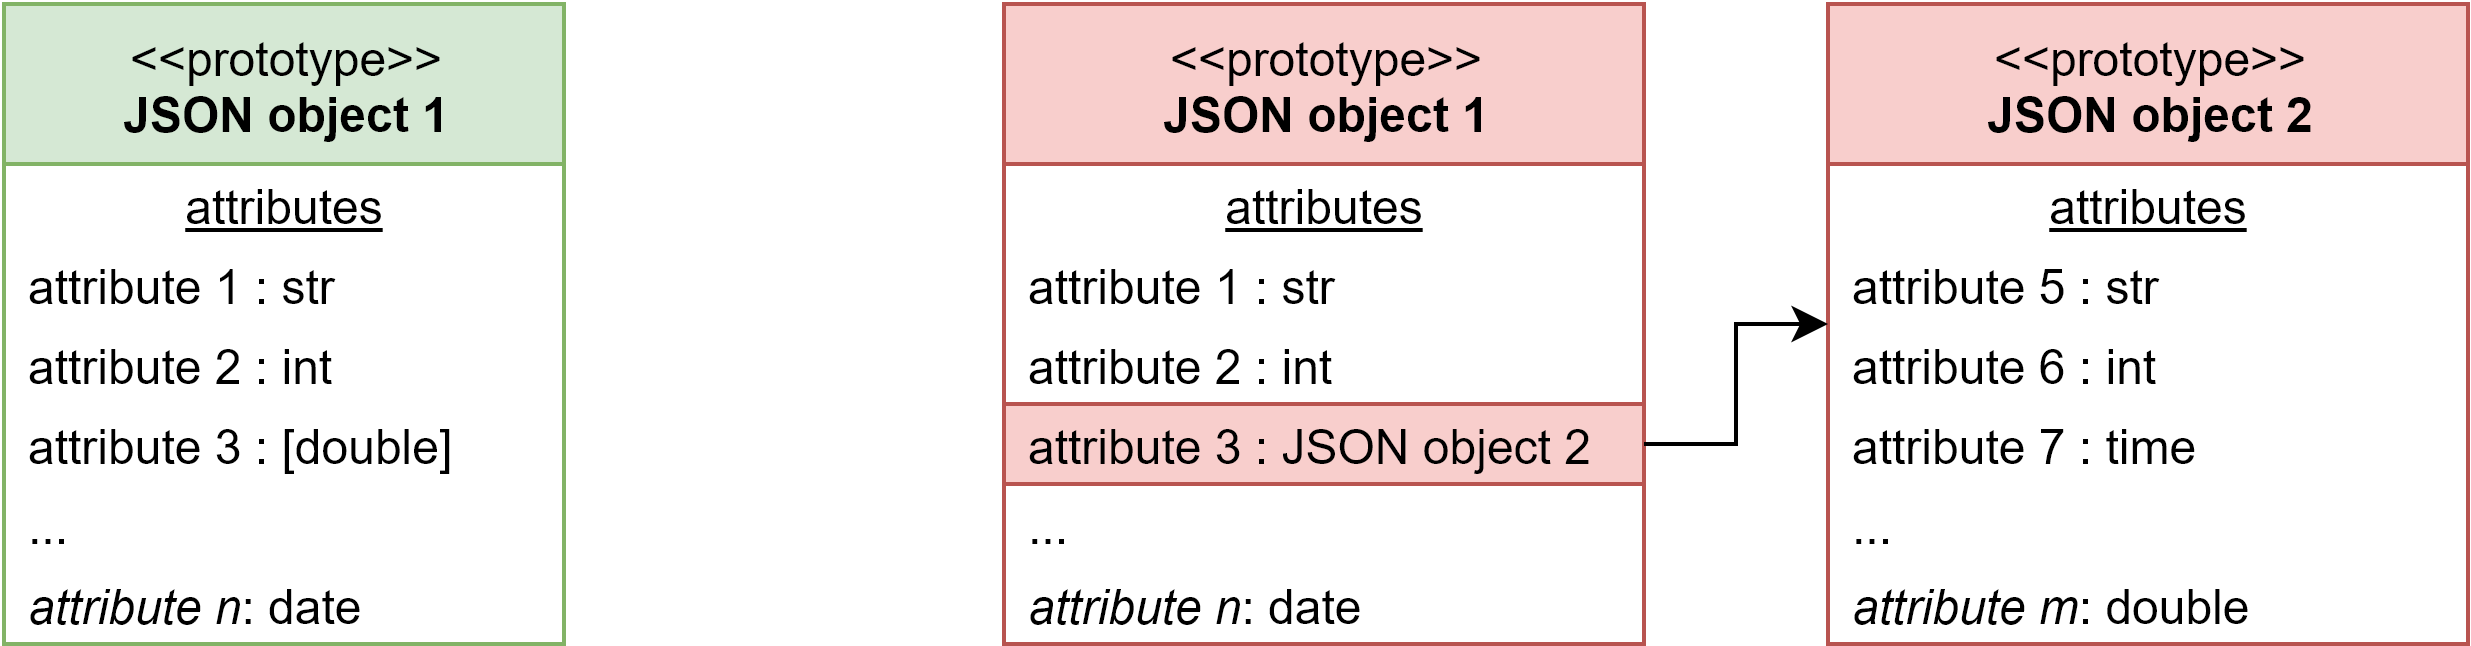
\includegraphics[width=\textwidth]{images/image1.png}
		\caption{Example of prototypical JSON objects, on the left valid and on the right an invalid structure}
		\label{fig:Example_of_prototypical_JSON_objects_on_the_left_valid_and_on_the_right_an_invalid_structure}
	\end{Center}
\end{figure}
%%%%%%%%%%%%%%%%%%%% Figure/Image No: 5 Ends here %%%%%%%%%%%%%%%%%%%%
\end{Center}

For consistency and programming language neutrality, we chose to employ JQ JSON processor\footnote{ ./jq is a lightweight and flexible command-line JSON processor }. The transformation rules are written in JQ language and tailor-made for each data source. As our implementation is entirely written in Python, we use the python library to execute these JQ transformation rules.

\subsection{Content transformation}

fter the data structure is \textit{normalised,} the content transformation generally consists of \textit{text extraction}, \textit{enrichment}, \textit{restructuring, aggregation,} and other operations. 

One peculiarity of this stage is that the initially extracted data contains links and references to other externally available resources. We have carefully analysed and decided to fetch the resources behind selected sets of links. Each dataset includes attributes with such links, which we access and inject the content as an additional attribute. This is what we call content enrichment: injecting extracted content into the dataset. 

The fetched content is in the majority of cases of unpredictable serialisation format, structure and language. Therefore, before it is injected into the dataset, we first \textit{reduce} it to simple texts, which is the foremost valuable data representation for the NLP tasks.

For the \textit{text extraction task,} we decided to use the Apache Tika\footnote{ Apache Tika is a toolkit that detects and extracts metadata and text from over a thousand different file types (such as HTML, PPT, XLS, and PDF). } toolkit. Apache Tika is a library that is used for document type detection and content extraction from various file formats. Internally, Tika uses existing different document parsers and document type detection techniques to detect and extract data. Tika is widely used while developing search engines to index the text contents of digital documents.

Some categorical data attributes are provided as items from a flat fine-grained classification. For practical reasons, it is helpful to reduce the classification scheme. This \textit{restructuring is possible to undergo} by \textit{aggregating} fine-grained categories in terms of more coarse-grained ones. One such example is the target group attribute from PWDB. There are 42 distinct values, which can be roughly categorised as belonging to three more prominent categories. We proceed to inject such aggregations as additional attributes to leverage exploratory data analysis in future stages of the project. 

\subsection{Loading into the repository}

After the structure and content of the data have been restructured, the data is loaded into a repository where it is indexed and made available for querying and full-text search. Because the current datasets are designed for NLP tasks, the full-text search capability is critical. It plays an essential role in the exploratory data analysis and possible data segmentation or partitioning for machine learning experiments. 

For this purpose, we decided to use the Elasticsearch search engine\footnote{ Elasticsearch is a search engine based on the Lucene library. It provides a distributed, multitenant-capable full-text search engine with an HTTP web interface and schema-free JSON documents. } to act as the document repository. It is a real-time distributed and analytic engine that helps in performing various kinds of search mechanisms. It can achieve fast search responses because, instead of searching the text directly, it searches an index instead. Additionally, it supports full-text search, which is completely based on documents instead of tables or schemas that are easier to write queries and manipulate with this textual data. Some of the strongest points of elastic search are:

\begin{itemize}
	\item Performing and combining various kinds of searches irrespective of their data type.
	\item Querying can retrieve data in any form required.
	\item Analyzing billions of records in a few seconds.
	\item Aggregating data enables us to explore trends and patterns.
\end{itemize}

When the datasets are loaded into the Elasticsearch, they are easily explorable using Kibana\footnote{ Kibana is a data visualization dashboard software for Elasticsearch. It provides visualization capabilities on top of the content indexed on an Elasticsearch cluster. } discovery and dashboard functionality. Kibana offers histograms, line graphs, pie charts, sunbursts, geospatial map displays, and other standard visualisation options and the opportunity to create unique visualisations. It also makes it possible for users to spot and analyse relationships or anomalies in the data. Furthermore, the datasets are available for use in machine learning experiments and exploratory data analysis. 

\section{Workflow management system}

The workflows mentioned above are deployed and executed in a workflow management system. Doing so drives automation and leads to increased control, transparency and trust in the execution results. It allows for close monitoring of each step, schedule executions, increased connectivity, eliminates manual tasks, reduces errors, retries on failure, and investigates causes and visualises the workflow, control panel, and other benefits. 

We have chosen Apache Airflow system\footnote{ Apache Airflow is an open-source workflow management platform. It started at Airbnb in October 2014 as a solution to manage the company's increasingly complex workflows. } due to its architectural choices, maturity, rich set of features, strong community, rich set of integrations and plugins, and because a system implemented in Python fits well our Python predominant technical stack. 

Airflow is a platform to programmatically author, schedule and monitor workflows. It is written in Python, and workflows are created via Python scripts, called DAGs (Directed Acyclic Graphs). An example DAG structure is depicted in Figure \ref{fig:Example_of_a_DAG_structure}. 

Airflow is designed under the principle of ``\textit{configuration as code}'' . While other ``\textit{configuration as code}''  workflow platforms exist using markup languages like XML, using Python allows developers to import libraries and classes to help them create their workflows.

\begin{Center}
%%%%%%%%%%%%%%%%%%%% Figure/Image No: 6 starts here %%%%%%%%%%%%%%%%%%%%
\begin{figure}[H]
	\begin{Center}
		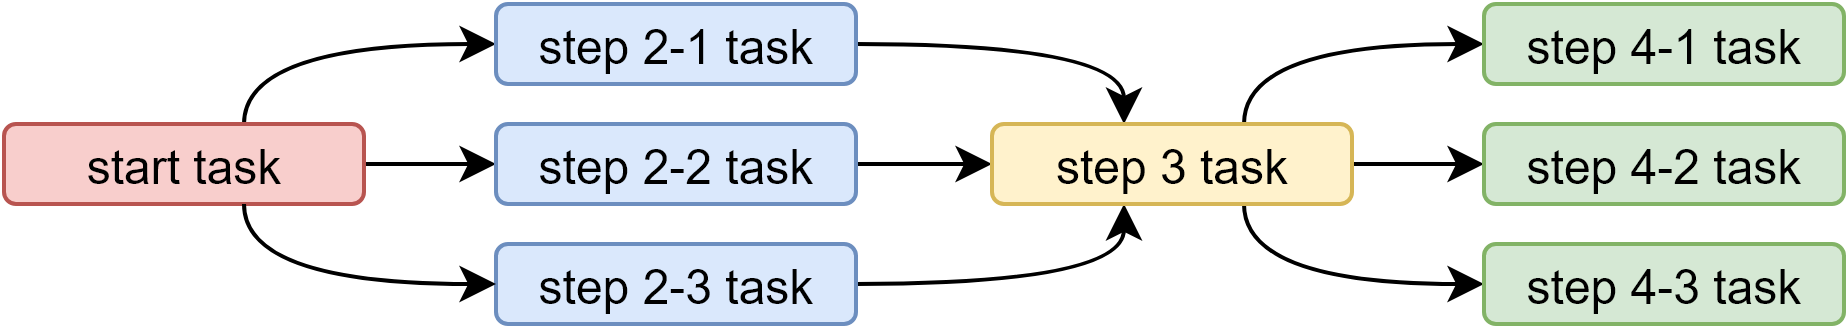
\includegraphics[width=\textwidth]{images/image2.png}
		\caption{Example of a DAG structure}
		\label{fig:Example_of_a_DAG_structure}
	\end{Center}
\end{figure}
%%%%%%%%%%%%%%%%%%%% Figure/Image No: 6 Ends here %%%%%%%%%%%%%%%%%%%%
\end{Center}

Airflow uses directed acyclic graphs (DAGs\footnote{ A DAG is a collection of all the tasks you want to run, organized in a way that reflects their relationships and dependencies. }) to manage workflow orchestration. Tasks and dependencies are defined in Python and then Airflow manages the scheduling and execution. DAGs can be run either on a defined schedule (e.g. hourly or daily) or based on external event triggers.

DAG, or directed acyclic graphs, are a collection of all of the tasks, units of work in the pipeline. The tasks are organised by their relationships and dependencies between each other. A directed acyclic graph implies that your pipeline can only move forwards, not backwards. A task can retry, but a task can't be rerun after it has completed and another task downstream has begun.

Using Airflow enables us to organise our pipelines as DAGs, develop project-specific functionality and incorporate it seamlessly into the workflow architecture to deploy and execute in a robust environment easily.

\section{Limitations and future work}

In the process of developing the current dataset, a number of limitations were set to the scope of this project. This section covers a non-exhaustive list of these limitations and how they may be addressed in future work.

Currently, the dataset is limited to the English language. In future work, the dataset can be expanded to cover member state measures individually. Doing so will inevitably lead to creating a multilingual dataset containing texts in 24 official European languages. This is mainly because the authorities publish the measures in that country's official language(s).

Using different text registers implies a disparate treatment of texts in the analysis and processing pipelines. Developing a mechanism to summarise a document to extract measure description from it, as, for example, would be necessary for large legal texts, would be of tremendous benefit for harmonisation of the dataset content across various sources. Addressing this in future work will yield an advantage for the exploratory data analysis and other machine learning exercises.

Another axis of homogenisation would be to bring all the texts to a common language, such as English, for example. To do so would necessitate translation services, which at the moment were not used. Having done so will decrease the linguistic fragmentation of the dataset, leading to a larger homogeneous corpus, which increases the statistical significance of the results produced based on this dataset.

\enlargethispage{2em}


%\chapter{Architecture building blocks}
\label{sec:building-blocks}

	This chapter provides some foundations about the notations, definitions and the general approach adopted here to model the enterprise architecture.

	\section{Methodology}
	
	In this document we take an enterprise architecture perspective and aim to provide several architecture views (see Section \ref{sec:views}) which are necessary and sufficient to describe the asset lifecycle process. 
	
	In developing this architecture, we are in part using the TOGAF \citep{togaf9.2} methodology, which is, in fact, a framework for enterprise architecture that provides an approach for designing, planning, implementing and governing an enterprise information technology architecture. Although we do not follow this framework extensively, relevant parts of it were applied to the goals of this architecture.
		
	For representing the architecture models, ArchiMate language \citep{archimate3.1} is adopted. It is an open and independent enterprise architecture modelling language to support the description, analysis and visualisation of architecture within and across business domains in a clear and unambiguous way.

	Based on the initial requirements specifications document \citep{lam-requirements-2020} and a series of interviews conducted with the LAM team, the structure of the project stakeholders motivations was established. It is presented in Section \ref{sec:motivation-architecture}.
		 
	The business and application layers of this architecture, are a gradual fleshing out of the use cases presented in the project preliminary requirements \citep{lam-preliminary-requirements-2019}, the functional requirements in the requirements specifications document \citep{lam-requirements-2020} and the architecture for managing and publishing semantic assets \citep{costetchi2020d} adopted by the A2 unit.
	 
	The ArchiMate diagrams corresponding to each architecture layer were modelled and designed using Enterprise Architect Tool \citep{ea}. Finally this report was written covering the overall architecture. 
	
	\section{Architecture views}
	\label{sec:views}
	
% 	The next sections of this document we will organise the architecture diagrams based on specific views. An architecture view is a representation of a system from the perspective of a related set of concerns. 
	
	Architecture views are an ideal mechanism to purposefully convey information about architecture areas. In general, a view is defined as a part of an Architecture Description that addresses a set of related concerns and is tailored for specific stakeholders. A view is specified by means of an architecture viewpoint, which prescribes the concepts, models, analysis techniques, and visualisations that are provided by the view. Simply put, a view is what you see, and a viewpoint is where you are looking from \citep{archimate3.1}.
	
	An architecture view expresses the architecture of the system of interest in accordance with an architecture viewpoint (or simply ``viewpoint''). There are two aspects to a viewpoint: the concerns it frames for the stakeholders and the conventions it establishes on views \citep{archimate3.1}.

	Viewpoints are designed for the purpose of communicating certain aspects and layers of an architecture. In this document we address \textit{the motivation view} (Section \ref{sec:motivation-architecture}), \textit{the business view} (Section \ref{sec:business-architecture}), and \textit{the application view} (Section \ref{sec:application-architecture}).
	
	Instead of describing what each of these views represents in this section, we decided to provide such a description in the beginning of each of the subsequent sections. This way, we aim to ease reading the section by providing the reader a fresh introduction into the structure of a prototypical layer architecture before the actual architecture is described.
	
	\section{ArchiMate elements}
	
    This section presents the ArchiMate elements, in terms of their definition and the graphical notation, which we employ in each of the architecture views. 


\begin{longtable}[c]{@{}lll@{}}
	\caption{Overview of the relevant motivation elements \citep{archimate3.1}}
	\label{tab:motivation}\\
	\toprule
	\textbf{Element} & \textbf{Definition} & \textbf{Notation} \\* \midrule
	\endfirsthead
	%
	\multicolumn{3}{c}%
	{{\itshape Table \thetable\ continued from previous page}} \\
	\endhead
	%
	\bottomrule
	\endfoot
	%
	\endlastfoot
	%
			Stakeholder & \parbox{.56\linewidth}{Represents the role of an individual, team, or organisation (or classes thereof) that represents their interests in the effects of the architecture.} &     \cincludegraphics[height=2.5\normalbaselineskip]{images/views/elements/stakeholder}   \\

			Driver & \parbox{.56\linewidth}{Represents an external or internal condition that motivates an organisation to define its goals and implement the changes necessary to achieve them.} & \cincludegraphics[height=2.5\normalbaselineskip]{images/views/elements/driver}  \\
			
			Assessment & \parbox{.56\linewidth}{Represents the result of an analysis of the state of affairs of the enterprise with respect to some driver.} & \cincludegraphics[height=2.5\normalbaselineskip]{images/views/elements/assesment}   \\
			
			Goal & \parbox{.56\linewidth}{Represents a high-level statement of intent, direction, or desired end state for an organisation and its stakeholders.} & \cincludegraphics[height=2.5\normalbaselineskip]{images/views/elements/goal}  \\
			\bottomrule

	\end{longtable}
	
	% Please add the following required packages to your document preamble:
	% \usepackage{booktabs}
	% \usepackage{longtable}
	% Note: It may be necessary to compile the document several times to get a multi-page table to line up properly
	\begin{longtable}[c]{@{}lll@{}}
		\caption{Overview of the relevant business layer elements \citep{archimate3.1}}
		\label{tab:business}\\
		\toprule
		\textbf{Element} & \textbf{Definition} & \textbf{Notation} \\* \midrule
		\endfirsthead
		%
		\multicolumn{3}{c}%
		{{\itshape Table \thetable\ continued from previous page}} \\
		\endhead
		%
		\bottomrule
		\endfoot
		%
		\endlastfoot
		%
			Business actor & \parbox{.5\linewidth}{Represents a business entity that is capable of performing behaviour.} & \cincludegraphics[height=1.82\normalbaselineskip]{images/views/business-elements/actor} \\
			Business role & \parbox{.5\linewidth}{Represents the responsibility for performing specific behaviour, to which an actor can be assigned, or the part an actor plays in a particular action or event.} & \cincludegraphics[height=1.82\normalbaselineskip]{images/views/business-elements/role} \\
			\parbox{.1\linewidth}{Business collaboration} & \parbox{.5\linewidth}{Represents an aggregate of two or more business internal active structure elements that work together to perform collective behaviour.} & \cincludegraphics[height=1.82\normalbaselineskip]{images/views/business-elements/collaboration} \\
			Business interface & \parbox{.5\linewidth}{Represents a point of access where a business service is made available to the environment.} & \cincludegraphics[height=1.82\normalbaselineskip]{images/views/business-elements/interface} \\
			Business process & \parbox{.5\linewidth}{Represents a sequence of business behaviours that achieves a specific result such as a defined set of products or business services.} & \cincludegraphics[height=1.82\normalbaselineskip]{images/views/business-elements/process} \\
			Business function & \parbox{.5\linewidth}{Represents a collection of business behaviour based on a chosen set of criteria (typically required business resources and/or competencies), closely aligned to an organisation, but not necessarily explicitly governed by the organisation.} & \cincludegraphics[height=1.82\normalbaselineskip]{images/views/business-elements/function} \\
			Business event & \parbox{.5\linewidth}{Represents an organisational state change.} & \cincludegraphics[height=1.82\normalbaselineskip]{images/views/business-elements/event} \\
			Business service & \parbox{.5\linewidth}{Represents explicitly defined behaviour that a business role, business actor, or business collaboration exposes to its environment.} & \cincludegraphics[height=1.82\normalbaselineskip]{images/views/business-elements/service} \\
			Business object & \parbox{.5\linewidth}{Represents a concept used within a particular business domain.} & \cincludegraphics[height=1.82\normalbaselineskip]{images/views/business-elements/object} \\
			Representation & \parbox{.5\linewidth}{Represents a perceptible form of the information carried by a business object.} & \cincludegraphics[height=1.82\normalbaselineskip]{images/views/business-elements/representation} \\ \bottomrule
		
	\end{longtable}

	% Please add the following required packages to your document preamble:
	% \usepackage{booktabs}
	% \usepackage{longtable}
	% Note: It may be necessary to compile the document several times to get a multi-page table to line up properly
	\begin{longtable}[c]{@{}lll@{}}
		\caption{Overview of the relevant application layer elements \citep{archimate3.1}}
		\label{tab:application}\\
		\toprule
		\textbf{Element} & \textbf{Definition} & \textbf{Notation} \\* \midrule
		\endfirsthead
		%
		\multicolumn{3}{c}%
		{{\itshape Table \thetable\ continued from previous page}} \\
		\endhead
		%
		\bottomrule
		\endfoot
		%
		\endlastfoot
		%
			\parbox{.1\linewidth}{Application component} & \parbox{.5\linewidth}{Represents an encapsulation of application functionality aligned to implementation structure, which is modular and replaceable.} & \cincludegraphics[height=1.82\normalbaselineskip]{images/views/application-elements/component} \\
			\parbox{.1\linewidth}{Application interface} & \parbox{.5\linewidth}{Represents a point of access where application services are made available to a user, another application component, or a node.} & \cincludegraphics[height=1.82\normalbaselineskip]{images/views/application-elements/interface} \\
			\parbox{.1\linewidth}{Application function} & \parbox{.5\linewidth}{Represents automated behaviour that can be performed by an application component.} & \cincludegraphics[height=1.82\normalbaselineskip]{images/views/application-elements/function} \\
			\parbox{.1\linewidth}{Application process} & \parbox{.5\linewidth}{Represents a sequence of application behaviours that achieves a specific result.} & \cincludegraphics[height=1.82\normalbaselineskip]{images/views/application-elements/process} \\
			\parbox{.1\linewidth}{Application event} & \parbox{.5\linewidth}{Represents an application state change.} & \cincludegraphics[height=1.82\normalbaselineskip]{images/views/application-elements/event} \\
			\parbox{.1\linewidth}{Application service} & \parbox{.5\linewidth}{Represents an explicitly defined exposed application behaviour.} & \cincludegraphics[height=1.82\normalbaselineskip]{images/views/application-elements/service} \\
			\parbox{.15\linewidth}{Data object} & \parbox{.5\linewidth}{Represents data structured for automated processing.} & \cincludegraphics[height=1.82\normalbaselineskip]{images/views/application-elements/object} \\ \bottomrule		
		
	\end{longtable}

	% Please add the following required packages to your document preamble:
	% \usepackage{booktabs}
	% \usepackage{longtable}
	% Note: It may be necessary to compile the document several times to get a multi-page table to line up properly
	\begin{longtable}[c]{@{}lll@{}}
		\caption{Overview of the relevant technology layer elements \citep{archimate3.1}}
		\label{tab:technology}\\
		\toprule
		\textbf{Element} & \textbf{Definition} & \textbf{Notation} \\* \midrule
		\endfirsthead
		%
		\multicolumn{3}{c}%
		{{\itshape Table \thetable\ continued from previous page}} \\
		\endhead
		%
		\bottomrule
		\endfoot
		%
		\endlastfoot
		%
			Node & \parbox{.5\linewidth}{Represents a computational or physical resource that hosts, manipulates, or interacts with other computational or physical resources.} & \cincludegraphics[height=1.82\normalbaselineskip]{images/views/technology-elements/node} \\
			Device & \parbox{.5\linewidth}{Represents a physical IT resource upon which system software and artefacts may be stored or deployed for execution.} & \cincludegraphics[height=1.82\normalbaselineskip]{images/views/technology-elements/device} \\
			\parbox{.15\linewidth}{System software} & \parbox{.5\linewidth}{Represents software that provides or contributes to an environment for storing, executing, and using software or data deployed within it.} & \cincludegraphics[height=1.82\normalbaselineskip]{images/views/technology-elements/software} \\
			\parbox{.15\linewidth}{Technology interface} & \parbox{.5\linewidth}{Represents a point of access where technology services offered by a node can be accessed.} & \cincludegraphics[height=1.82\normalbaselineskip]{images/views/technology-elements/interface} \\
			\parbox{.18\linewidth}{Communication network} & \parbox{.5\linewidth}{Represents a set of structures that connects nodes for transmission, routing, and reception of data.} & \cincludegraphics[height=1.82\normalbaselineskip]{images/views/technology-elements/network} \\
			\parbox{.15\linewidth}{Technology service} & \parbox{.5\linewidth}{Represents an explicitly defined exposed technology behaviour.} & \cincludegraphics[height=1.82\normalbaselineskip]{images/views/technology-elements/service} \\
			Artefact & \parbox{.5\linewidth}{Represents a piece of data that is used or produced in a software development process, or by deployment and operation of an IT system.} & \cincludegraphics[height=1.82\normalbaselineskip]{images/views/technology-elements/artifact} \\ \bottomrule
		
	\end{longtable}



	\begin{longtable}[c]{@{}lll@{}}
	\caption{Overview of the ArchiMate relationships \cite{archimate3.1}}
	\label{tab:relations}\\
	\toprule	
	\textbf{Element} & \textbf{Definition} & \textbf{Notation} \\* \midrule
	\endfirsthead
	%
	\multicolumn{3}{c}%
	{{\itshape Table \thetable\ continued from previous page}} \\
	\endhead
	%
	\bottomrule
	\endfoot
	%
	\endlastfoot
	%
			\multicolumn{2}{c}{\textbf{Structural Relationships}} & \multicolumn{1}{l}{\textbf{}} \\ 
			Composition & \parbox{.56\linewidth}{Represents that an element consists of one or more other concepts.} & \cincludegraphics[width=4\normalbaselineskip]{images/views/relations/composition} \\
			
			Aggregation & \parbox{.56\linewidth}{Represents that an element combines one or more other concepts.} & \cincludegraphics[width=4\normalbaselineskip]{images/views/relations/aggregation} \\
			Assignment & \parbox{.56\linewidth}{Represents the allocation of responsibility, performance of behaviour, storage, or execution.} & \cincludegraphics[width=3.5\normalbaselineskip]{images/views/relations/assignment} \\
			Realisation & \parbox{.56\linewidth}{Represents that an entity plays a critical role in the creation, achievement, sustenance, or operation of a more abstract entity.} & \cincludegraphics[width=3.5\normalbaselineskip]{images/views/relations/realisation} \\
			\multicolumn{2}{c}{\textbf{Dependency Relationships}} & \multicolumn{1}{l}{\textbf{}} \\ 
			Serving & \parbox{.56\linewidth}{Represents that an element provides its functionality to another element.} & \cincludegraphics[width=4\normalbaselineskip]{images/views/relations/serving} \\
			Access & \parbox{.56\linewidth}{Represents the ability of behaviour and active structure elements to observe or act upon passive structure elements.} & \cincludegraphics[width=4\normalbaselineskip]{images/views/relations/access} \\
			Influence & \parbox{.56\linewidth}{Represents that an element affects the implementation or achievement of some motivation element.} & \cincludegraphics[width=4\normalbaselineskip]{images/views/relations/influence} \\
			Association & \parbox{.56\linewidth}{Represents an unspecified relationship, or one that is not represented by another ArchiMate relationship.} & \cincludegraphics[width=4\normalbaselineskip]{images/views/relations/association} \\
			\multicolumn{2}{c}{\textbf{Dynamic Relationships}} & \multicolumn{1}{l}{\textbf{}} \\ \midrule
			Triggering & \parbox{.56\linewidth}{Represents a temporal or causal relationship between elements.} & \cincludegraphics[width=4\normalbaselineskip]{images/views/relations/triggers} \\
			Flow & \parbox{.56\linewidth}{Represents transfer from one element to another.} &  \cincludegraphics[width=4\normalbaselineskip]{images/views/relations/flows}\\
			\multicolumn{2}{c}{\textbf{Other Relationships}} & \multicolumn{1}{l}{\textbf{}} \\ \midrule
			Specialisation & \parbox{.56\linewidth}{Represents that an element is a particular kind of another element.} & \cincludegraphics[width=3.5\normalbaselineskip]{images/views/relations/specialises} \\			
			Junction & \parbox{.56\linewidth}{Used to connect relationships of the same type.} & \cincludegraphics[width=4\normalbaselineskip]{images/views/relations/junction} \\ \bottomrule
	\end{longtable}

	 \section{Service Oriented Architecture (SOA)}
	 \label{sec:soa}
	 
	 This section provides a motivation for adopting the design guidelines and best practices offered by the \textit{Service Oriented Architecture} (SOA) \cite{open2016soa} paradigm. This is especially important for guiding the development and engineering teams away from a monolith tightly coupled software capabilities that are executed on a dedicated server, towards loosely coupled services exposed through REST APIs capable of running as scalable processes in a distributed environment.
	  
	 \textit{Service-oriented architecture} is a style of software design where services are provided to the other components by application components, through a communication protocol over a network. A SOA service is a discrete unit of functionality that can be accessed remotely and acted upon and updated independently. SOA is also intended to be independent of vendors, products and technologies.
	 
	 SOA is believed to help businesses respond more quickly and more cost-effectively to changing market conditions. This style of architecture promotes high component reuse and facilitates interconnection between components. The SOA systems are known to be resilient in the light of changing technologies because the components are loosely coupled and could easily be replaced by alternative implementations exposing with the same interfaces.	SOA could be regarded as an architectural evolution rather than as a revolution. It captures many of the best practices of previous software architectures and it is a practical approach for cloud computing \citep{velte2019cloud}.
	 
	 Service-oriented architecture can be implemented with web services or Micro-services \citep{brandner2004web}. This is done to make the functional building-blocks accessible over standard Internet protocols that are independent of platforms and programming languages. These services can represent either new applications or just wrappers around existing legacy systems to make them network-enabled \citep{channabasavaiah2003migrating}. By following this approach, the application implementation materialises as a suite of micro-services. Where necessary, the micro-services can be implemented as wrappers around existent components and at a later stage the components can be replaced by new implementations. 
%\chapter{Motivation architecture}
\label{sec:motivation-architecture}

	This chapter presents the motivation and goal structure of the LAM team for this project. This motivation structure is also situated in the context of the Publications Office, this way providing a rationale for the initiative for modelling LAM data in the first place. 
		
	This motivation view helps address questions on why a stakeholder demand for certain capabilities is meaningful, model crucial drivers and root causes behind the demand, actual goals and related outcomes, as well as concrete requirements for further development. In short, it answers the crucial questions to WHOM, WHY and WHAT.
	
	We do not aim for an in depth coverage of the motivation architecture here: in the sense that it cannot be considered as a fully fledged decision-making tool for the management. The focus is to account for the context, stakeholders and their drivers and interests.
	
	\section{Prototypical motivation structure}
	\label{sec:how-to-motivation}		
	
	The structure of motivations, in ArchiMate, is organised hierarchically in several layers. For simplicity, we have chosen to use the top four layers: \textit{stakeholders, drivers, assessments and goals}; leaving out the \textit{outcomes}, \textit{principles} and \textit{requirements}. \mbox{Figure \ref{fig:morivation-structure}} depicts the organisation of the motivation architecture. The structure starts at the top with enumerating the stakeholders, who can be individuals, teams or organisations that represent their interests in the effects of \mbox{the architecture \citep{archimate3.1}}. 
	
	\begin{figure}[h]
		\centering
		\includegraphics[width=0.7\textwidth]{images/views/Motivation view.png}
		\caption{The layered motivation structure}
		\label{fig:morivation-structure}
	\end{figure}
	
	\textit{Stakeholders} have associated interests, concerns or \textit{drivers}, which represent internal or external conditions that motivate an organisation to define goals.
	
	\textit{Assessments} represent results of analysis of the state of affairs with respect to a driver. They reveal strengths and weaknesses, opportunities and threats to an area of interest. Assessments are associated with \textit{goals} which represent a high-level statement of intent, plus direction to desired end state for an organisation and its stakeholders \citep{archimate3.1}. 
	
	In the context of the current project the following stakeholders have been identified:
	
	\enlargethispage{1em}
	
	\begin{itemize}
		\item OP legal analysis team (OP.C.2.003)
		\item Different OP services
		\item EU institutions
		\item LAM contractors
		\item Publications Office of the European Union (OP)
	\end{itemize}

	Next we present the motivation structure of spread over several sections addressing each stakeholder in part.
	
	\section{OP legal analysis team}

	The legal analysis team at the OP is the main stakeholder in this project. The main driver of this team is to establish a single point of access for the LAM data that can serve also as the single point of truth for this dataset. 
	
	\begin{figure}[h]
	\centering
	\includegraphics[width=0.67\textwidth]{images/motivation/LAM team motivation.png}
	\caption{Motivation structure of the OP legal analysis team}
	\label{fig:motivation-lam-team}
	\end{figure}
	
	One particular feature that is of special importance is to to also link other various datasets on which LAM relies, such as Common Data Model (CDM) \citep{cdm-francesconi2015ontology, cdm-francesconi2015semantic}, authority tables published at the EU Vocabularies\footnote{\url{https://op.europa.eu/en/web/eu-vocabularies}}, European Legislation Identifier (ELI) and others. The linked LAM information driver is a sub-goal to establishing a single point of access driver, and this is modelled via part-of relationship in \mbox{Figure \ref{fig:motivation-lam-team}}.
	
	In the context of the project these two drivers are hindered by three issues. First, multiple sources of information published in an uncoordinated manner on disparate sources are difficult to access and consume. This is especially the case when the information available at decentralised data sources needs to be used coherently in combination with other data sources.

	Another issue is that the meaning, rules and dependencies of the LAM model are sometimes not known by the stakeholders due to various reasons. One reason is the failure to find this information. Another reason is the informal explanation which may be incomplete, ambiguous or vague leading to multiple interpretations. And this leads to the third issue that the lack of precise formally defined knowledge is further propagated into the domain where LAM is applied and materialises as inconsistencies and mistakes in the data, system implementations, infrastructure configurations, exchange protocols and other aspects of the information systems. 
	
	To overcome these issues the goal of creating a central access point for the LAM data is adopted. This being the main goal of this project (LAM\#2). 	

	\section{Different OP services and EU institutions}
	
	At the Publications Office various internal units and the services they expose operate with legal data and metadata. Having access to the semantic description of the OP legal data is of primary concern for these services collectively. This is schematically depicted in Figure \ref{fig:motivation-op-services}.
	
	\begin{figure}[!th]
		\centering
		\includegraphics[width=0.789\textwidth]{images/motivation/EU institutions and OP services motivation.png}
		\caption{Motivation structure of different OP services}
		\label{fig:motivation-op-services}
	\end{figure}

	Implementation of the single point of access for semantic LAM model can be conceptualised as a sub-driver for the need to access semantic descriptions of OP legal data and metadata, which is represented through an aggregation relation in Figure \ref{fig:motivation-op-services}. Both motivations are hindered by the fact that decentralised access to multiple information sources is slow and inefficient. Moreover, LAM meaning, rules and dependencies are not always known to the interested stakeholders. To overcome these limitations, the current architecture aims at describing how a central dissemination point for LAM can be established. 
	
	The EU institutions, at large, as a collective consumer of legal metadata definitions has the same needs as the OP services. In addition, a notification mechanism is desired to inform the interested players of changes and updates in the LAM data. This need materialises directly as a feature of the system to disseminate LAM data. 
	
	\section{LAM contractors}

	The LAM contractors are a set of special stakeholders as they not only need to consult LAM data for information, but they are the agents that are actively involved in applying the specifications in practice. Often times, they will be those who inform the LAM team about possible issues in the LAM model or request extensions to it in order to accommodate new situations. The main driver for the LAM consultants is the consultancy on LAM and follow-up, depicted in Figure \ref{fig:motivation-lam-contractors}. 
		 	
	\begin{figure}[h]
		\centering
		\includegraphics[width=0.95\textwidth]{images/motivation/LAM Contractors motivation.png}
		\caption{Motivation structure of LAM contractors}
		\label{fig:motivation-lam-contractors}
	\end{figure}

	Traditionally, the LAM model was maintained as a MS Word document that is an unstructured (at least not for the machines) data representation. A direct consequence of this approach is that no automation, validation or consistency checking is possible with such representations. To overcome this limitation an initiative to structure LAM data into a machine readable model was performed at the end of 2019 (referred as LAM\#1 project). LAM\#1 deliverables are available in the \textit{lam4vb3} GitHub repository\footnote{see \url{https://github.com/eu-vocabularies/lam4vb3}}.
		
	Another issue is that, as no machine assistance is possible to implement, the maintenance of these data becomes increasingly more difficult due to highly interlinked nature of the LAM model. This approach does not scale and is inefficient. 
	Moreover the effect is amplified as sometimes the LAM meaning, rules and dependencies are not known by the LAM contractors or even the LAM maintenance team. In order to overcome this limitation, a set of automation functionalities and processes shall be established. This automation is out of current project scope and shall be addressed elsewhere. 
	
	On the left side of Figure \ref{fig:motivation-lam-contractors}, the driver, assessments and goal are repeated from the sections above as they are central to the current project and are, therefore, shared by all of the stakeholders. 

	\section{Publications Office of the European Union}
	
	The Publications Office of the European Union defines drivers at a higher level of abstraction; yet they are very relevant to mention because the current project contributes directly to those interests. Figure \ref{fig:motivation-op} depicts the motivation structure of the OP relevant to the context of the current project. 
	
	OP is interested in the semantic operability both across EU institutions and the intra-institutional information systems. To increase the shared common conceptualisation captured by the data models, they need to carry a certain level of formality, semantics that shall be verifiable for completeness and especially for soundness. Unfortunately not all data is represented in machine readable format and even less is based on semantic models. 
	
	\begin{figure}[!h]
		\centering
		\includegraphics[width=0.859\textwidth]{images/motivation/OP level motivation (higher).png}
		\caption{Motivation structure of the Publications Office of the European Union}
		\label{fig:motivation-op}
	\end{figure}
	
	Another broad OP interest is maintaining and increasing by possible means the data quality. Causes such as lack of or impaired access to knowledge, unfortunately directly leads to inconsistencies and mistakes, which decrease the data quality. In order to overcome these limitations, the creation of a central access point for LAM addressed to a large extent the problem of knowledge shortage is required.
	
	Finally, a driver, which is at the heart of the OP as an institution, is to facilitate discovery of EU legal resources. In the context of the current project, this driver is hindered by the inability to easily find and access LAM meanings, rules and dependencies. Therefore, the dissemination of LAM data shall be done in such a way that the relations to external data sources are presented in an intuitive manner and the links are easy to navigate. Moreover, an inventory of links to the most used resources shall be disseminated with the LAM data. 
	
%\chapter{Business architecture}
\label{sec:business-architecture}
	
	This chapter addresses the business architecture of the initiative to model LAM data. The aim is to describe the internal processes, events and roles answering questions concerning WHO shall do WHAT and WHEN.
	
	This chapter first presents the decontextualised architecture specific to LAM modelling initiative and then proceeds to place the management of the LAM asset in the context of a lifecycle model.
	
	However, the description starts by explaining how a prototypical business architecture is structured and that will serve as a framework to better understand the diagrams in this chapter.
	
	\section{Prototypical business structure}
	
	Following the metaphor of layers presented in the motivation view (see Section \ref{sec:how-to-motivation}), the organisation of business structure is also explained in terms of layers. Figure \ref{fig:business-structure-protopypical} depicts three layers with the most important elements of the business structure. 
	
	\begin{figure}[h]
		\centering
		\includegraphics[width=0.78\textwidth]{images/views/Business view.png}
		\caption{The prototypical business structure view}
		\label{fig:business-structure-protopypical}
	\end{figure} 
	
	The topmost layer accounts for the external players or \textit{actors}, which represent a business entity that is capable of performing behaviour and \textit{roles}, which represent skills and responsibilities for performing specific behaviours, and to which an actor can be assigned \citep{archimate3.1}. 
	
	The middle layer represents the \textit{services} that are offered by the organisation to external players. A business service represents explicitly-defined behaviours that a business role, business actor or business collaboration exposes to its environment \citep{archimate3.1}.
	
	The lower layers accounts for the internal organisation in terms of \textit{events}, \textit{roles}, \textit{processes} and \textit{objects}. The business process represents a sequence of business behaviours that achieves a specific result such as a defined set of products or business services. The business event represents an organisational state change; while a business object represents a (passive) concept used within a particular business domain.
	
	\section{Actors and roles}
	\label{sec:actors-roles}
	
	This section describes identified actors and roles relevant to the context of LAM data dissemination. Figure \ref{fig:organisation-structure} depicts their relations.
	
	\begin{figure}[!h]
		\centering
		\includegraphics[width=0.995\textwidth]{images/business/Organisation.png}
		\caption{The involved actors and their roles in the LAM data lifecycle}
		\label{fig:organisation-structure}
	\end{figure} 
	
	The OP is a stakeholder in the project but does not have a direct role in the business processes, rather it serves as a frame of reference for the other actors. 
	
	The \textit{Documentary Management and Legal Analysis sector (OP.C.2.003)} at the OP is the project initiator and has a central role to play in the business process. It plays the roles of asset owner, content evolution, data authoring and quality assurance officer. It is not yet decided whether it will play the role of the asset manager or if this role will be transferred to the Metadata and Reference Data sector, who is also the data custodian.
		
	The \textit{asset owner} has accountability for the asset content throughout its life cycle, including decision making authority for creating, classifying, restricting, regulating and administering its use or disclosure. The implementation of these decisions can be delegated.
	
	The \textit{content evolution officer} is the interface with the client collecting change requests, assessing business needs and translating them into data management requirements, all being summarised and documented case-by-case.
	
	The \textit{data authoring officer} (informally referred to as the \textit{editor}) is responsible for editing data in a content management system implementing the cases prepared by the request manager. This is a business role that is responsible for implementing the request case specifications by modifying the data asset accordingly with the provided tools.
	
	The \textit{quality assurance officer} (informally referred to as the \textit{validator}) is a business role that is responsible for ensuring the request case implementation is complete and correct. This role has a special importance and contributes to applying the four eyes principle in the asset lifecycle. Quality assurance officers validate that the content implementation is correct from both technical and business points of view.
	
	The \textit{Metadata and Reference Data sector (OP.A.1.002)} at the OP offers the technical support for LAM data lifecycle management, including editing, validation capabilities, and publication on the dissemination platforms. Because it offers business services and technical services, the actor is split into two sub-components: \textit{the documentalist team} to act as asset custodian and correspondingly \textit{the technical team} taking the role of data processing and publication officer.
	
	The \textit{asset custodian} (informally referred to as the \textit{asset manager}) operates as a trustee on behalf of the asset owner and is responsible for data content, context, and associated business rules. This role ensures the development and enforcement of standards for data within their care.
	
	The \textit{data processing officer} is a technical role that is responsible for preparing the assets for publication and distribution on various channels. The responsibilities include, but are not limited to, data storage, manipulation, automatic transformation and generation of validation and assessment reports.
	
	The \textit{publication officer} is a technical role responsible for packaging and disseminating assets to specialised platforms. This role may also include preparation of release notes and impact assessment preparation. 
	
	The OP Portal website is the main dissemination channel for the human readable representation of LAM data. The sector in charge of \textit{OP Portal Platform and Digital Collaborative Tools (OP.C.1.001)} play the role of the main asset disseminator. 
		
	The \textit{Common Data Repository unit (OP.A.2)}, in charge of Cellar system \citep{cdm-francesconi2015ontology} also plays the role of asset disseminator because the machine readable representation of the LAM data is published in the Cellar system.
	
	The \textit{asset disseminator} role provides with reliable data the dissemination capabilities which are meant to make assets available for the clients. The dissemination of assets is done either in human readable or in machine readable representations.
	
	The LAM contractors, various EU institutions and OP services have been identified already in the motivation structure section (see Section \ref{sec:motivation-architecture}) as stakeholders. From the business point of view these stakeholders are agents playing the role of a client.
	
	The \textit{client} (either the change requester and or the data user) is a generic external role who, on the one hand, consumes data and services provided by the asset owner and, on the other hand, suggests creation and publication of new assets or modification of existing ones.
	
	\section{Maintenance of semi-structured LAM data}
	\label{sec:maintenance-of-excel}
	In a previous project dealing with creating a model for the LAM data (internally referred to as LAM\#1 \citep{lam-preliminary-requirements-2019}) a set of artefacts and a data management methodology was created in order to aid the LAM management team to organise and edit the data. 
	
	\begin{figure}[h]
		\centering
		\includegraphics[width=0.995\textwidth]{images/business/context/post LAM1 context.png}
		\caption{The maintenance of LAM data in the semi-structured form}
		\label{fig:post-lam1-context}
	\end{figure} 
	
	After the LAM\#1 project \citep{lam-preliminary-requirements-2019} was completed three new capabilities were added to the LAM team: (a) management of LAM data in a semi-structured representation (in an Excel workbook \cite{excel}) thanks to a specification on how to structure the workbook \citep{lam-excel-structure-2019}, (b) the possibility to transform the LAM data into RDF representation following the LAM-SKOS-AP \citep{lam-skos-ap-2019} model specifications  and (c) uploading and editing the LAM data in the VocBench3 system \citep{stellato2017towards,stellatovocbench}. Figure \ref{fig:post-lam1-context} depicts this situation. 
	
	Over time, the LAM team (the actor on the left side of the diagram) performs the curation and structuring of the LAM data producing the Excel workbook (semi-structured representation). As the first input to this process, the team relies on the existent Word documents describing Eur-Lex LAM structure in human readable form \cite{lam-eurlex-spec-2017} and the second input is the specifications for structuring the Excel \mbox{workbook \citep{lam-excel-structure-2019}}. 
	
	When a satisfiable version of the semi-structured data is available, the LAM team requests generation of the RDF representation for it. The reason behind this is to ultimately migrate toward editing LAM data in VocBench3 \citep{stellato2017towards} and away from Excel \cite{excel}. 
	
	In the past, this transformation was performed by the contractor. Now this may be transferred to the Metadata and Standardisation Unit or continue using the contractor for technical support. This is necessary because the transformation is not a one time operation but continues over a period of time as both the data and the generation script need to pass through a series of evolutions before arriving at a stable RDF representation. 
	
	The transformation output is the LAM data instantiating LAM-SKOS-AP \mbox{model \citep{lam-skos-ap-2019}}. The instantiation relationship is depicted in Figure \ref{fig:post-lam1-context} through a realisation connector from Structured LAM data business object to the LAM-SKOS-AP model business object. 
	Next section explains how the LAM data is maintained and published in RDF representation. 
	
	\section{Maintenance and publication of structured LAM data}
	\label{sec:lam-maintenance-publication}
	
	Ultimately, the LAM data shall be maintained in LAM-SKOS-AP representation using VocBench3 system. This is depicted in upper part of Figure \ref{fig:lam2-context}.
		
	\begin{figure}[!h]
		\centering
		\includegraphics[width=0.95\textwidth]{images/business/context/LAM2 context.png}
		\caption{The publication architecture for LAM data}
		\label{fig:lam2-context}
	\end{figure} 
	
	When a stable version of the data is achieved, it can be published for dissemination to the clients. To do so, a request to generate dissemination formats is issued by the LAM team, which will trigger the transformation process from LAM-SKOS-AP into HTML, PDF and JSON representation forms, which are human readable. This is depicted in the central part of Figure \ref{fig:lam2-context}. 
	
	The human readable dissemination forms need to be validated and assessed for publication. After which the LAM team issues a new request to publish the data on the dissemination platforms. This triggers two processed: the first one is to publish the human readable representations into OP Portal and the other to publish the LAM data in LAM-SKOS-AP, the machine readable representation in Cellar. 
	
	The responsible agent for running these processes is the OP Metadata and reference data sector (OP.A.1.002). This shall be organised in an internal agreement at the OP. Moreover, the management of LAM data should be aligned with the practices and methods implemented by OP.A.1.002. These practices are internally known as asset lifecycle process and are briefly presented in the next section. 
	
	\section{Asset lifecycle process}
	\label{sec:asset-lifecycle}
	
	The previous sections presented the processes and business object specific to the context of LAM\#2 project. These processes, however, need to be viewed from a data management perspective. This leads to the need to adopt a data management methodology. 
	
	This section presents the overview of the asset lifecycle process applicable to LAM data. This lifecycle process is adopted from the A1 unit, which is in the business of semantic asset management and publication. The diagram summarising the lifecycle process is provided in Figure \ref{fig:lifecycle-overview}. 
	
	\begin{figure}[!h]
		\centering
		\includegraphics[width=0.73\textwidth]{images/business/lifecycle/Lyfecycle overview.png}
		\caption{The baseline business architecture of LAM data}
		\label{fig:lifecycle-overview}
	\end{figure} 

	The asset lifecycle process is organised in six stages: \textit{evolution management}, \textit{implementation}, \textit{validation}, \textit{release}, \textit{publication} and \textit{consumption}. Each of the stages represents a business sub-process accessing the LAM data object positioned centrally in Figure \ref{fig:lifecycle-overview}.
	
	The \textit{evolution management} stage deals with management change request cases. This stage also includes recording, analysis, negotiating back with the client and then finally deciding and planning the implementation of change request cases.
	
	The \textit{implementation} stage deals with performing the actual changes in the LAM data implementing one case at a time and verifying that the modifications reflect the original client request.
	
	The \textit{validation} stage follows the implementation and is performed by a different actor than the one performing the implementation process. Having the validation done by a second pair of eyes enforces the ``four eyes principle'' adopted by the OP in the proofreading and other authoring tasks. 
	
	The \textit{release} stage deals with all data transformations and preparation of artefacts to be disseminated and consumed by the final clients. 
		
	The \textit{publication} stage deals with packaging the content and disseminating it to the selected data disseminators, OP Portal and Cellar being the main ones. During this stage a set of announcements and communications ensure that the main stakeholders and the broad public are aware of the published new version of the asset.
	
	In the \textit{consumption} stage only external actors are involved acting as clients. During this phase the data is accessed and used as necessary by each of the clients. While using the data assets, clients come up with additional requests for either changing content of the existent assets or adding and publishing new ones.
	
	A more detailed description of the stages in the lifecycle process is provided in the document describing the asset publication workflow architecture \citep{costetchi2020d} owned by A1. This architecture document was not yet released to the public so the A1 team shall be contacted for consultation.
	
	\section{Role allocation in the lifecycle process}
	
	This section brings together the actors and roles presented in Section \ref{sec:actors-roles} and the lifecycle process. In Figure \ref{fig:lifecycle-roles} the actors (C2, A1, C1, A2 and others) are represented as swim-lines (see Figure \ref{fig:organisation-structure} for details). 
	
	\begin{figure}[!h]
	\centering
	\includegraphics[width=0.69\textwidth]{images/business/lifecycle/Lifecycle roles.png}
	\caption{The lifecycle actors and roles}
	\label{fig:lifecycle-roles}
	\end{figure}

	The process steps are organised top-down, and the roles are associated to each process step. The first three steps: evolution management, implementation and validation are executed by the LAM team in C2 taking consecutively the role of the content evaluation officer, data authoring officer and the quality assurance officer. 
	
	After validation, the release and publication steps are taken on by the A1 technical team who deals with technicalities of data transformation, packaging and transmission to the dissemination platforms. The A1 team takes the roles of data processing officer and that of data publication officer. 
	
	The A1 team also plays the role of asset custodian and is responsible for data content, context, and associated business rules, acting as a trustee on behalf of the asset owner (the C2 unit). This role is involved in overseeing the whole lifecycle process and ensuring its proper execution. The reason why this role is taken by A1 is because this unit provides the technical infrastructure and capabilities for editing, validating, transforming and publishing semantic assets. 
	
	The C1 and A2 units, where the OP Portal team and Cellar teams are situated, play their part partially in the publication and partially in the consumption stages of the lifecycle. They represent the dissemination platforms and, therefore, participate in the asset upload on the one hand and asset access by the clients on the other hand. 
	
	The last swim-line, at the bottom of the diagram, titled ``Other'', includes all the stakeholders (see details in Section \ref{sec:actors-roles}) that play the role of the client and participate in the consumption phase (and, of course, in the evolution management phase, if they send new requests for evolution). 

%\chapter{Application architecture}
\label{sec:application-architecture}
	
    This chapter covers the application architecture. The essential services and application components that enact the business processes are presented here.
    
    This architecture layer addressed the questions of how each application functions, through which services that functionality can be operationalised and which data objects are affected. In addition, cross layer view is offered in Section \ref{sec:application-lifecycle} presenting through which application capabilities the asset lifecycle is realised. But first, a prototypical application structure is presented in order to facilitate better understanding of the diagrams in this chapter. 

	\section{Prototypical application structure}
	
	This section presents the application architecture from the solution architecture point of view. A generic solution architecture is depicted in Figure \ref{fig:application-view}.
	
	The application architecture presented covers the application as a ``white box'', its internal component structure, services and interfaces with adjacent applications. Typically the solutions architecture takes the technology aspects into account, accounting for parts of the infrastructure.
	
    \begin{figure}[h]
		\centering
		\includegraphics[width=.6\textwidth]{images/views/Application view.png}
		\caption{The prototypical application structure view}
		\label{fig:application-view}
	\end{figure}

	The central element of the application architecture is the \textit{application service}, which represents application behaviour or functionality. The application services, from an inter-layer perspective, serve the processes in the business layer and provide support for their realisation. 
	
	The application services are realised through application processes. The processes have application components assigned to them signifying their place of encapsulation. Application components are modular and replaceable blocks encapsulating implementation of application services and functionalities. In practice, for clarity, we take a shortcut, and say that the application services are realised through \textit{application components} directly.
	
	Components are said to expose interaction \textit{interfaces} which are modelled, in ArchiMate, as proper parts of the components. The interfaces are assigned to services signifying how the latter are to be accessed and consumed. 
	
	Also, the components as well as the processes they encapsulate, access \textit{data objects}, which are passive components of the application architecture.

	The solution architecture presented in this section is an adaptation of the generic architecture. Here we focus on presenting what application services are used to support each business process. Moreover, we are interested in grasping the difference in the application layer between the current and new versions of the business processes. 
	
	To do so we split the application view diagrams into three vertical lanes. The left lane hosts the current version of the business process as well as the application services and components that are used to support it. In the right lane, we place the new business process and the new application services and components that will have to be adopted for the digital transformation. The middle lane hosts the services and components that are are currently employed and will be carried over into the new application architecture: they are common to both the current and new architectures.

	Below we present an overview of the application architecture, in terms of services alone, depicting how the asset life-cycle stages are served.
	
	\section{LAM specific application architecture}

	This section presents the application architecture for services developed in the context of LAM\#2 project. In Section \ref{sec:application-lifecycle} these applications will be placed in the context of the asset lifecycle process described in Section \ref{sec:asset-lifecycle}. 
	
	The project specific tools are \textit{the transformation tool}, \textit{the validation tool} and \textit{the online (dissemination) tool}.
	
	\subsection{LAM transformation tool}
	\label{sec:transformation-tool}
		
	The first of the three tools is the transformation tool from structured RDF data into human readable representations. This tool contributes directly to the goal of producing and dissemination the LAM data for end-user consumption on the OP Portal. This tool is used during the release phase of the lifecycle as will be explained in Section \ref{sec:release}.	
	
	Figure \ref{fig:app-transformation-tool} depicts the application architecture, with LAM transformer component in the centre of the diagram.
	
    \begin{figure}[!h]
		\centering
		\includegraphics[width=.98\textwidth]{images/application/Content transformer.png}
		\caption{LAM transformation tool application architecture}
		\label{fig:app-transformation-tool}
	\end{figure}

	The main service this application exposes is the content transformation, positioned on the top of the diagram. This service is exposed through two interfaces: a web graphical user interface and an application programming interface. This service is realised by three application functionalities: generation of the HTML representation, generation of the PDF representation and generation of JSON indexes. The first two representations are meant to be distributed as such for the end-user consumption, while the indexes are meant to enable the search functionality provided by the OP Portal. The input taken by these functionalities shall be structured according to LAM-SKOS-AP\cite{lam-skos-ap-2019}.
	
	In order to facilitate the transmission of the artefacts generated by the LAM transformer an additional service is foreseen, which aggregates the results of the transformation service into a ZIP archive. In the next section is described the LAM online tool, which ingests the ZIP archive and disseminates its content on a web interface. 
	
	\subsection{LAM online tool}
	
	The LAM online tool is a mini-website hosted within the OP Portal ecosystem. Its main services are the content import, content consultation and content search. Figure \ref{fig:app-online-tool-ingestion} depicts the architecture supporting the content ingestion. 
	This tool is used during the publication and consumption phase of the lifecycle as will be explained in Section \ref{sec:publication}.
		
    \begin{figure}[!h]
		\centering
		\includegraphics[width=.98\textwidth]{images/application/Online tool - import.png}
		\caption{LAM online tool application architecture: content import service}
		\label{fig:app-online-tool-ingestion}
	\end{figure}	

	The import service is exposed through a dedicated Axway folder where a scheduled job regularly checks for new content. As soon as new content is placed there the ingestion functionality starts. The expected input is the ZIP archive containing the PDF, HTML and JSON content. When this archive is unpacked each of these representations is treated accordingly for different purposes.
	
	The content import service is realised through four application functions assigned to the LAM online tool component (see central area in Figure \ref{fig:app-online-tool-ingestion}). The PDF files are ingested into a WebPub repository using Liferay framework. The HTML files are ingested into a Liferay CMS repository. The JSON index files are loaded into the Elasticsearch index. The import operation is triggered by running a scheduled task.
	
	The LAM online tool is conceived as a mini-website in the OP Portal. The main dissemination method is a Web user interface, exposing two services: the content consultations service and the content search service. 
	
    \begin{figure}[!h]
	\centering
	\includegraphics[width=.78\textwidth]{images/application/Online tool - dissemination.png}
	\caption{LAM online tool application architecture: content dissemination services}
	\label{fig:app-online-tool-dissemination}
	\end{figure}
		

    \begin{figure}[!h]
	\centering
	\includegraphics[width=.67\textwidth]{images/application/Online tool - management.png}
	\caption{LAM online tool application architecture: administration services}
	\label{fig:app-online-tool-management}
	\end{figure}

	The search service is realised by two functionalities. The first is the Elasticsearch search functionality that takes a query and provides back the search results. The second is serving of the search results from the index and rendering them in a web interface. 
	
	The consultation service is realised by serving web pages from the Liferay CMS and the PDF documents from the WebPub repository. In addition, there is a set of Liferay editorial pages exposing custom content such as news, publication change notes, links to related resources etc. These pages are edited through LAM website management console offered by the Liferay framework. This service is depicted in Figure \ref{fig:app-online-tool-management}. 
	
	Another configuration that is available in the administration console is that of the scheduling task. This functionality constitutes, in fact, an extension to the scheduling functionality available in the OP Portal. For this reason the configuration is exposed through the OP Portal web interface. 
	
	\subsection{LAM validation tool}
	
	In Section \ref{sec:lam-maintenance-publication} was presented that structured LAM data is maintained using VocBench3 system. This system is versatile and well suited for the task, yet structural deviations from the designed LAM-SKOS-AP model are likely to happen. 
	The motivation for using the LAM validation tool is that after the data is exported from VocBench3 and fed as input to the LAM transformation tool, it is imperative that the data is valid. Otherwise, the LAM transformation tool may render unexpected results or behave in an unpredictable manner. 
	
 	\begin{figure}[!h]
		\centering
		\includegraphics[width=.517\textwidth]{images/application/LAM Validator.png}
		\caption{LAM validation tool application architecture}
		\label{fig:app-lam-validator}
	\end{figure}

	In order to ensure that the transformation tool generates satisfiable results, the input data needs to be validated. This is a procedure preformed in the implementation phase, as will be shown in Section \ref{sec:implementation}. 
	
	Figure \ref{fig:app-lam-validator} depicts the LAM validator application architecture. It exposes a single service through a Web user interface and an API. The service is realised through a SHACL \citep{shacl-spec} validation functionality with a predetermined set of SHACL shapes - the LAM-SKOS-AP\citep{lam-skos-ap-2019} SHACL representation. Any RDF file that is provided to the service is tested against this preset data shape. 

	\section{LAM lifecycle application architecture}
	\label{sec:application-lifecycle}
	
	In this section the lifecycle process described din Section \ref{sec:asset-lifecycle} is connected to the application services and components realising them. Many of these services are available for usage, and describing them in detail is out of scope here. What is relevant to show here is how the lifecycle processes are served and where the LAM specific applications are involved.
	
	\subsection{Evolution management}
	
	In the first stage of the asset lifecycle, the application requirements are limited to client communication and the request documentation services as depicted in Figure \ref{fig:app-evolution-management}. The email service is realised by the Outlook software. Issue management is realised by the Jira system.
	
    \begin{figure}[!h]
		\centering
		\includegraphics[width=.45\textwidth]{images/application/lifecycle/Evolution.png}
		\caption{Application services and component that serve evolution management lifecycle stage}
		\label{fig:app-evolution-management}
	\end{figure}

	
	\subsection{Implementation}
	\label{sec:implementation}
	
	The implementation stage is the first place where considerable number of application services are involved. This is depicted in Figure \ref{fig:app-implementation}. 
	
    \begin{figure}[!h]
		\centering
		\includegraphics[width=.95\textwidth]{images/application/lifecycle/Implementation.png}
		\caption{Application services and component that serve implementation lifecycle stage}
		\label{fig:app-implementation}
	\end{figure}
	
	The issue management, just like in the case of evolution management stage, is realised by Jira system. The content editing is realised through VocBench3 system, and once the editing operation is complete, the content is exported for further processing. First it is validated using the LAM validation tool. Then it is compared to a previous version to check whether the set of changed data corresponds to what is requested in the Jira ticket. The asset is also fingerprinted, to asses for possible structural deviations, not covered by the validation service. It is important to mention that the LAM asset is stored using a file management and versioning service realised by the SVN system. This file based repository is used as a medium to transit the assets through all the lifecycle phases, except consumption. 

	\subsection{Validation}
	
	Validation is the next stage following the implementation. The services involved in this phase are issue management and file management services depicted in Figure \ref{fig:app-validation}.
		
	 \begin{figure}[!h]
		\centering
		\includegraphics[width=.5\textwidth]{images/application/lifecycle/Validation.png}
		\caption{Application services and component that serve validation lifecycle stage}
		\label{fig:app-validation}
	\end{figure}	
	
	Generation for the validation artefacts is done during the implementation stage and stored in SVN. This stage is designed to allow a second person to check whether the implementation is done correctly following the ``four eye principle''. The validation office simply needs to access the validation artefacts from SVN and compare them to the original change request. 
	
	\subsection{Release}
	\label{sec:release}
	
	Once the asset has been validated it is considered fit for publication. To do so it has to be transformed into all formats and representations necessary for the dissemination platforms and for final consumption by the end-users. 
	
	 \begin{figure}[!h]
		\centering
		\includegraphics[width=.8\textwidth]{images/application/lifecycle/Release.png}
		\caption{Application services and component that serve release lifecycle stage}
		\label{fig:app-release}
	\end{figure}

	In this stage, depicted in Figure \ref{fig:app-release}, a general data transformation service is involved, but also the LAM transformation tool that was described in Section \ref{sec:transformation-tool}. The input and output of the transformations are read from and written back into the SVN system. Optionally, a data validation service is used to perform a technical assessment before the data is sent to the dissemination systems.
	
	\subsection{Publication}
	\label{sec:publication}
	
	The publication is the last stage in the asset life-cycle process. Its application architecture is depicted in Figure \ref{fig:app-transformation-tool}.
	In this phase, the assets are packaged and transmitted to the dissemination system. 
	
	 \begin{figure}[!h]
		\centering
		\includegraphics[width=.8\textwidth]{images/application/lifecycle/Publication.png}
		\caption{Application services and component that serve publication lifecycle stage}
		\label{fig:app-publication}
	\end{figure}

	The packaging is realised through two services. First is the ZIP generation service, realised by the LAM transformation tool, which prepares the asset to be transmitted to the OP Portal system, where the LAM online tool is deployed. 
	
	\enlargethispage{2em}
	
	Second is the METS\citep{mets} asset packaging service is realised by the legacy package generator which assembles in various ways the asset artefacts as necessary for partner dissemination systems and final consumers. This packaging is specific to the Cellar system where the LAM data is published in machine readable format. This brings us to the end of the application architecture description.
	

%\chapter{Conclusions}
\label{sec:conclusions}
	
	This document presented the architectural stance for the LAM modelling initiative. Through the development of this architecture, we bring clarity of the project to the main stakeholders, what their interests and drivers are and what issues and solutions are associated to those motivations. We explicitly describe the internal processes, events and roles, answering questions concerning who shall do what and when. At a more specific level, valuable especially to the technical staff, is the application architecture, which answers the questions about what application service and capability supports which process in the LAM lifecycle. 
	
	This document constitutes a way to move forward with the digital transformation of the LAM team given its current interinstitutional context, management goals and demands from third parties. We aim to guide transitions in the asset source representation from the current unstructured and semi-structured sources towards structured representation of the source data. 
	
    The data quality is addressed in the current architecture through the introduction of manual and automatic verification and validation steps operating at both the form and meaning levels.
    
    This architecture sets the reference points for establishing the necessary capabilities and technologies for LAM data maintenance, processing and dissemination. However, it is not addressing the entire digital transformation in order to prevent disruption in the current production system. Rather, it's a part of the application that is foreseen to evolve, specifically the part responsible for editing the asset content (VocBench3 is already operational). The rest can be addressed in a subsequent step as a natural follow-up. 
	
	This architecture organises the business processes aiming to optimise the workflow process reducing the bottlenecks and increasing the speed of the overall lifecycle process.  

	\section{Summary}

	We presented in Section \ref{sec:context} the context of the current work given by the EU decisions and directives towards the semantic web technologies, open data and digital re-use of public sector information, along with implementation of a single digital gateway. The description of the state of play sets the baseline technical assessment which is extended by a recommendation of a joint trend towards the semantic web technologies and service oriented architecture.
	
	The architecture proposed here consists of four layers: motivation in Section \ref{sec:motivation-architecture}, business in Section \ref{sec:business-architecture}, application in Section \ref{sec:application-architecture} and this section.
	
    \section{Final word}
    
    In this document, we propose the first step towards a modern enterprise-level application, that streamlines the process of asset publication lifecycle from both the LAM team and for external partners involved in the process. 
    
    The offered vision is a service oriented and semantically enriched system that operates in a cloud infrastructure and provides seamless experience to all involved parties in performing their duties and responsibilities in a  coordinated asset lifecycle process. Such a system can constitute a cornerstone for management, publication and dissemination of public sector reference data bringing the single digital gateway one step closer to reality.
%
%\bibliography{../references/references.bib}
%\bibliography{docs/references/references.bib}
 
\end{document}



